% !TeX program = xelatex 
\documentclass{zjureport}
\bibliographystyle{plain}
\usepackage{subfigure}
% =============================================
% Part 0 Edit the info
% =============================================

\major{电子信息工程}
\name{许嘉明}
\stuid{3210432040}
\college{信息科学与工程学院}
\date{\zhtoday}
\lab{Sl503}
\course{信号与系统分析}
\instructor{王一刚}
\grades{59}
\expname{课程实验报告}
\exptype{设计实验}
\partner{nil}
\class{电信212}

\begin{document}
% =============================================
% Part 1 Header
% =============================================
\makecover
\makeheader

% =============================================
% Part 2 Main document
% =============================================
\section{实验目的}
	申请GITHUB账号,并建立博客仓库。
\section{实验过程}
	\subsection{购买加速器服务}
	如果不挂加速器,网页大概率会打不开.
		\begin{figure}[!htbp]
			\centering
			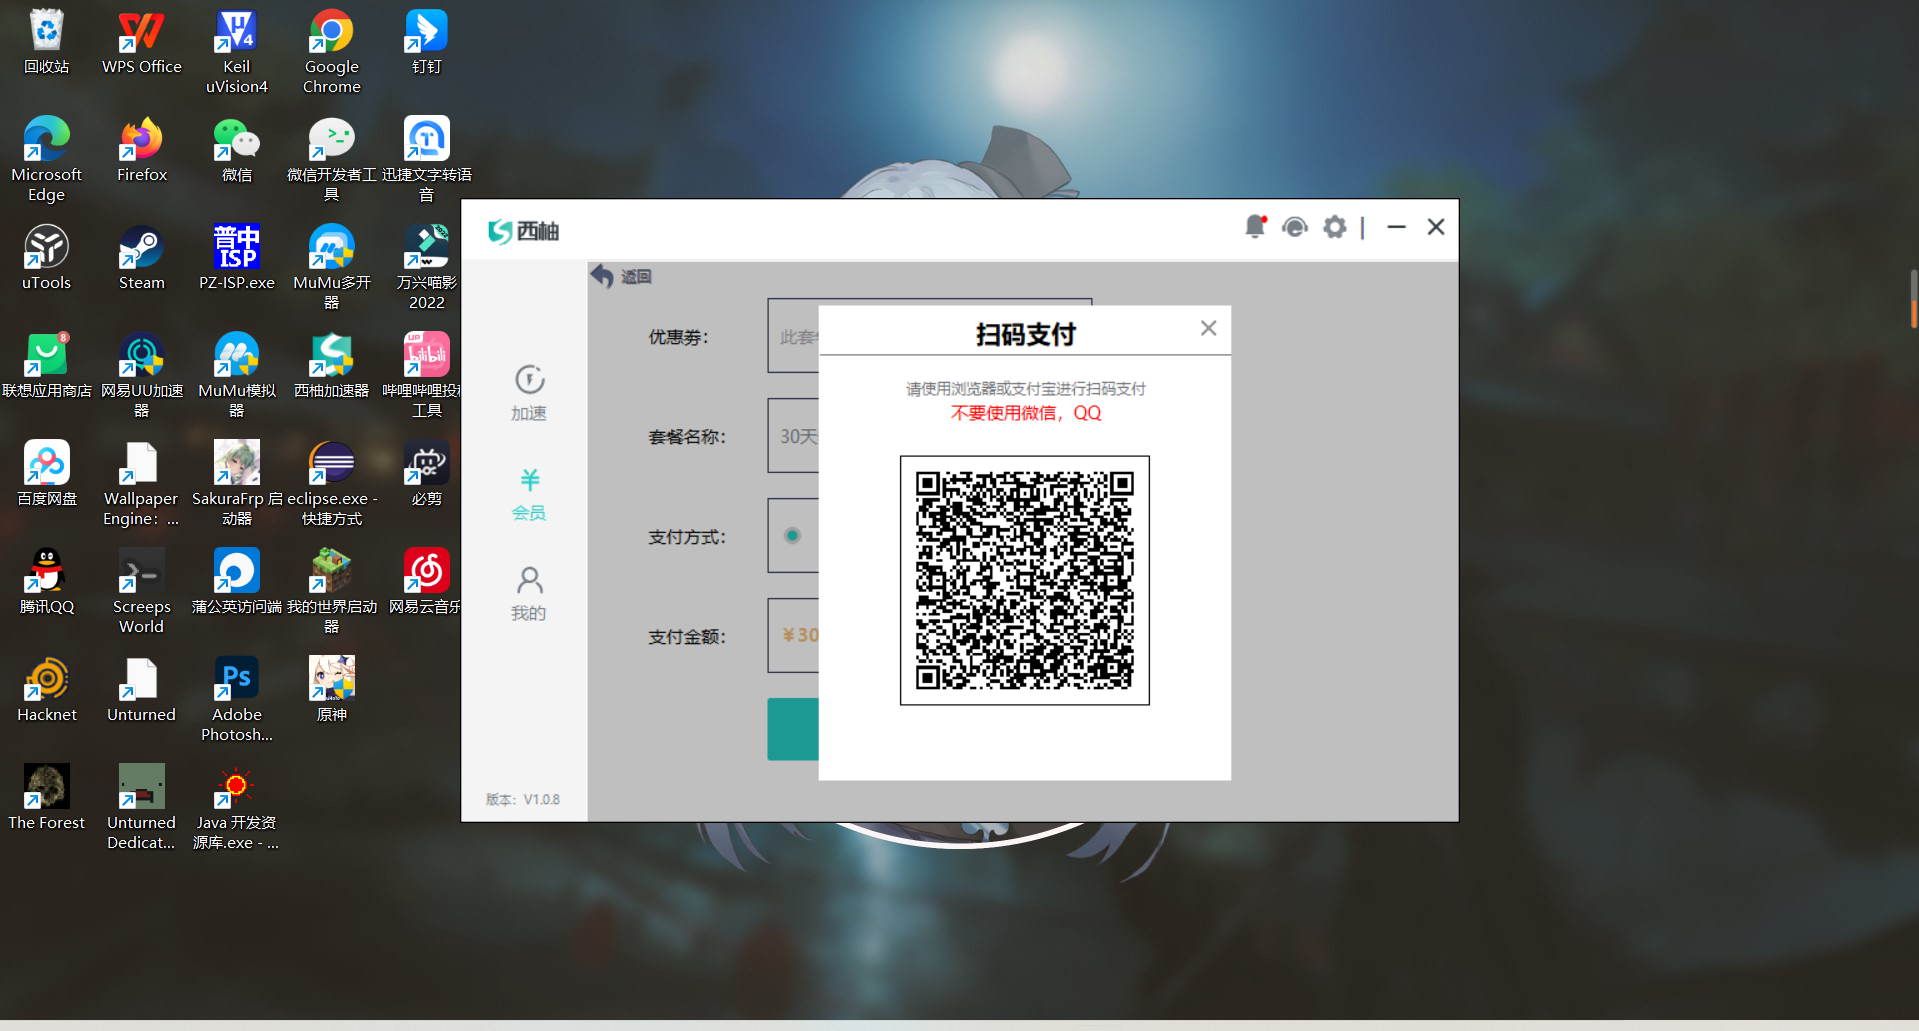
\includegraphics[width=0.6\linewidth]{1.png}
			\caption{VPN服务}
			\label{fig:dist}
		\end{figure}
	\subsection{申请Github账号}
		\begin{enumerate}
			\item{通过网址:https://github.com 进入Github主页,进入主页后可通过qq邮箱等注册一个Github账号,具体操作步骤请根据引导进行即可}(详情请看图3至图6)
		\end{enumerate}
\begin{figure}[htbp]
	\centering
	\subfigure{
		\begin{minipage}{4.5cm}
			\centering
			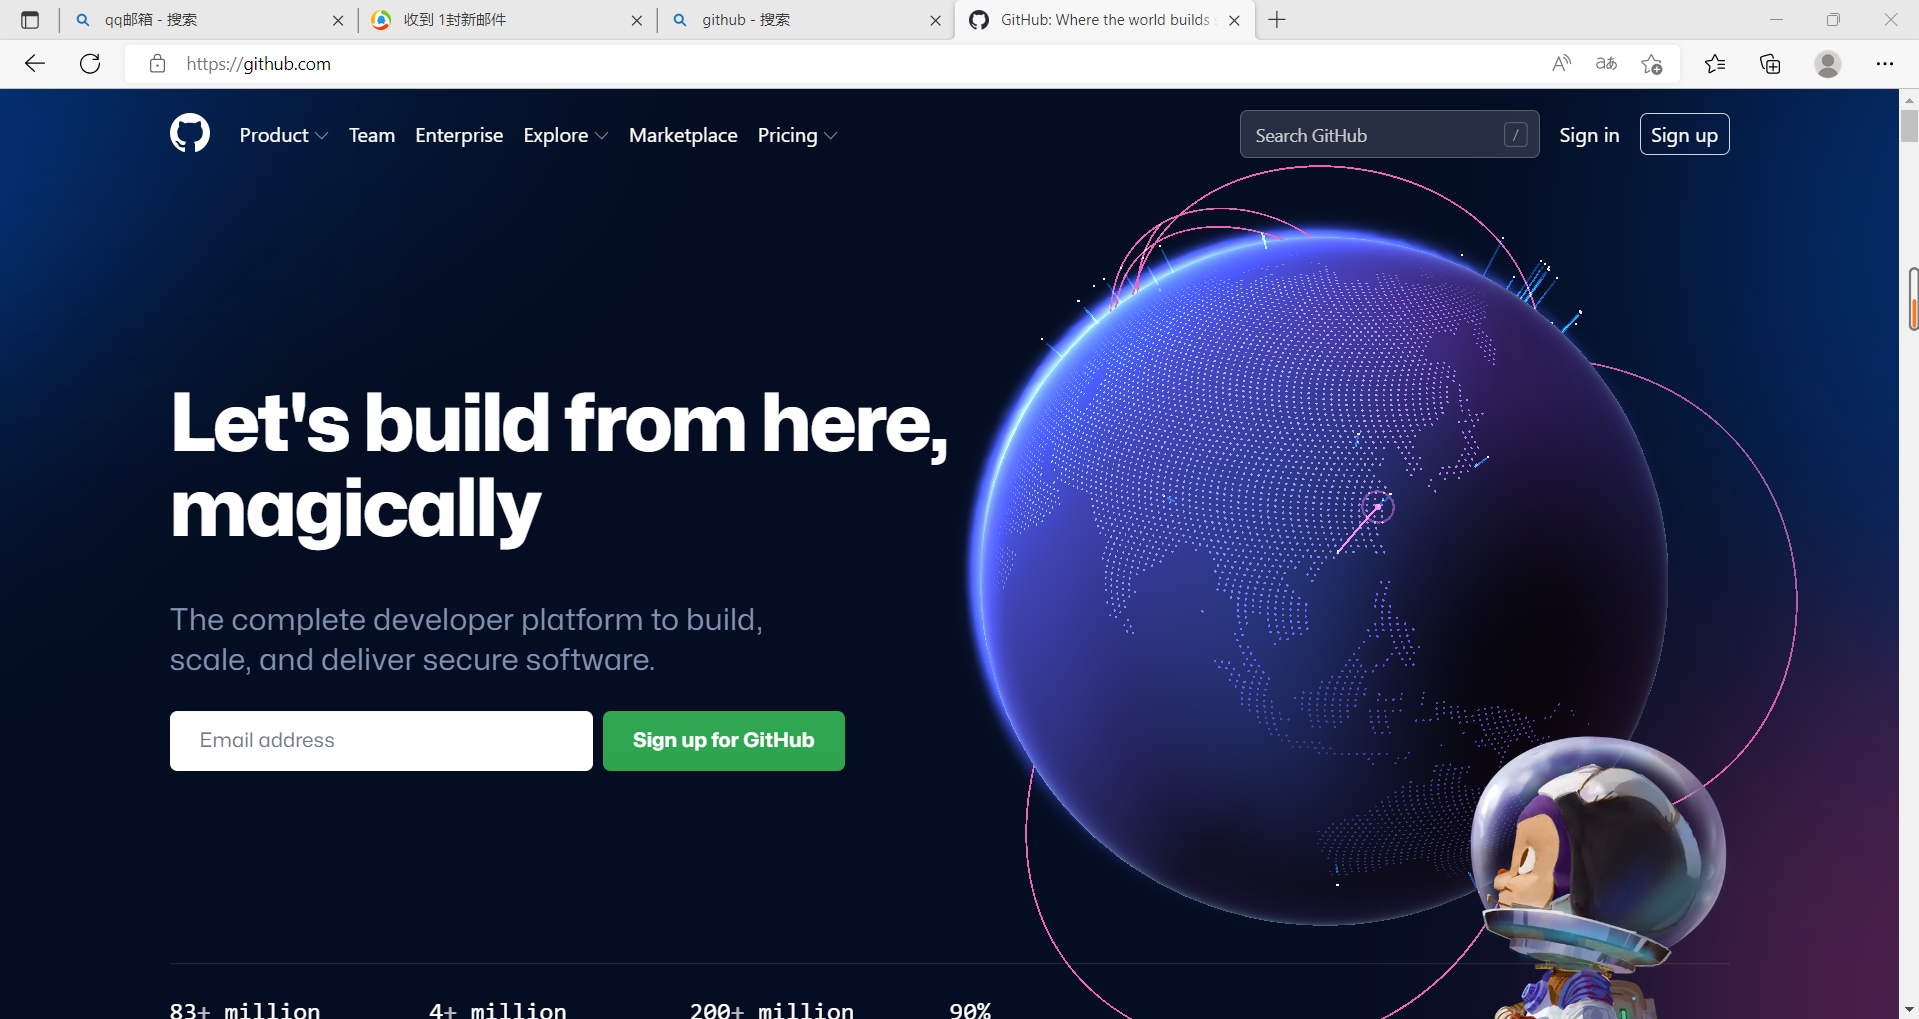
\includegraphics[width=5cm]{web1.png}
			\caption{主页}
		\end{minipage}%
	}%
	\subfigure{
		\begin{minipage}{7cm}
			\centering
			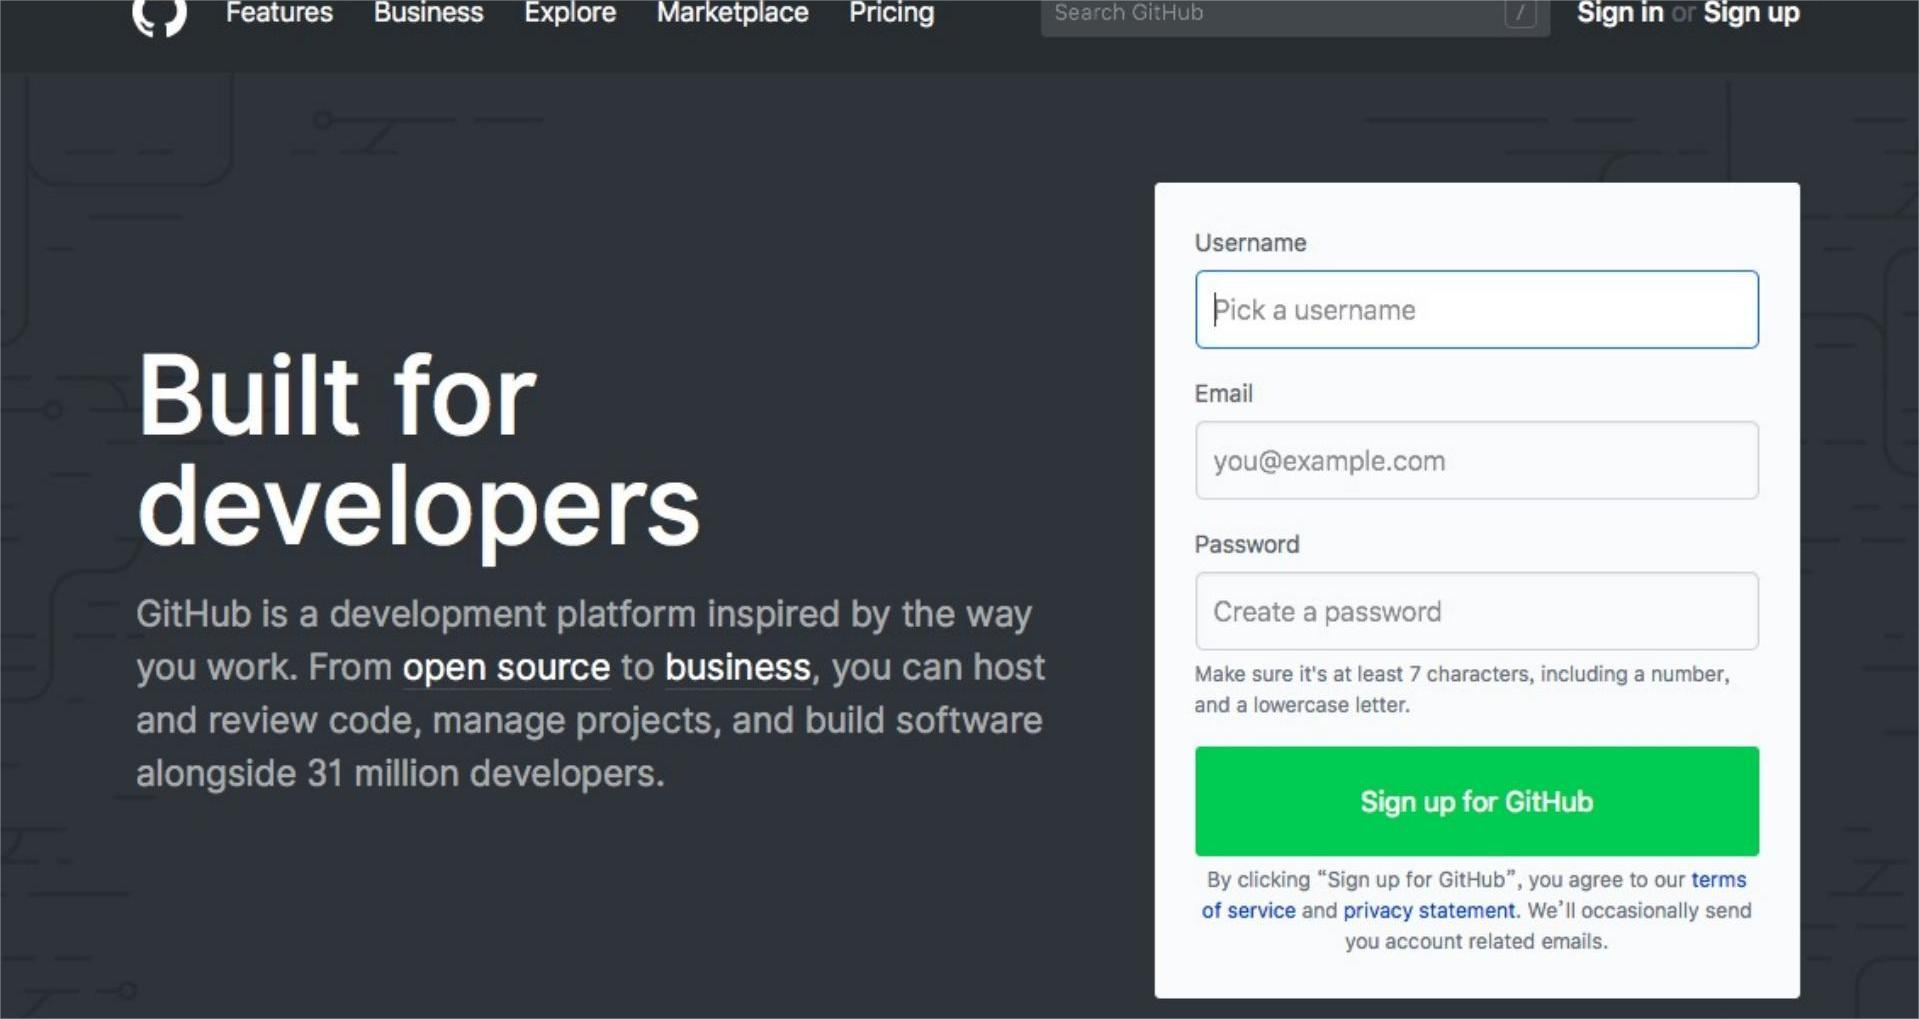
\includegraphics[width=5cm]{web2.png}
			\caption{注册页}
		\end{minipage}
	}
	\subfigure{
		\begin{minipage}{4.5cm}
			\centering
			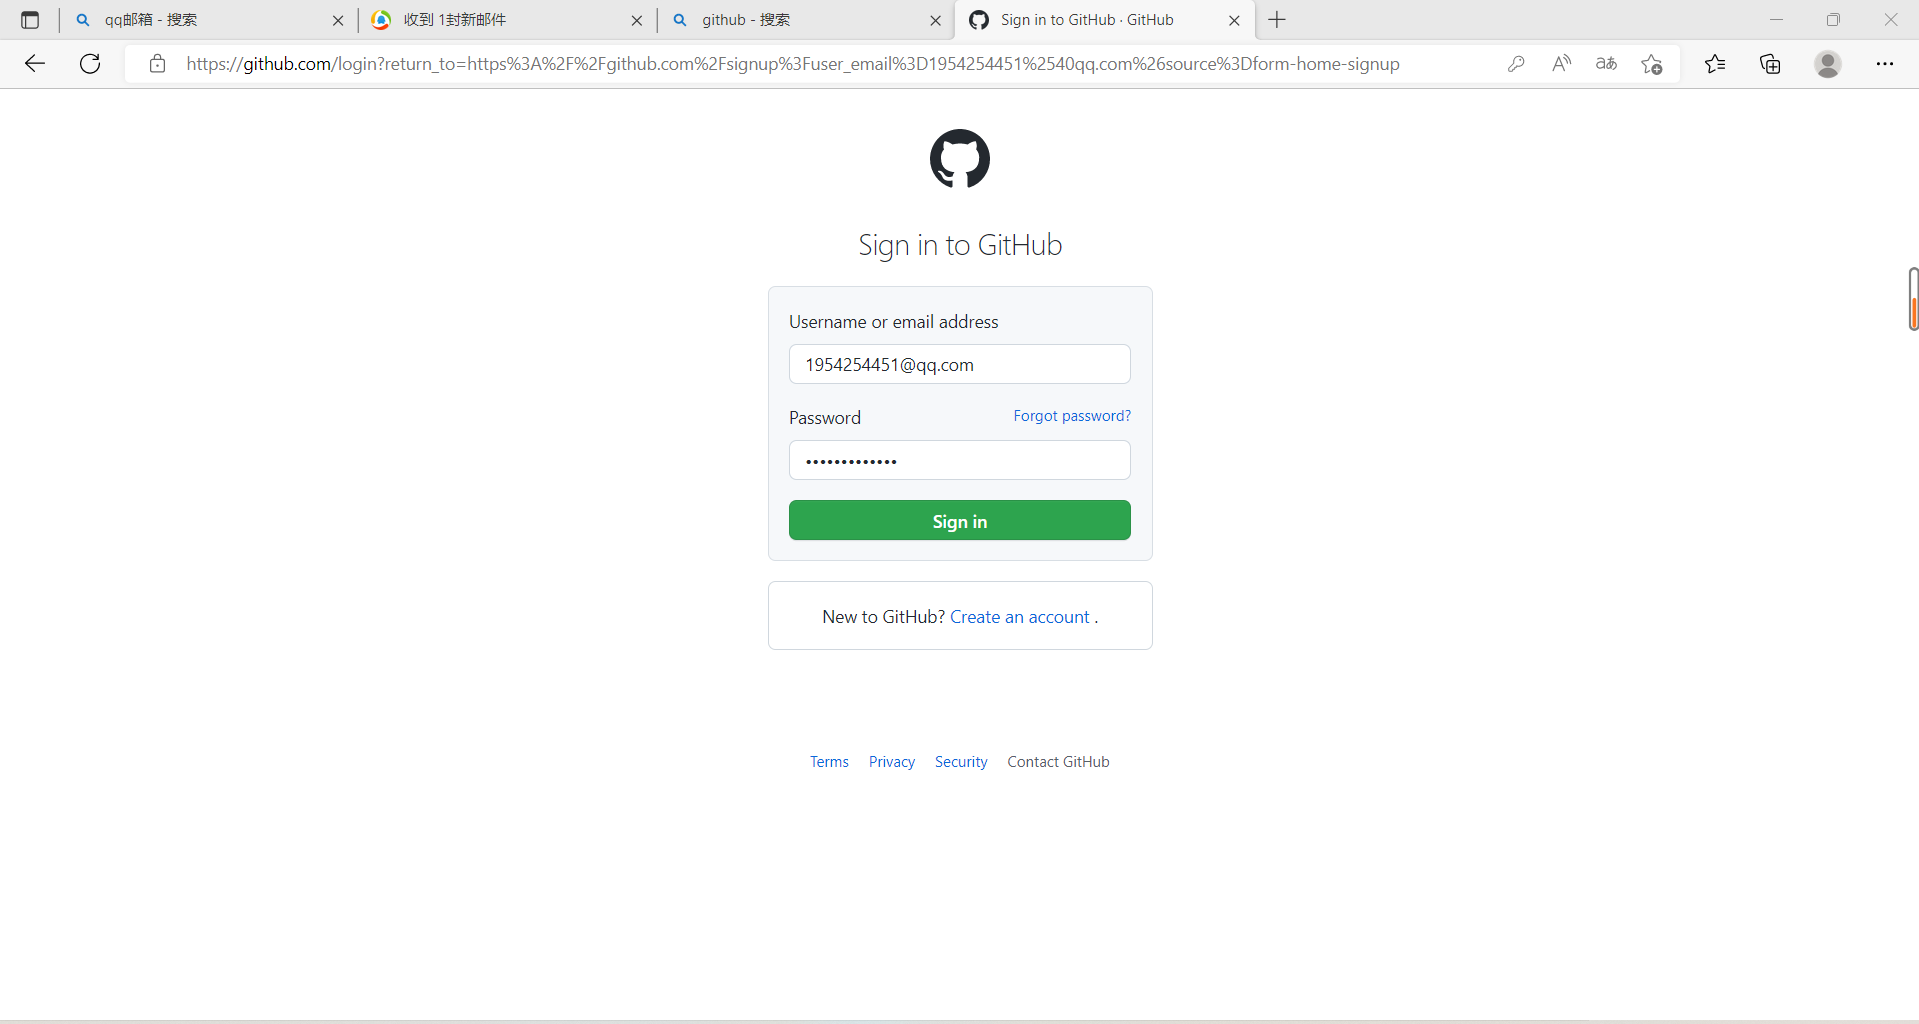
\includegraphics[width=5cm]{web3.png}
			\caption{登录页}
		\end{minipage}%
	}%
	\subfigure{
		\begin{minipage}{7cm}
			\centering
			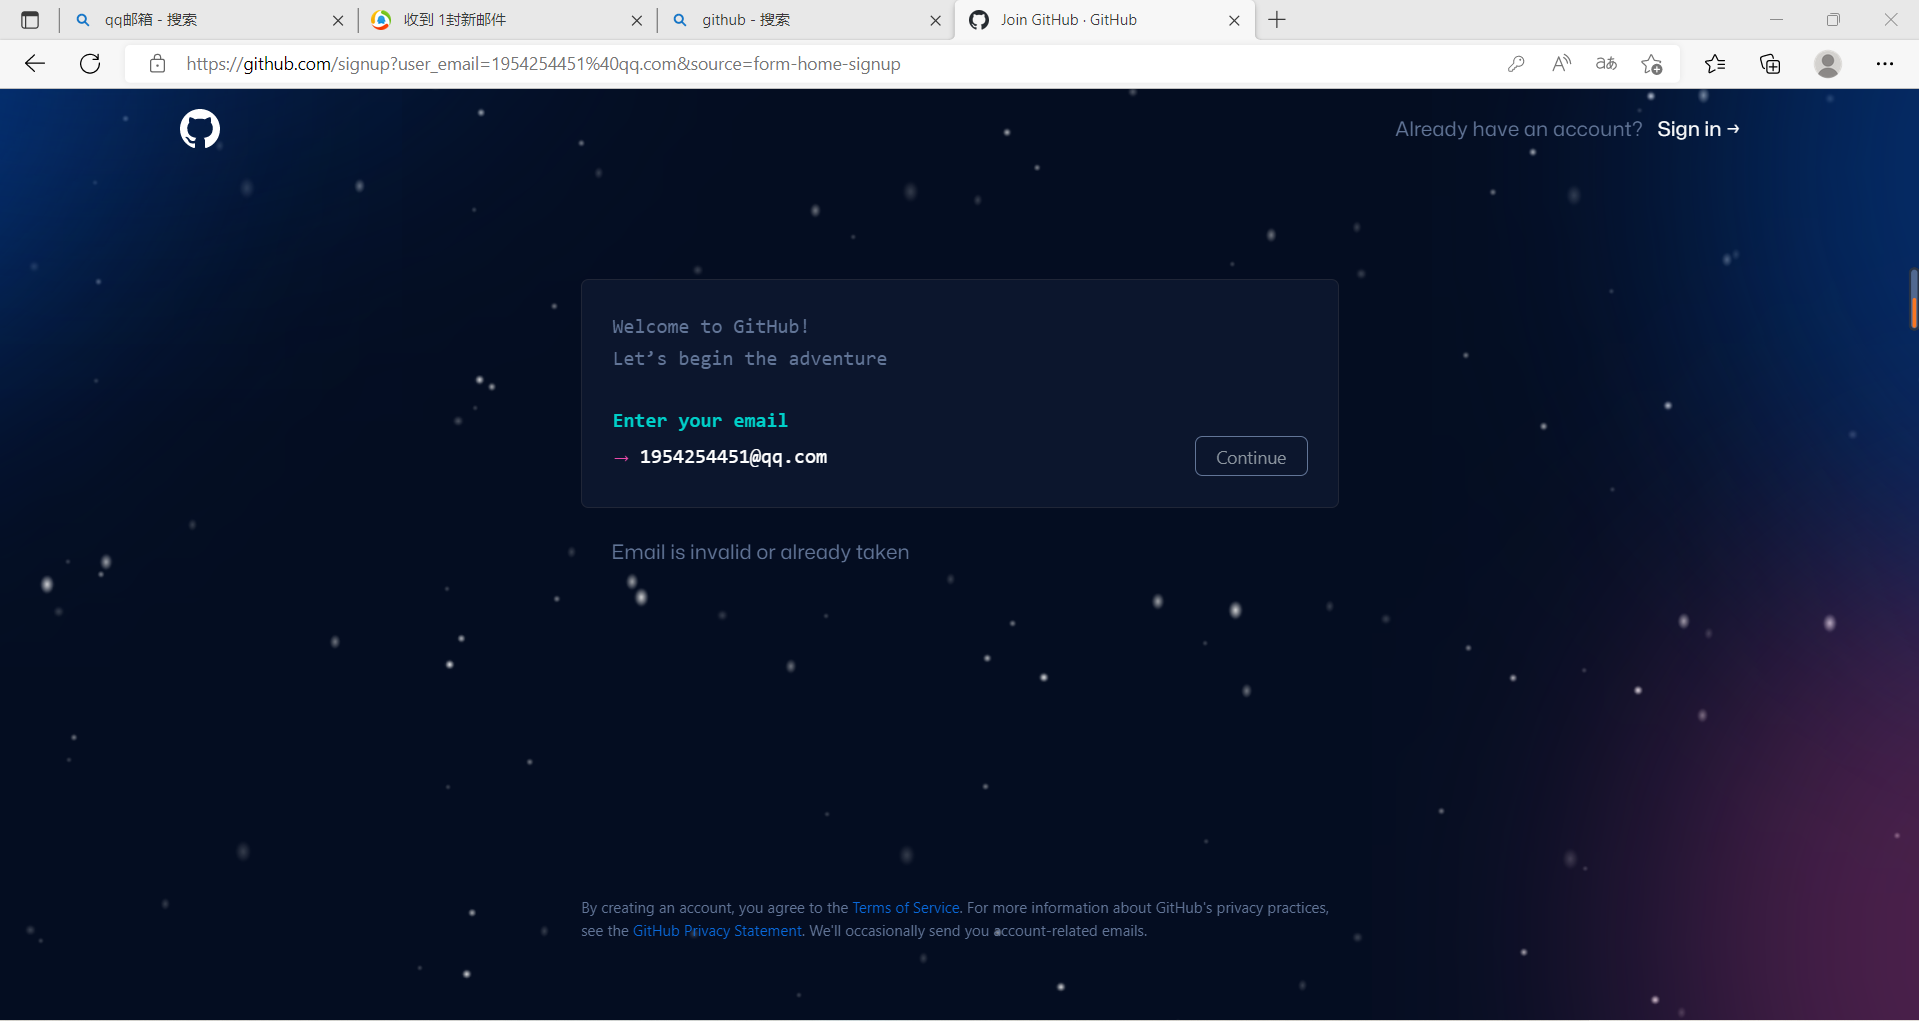
\includegraphics[width=5cm]{web4.png}
			\caption{登录页}
		\end{minipage}
	}
\end{figure}
	
	
	
	\subsection{安装并配置Git}
	\begin{enumerate}
		\item 由于sudo是linux的系统管理指令,而本人用的是windows操作系统,所以选择在官网下载安装(https://git-scm.com/download/win)
		\lstinputlisting[language=MATLAB]{code/command1.m}
		\item{打开Git Bash命令行输入对应配置命令,配置用户信息,如下图所示:}
		\lstinputlisting[language=MATLAB]{code/command2.m}
		\begin{figure}[!htbp]
			\centering
			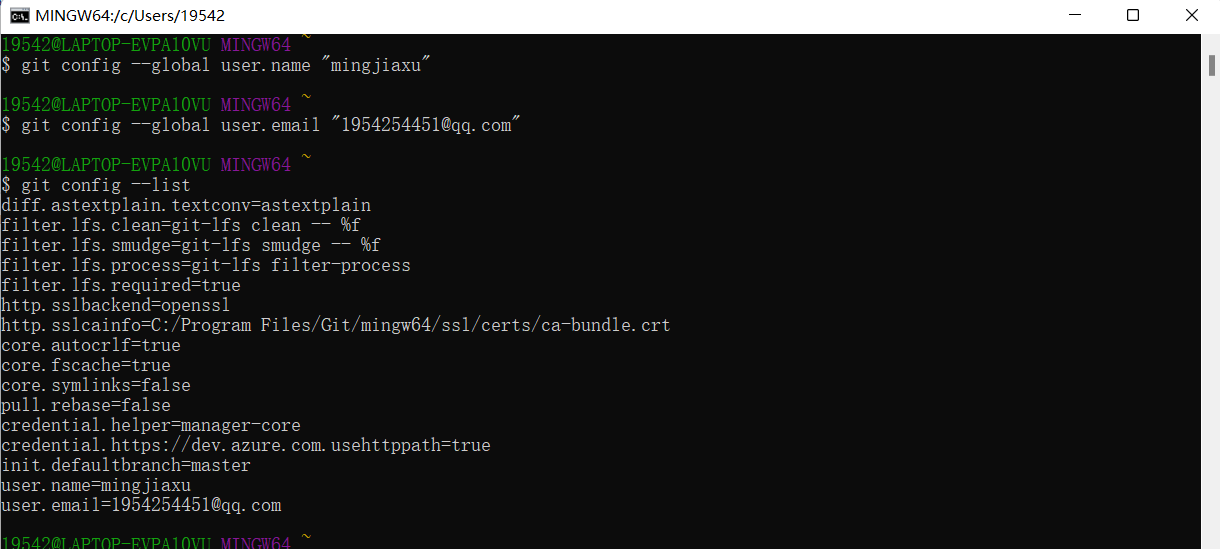
\includegraphics[width=0.6\linewidth]{pezhi.png}
			\caption{配置用户信息}
			\label{fig:dist}
		\end{figure}
	\end{enumerate}
	\subsection{安装ssh并于Github添加公钥}
		\begin{enumerate}
			\item{下载安装ssh}与安装Git时情况相同,我们无法直接使用sudo命令直接下载ssh,同样的,我选择了在官网下载,我选择的是OpenSSH-Win64.zip(https://github.com/PowerShell/Win32-OpenSSH/releases ),如下图所示
			\lstinputlisting[language=MATLAB]{code/command3.m}
			\begin{figure}[!htbp]
				\centering
				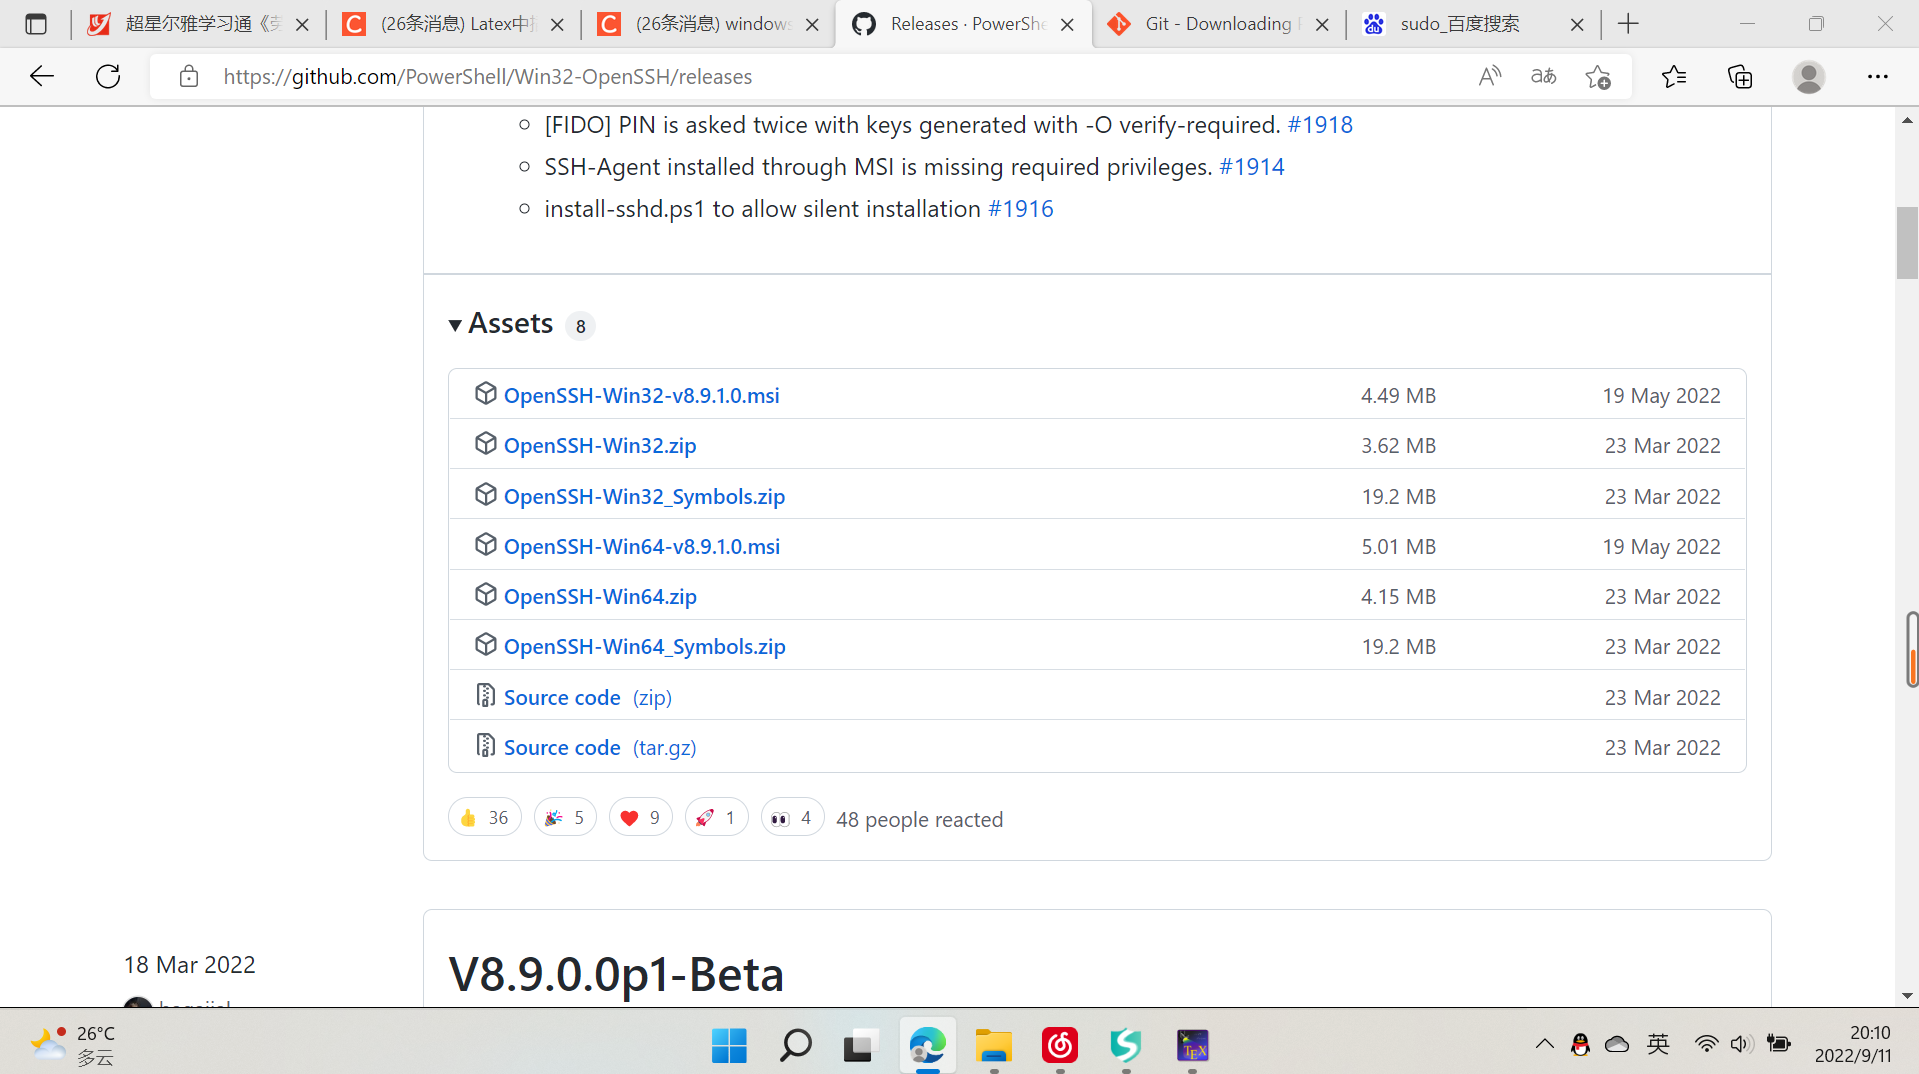
\includegraphics[width=0.6\linewidth]{ssh.png}
				\caption{ssh下载页面}
				\label{fig:dist}
			\end{figure}
			\item{创建密钥文件}win+r打开cmd,输入以下指令,啥都不用填,直接回车过。
			\lstinputlisting[language=MATLAB]{code/command4.m}
		
			\item{将公钥添加到Github}
				\subitem{查看生成公钥} 
					找到.ssh文件夹(文件路径基本都一样,只是名字不同)
					在如图所示位置输入cmd打开命令行,输入以下指令查看公钥,直接打开$id_rsa$文件可能打不开
					
					\lstinputlisting[language=MATLAB]{code/command5.m}
					
					\begin{figure}[htbp]
					\centering
					\subfigure{
						\begin{minipage}{4.5cm}
							\centering
							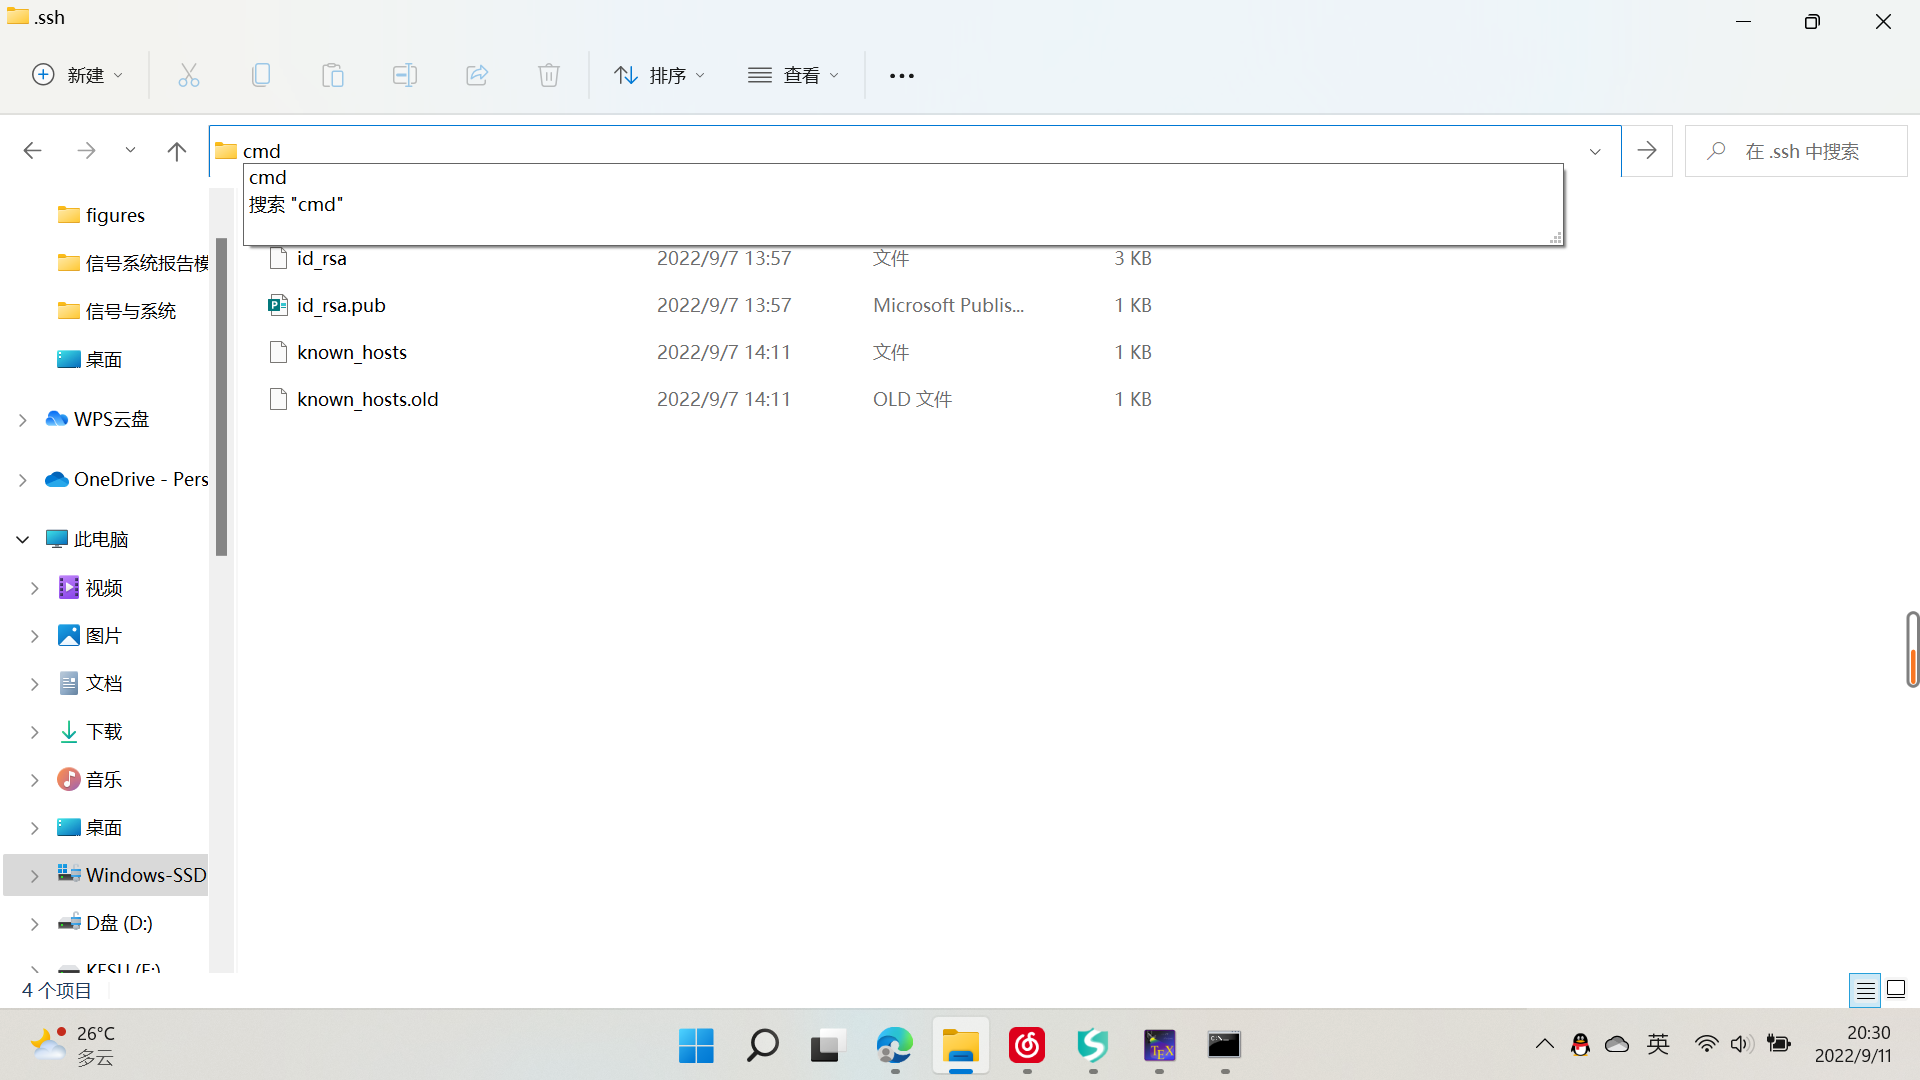
\includegraphics[width=5cm]{cmd2.png}
							\caption{命令行打开位置}
						\end{minipage}
					}
					\subfigure{
						\begin{minipage}{7cm}
							\centering
							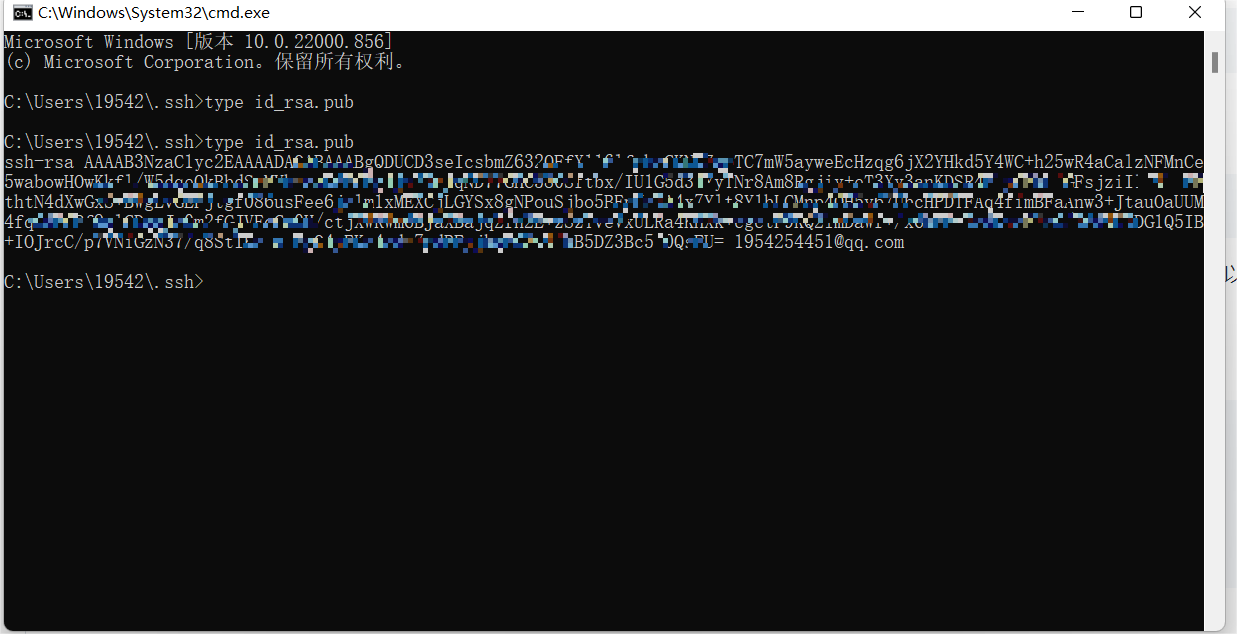
\includegraphics[width=5cm]{cmd3.png}
							\caption{命令行指令输入}
						\end{minipage}
					}
				\end{figure}
				\subitem{添加公钥至Github:} 
					在头像处找到 Setting 双击打开,然后找到SSH and GPG keys 选项 ,点击后找到new ssh key 打开后粘贴公钥 
				\begin{figure}[htbp]
					\centering
					\subfigure{
						\begin{minipage}{4.5cm}
							\centering
							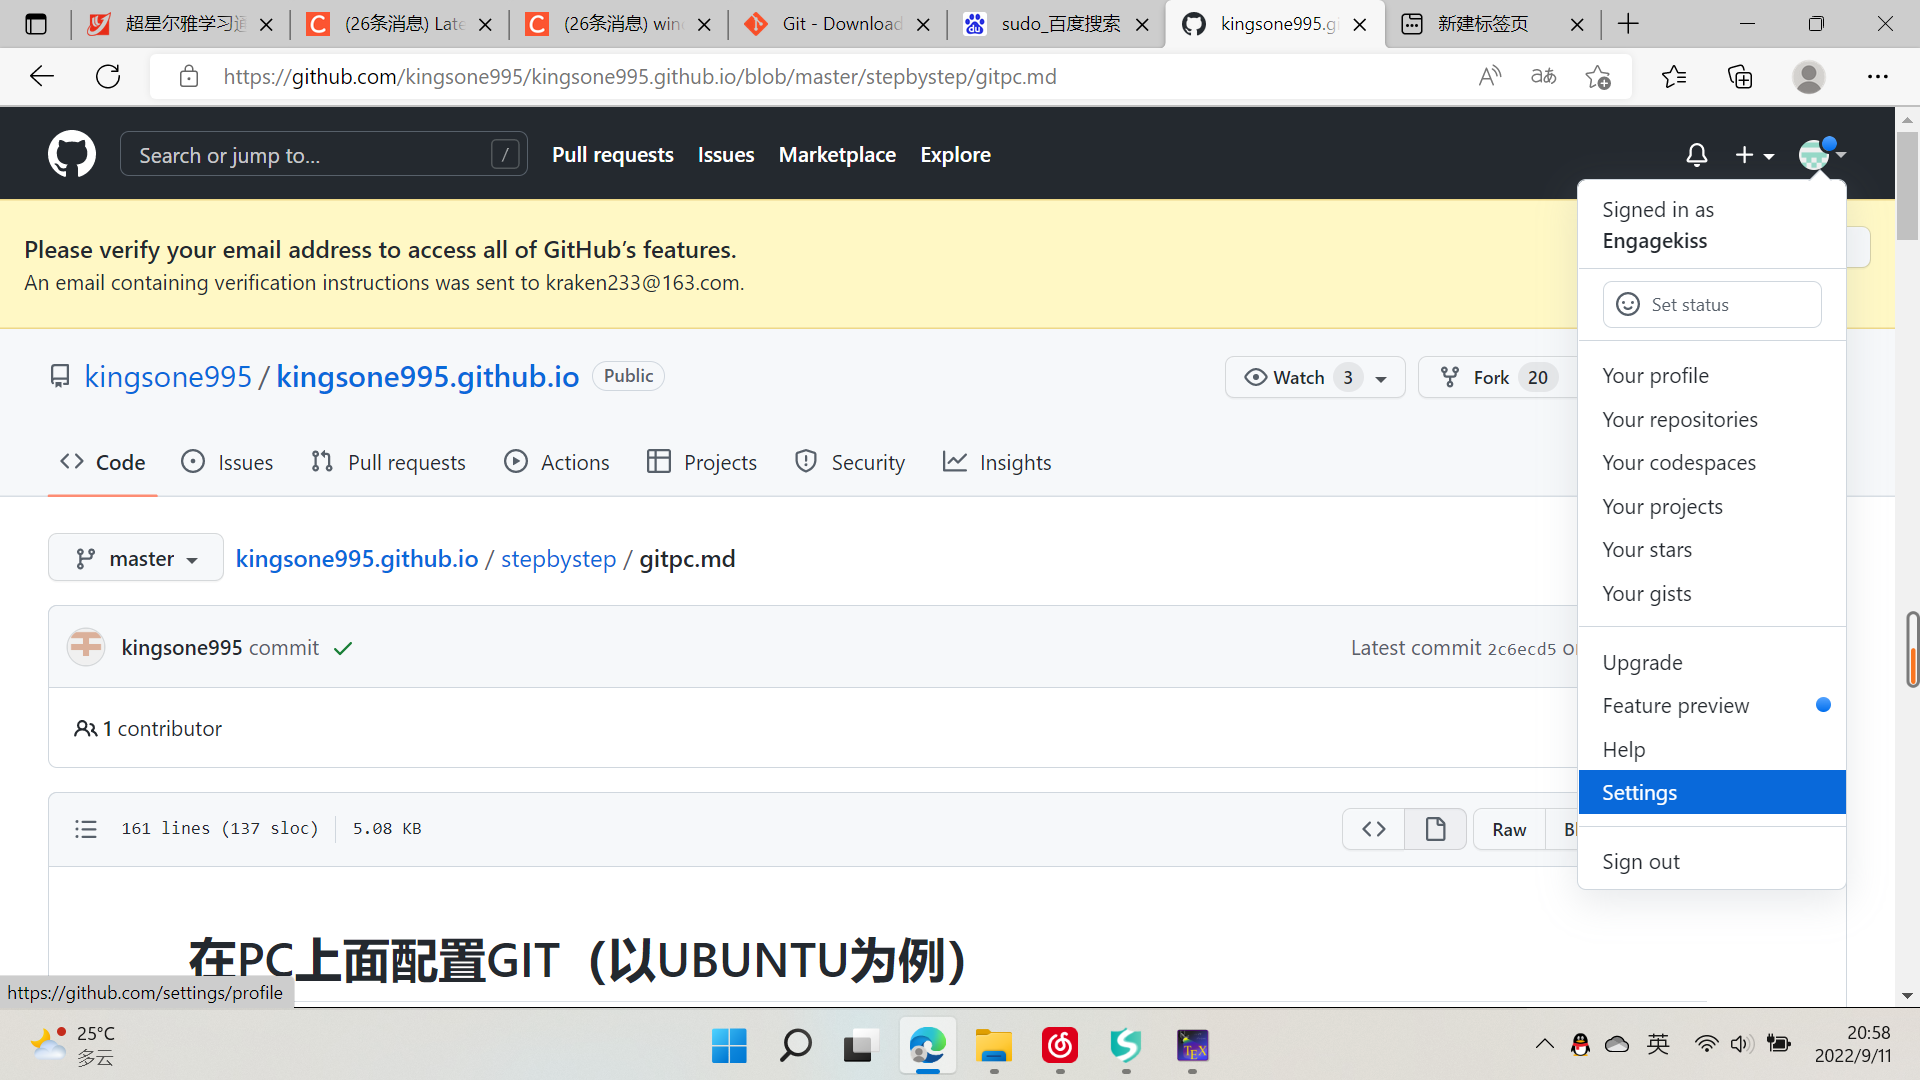
\includegraphics[width=5cm]{tianjia (1).png}
						\end{minipage}%
					}%
					\subfigure{
						\begin{minipage}{7cm}
							\centering
							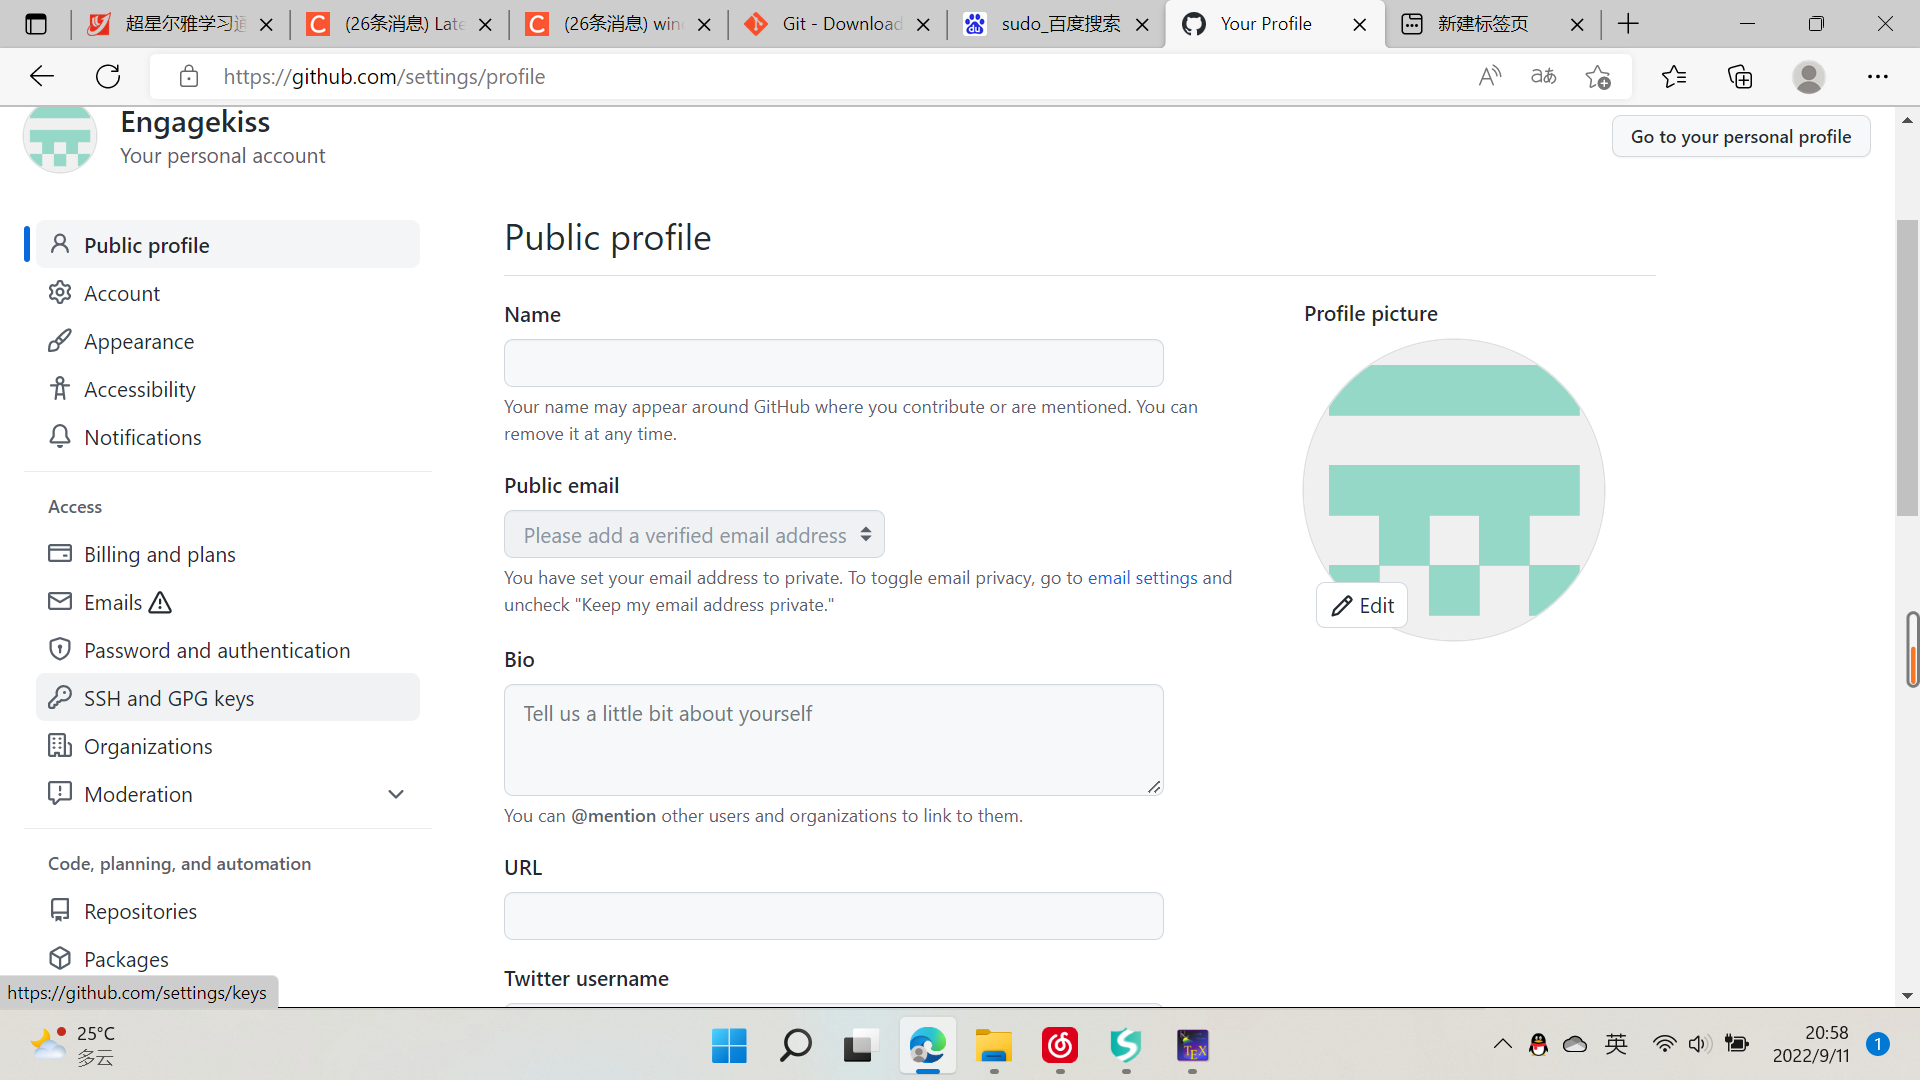
\includegraphics[width=5cm]{tianjia (2).png}
						\end{minipage}
					}
					\subfigure{
						\begin{minipage}{4.5cm}
							\centering
							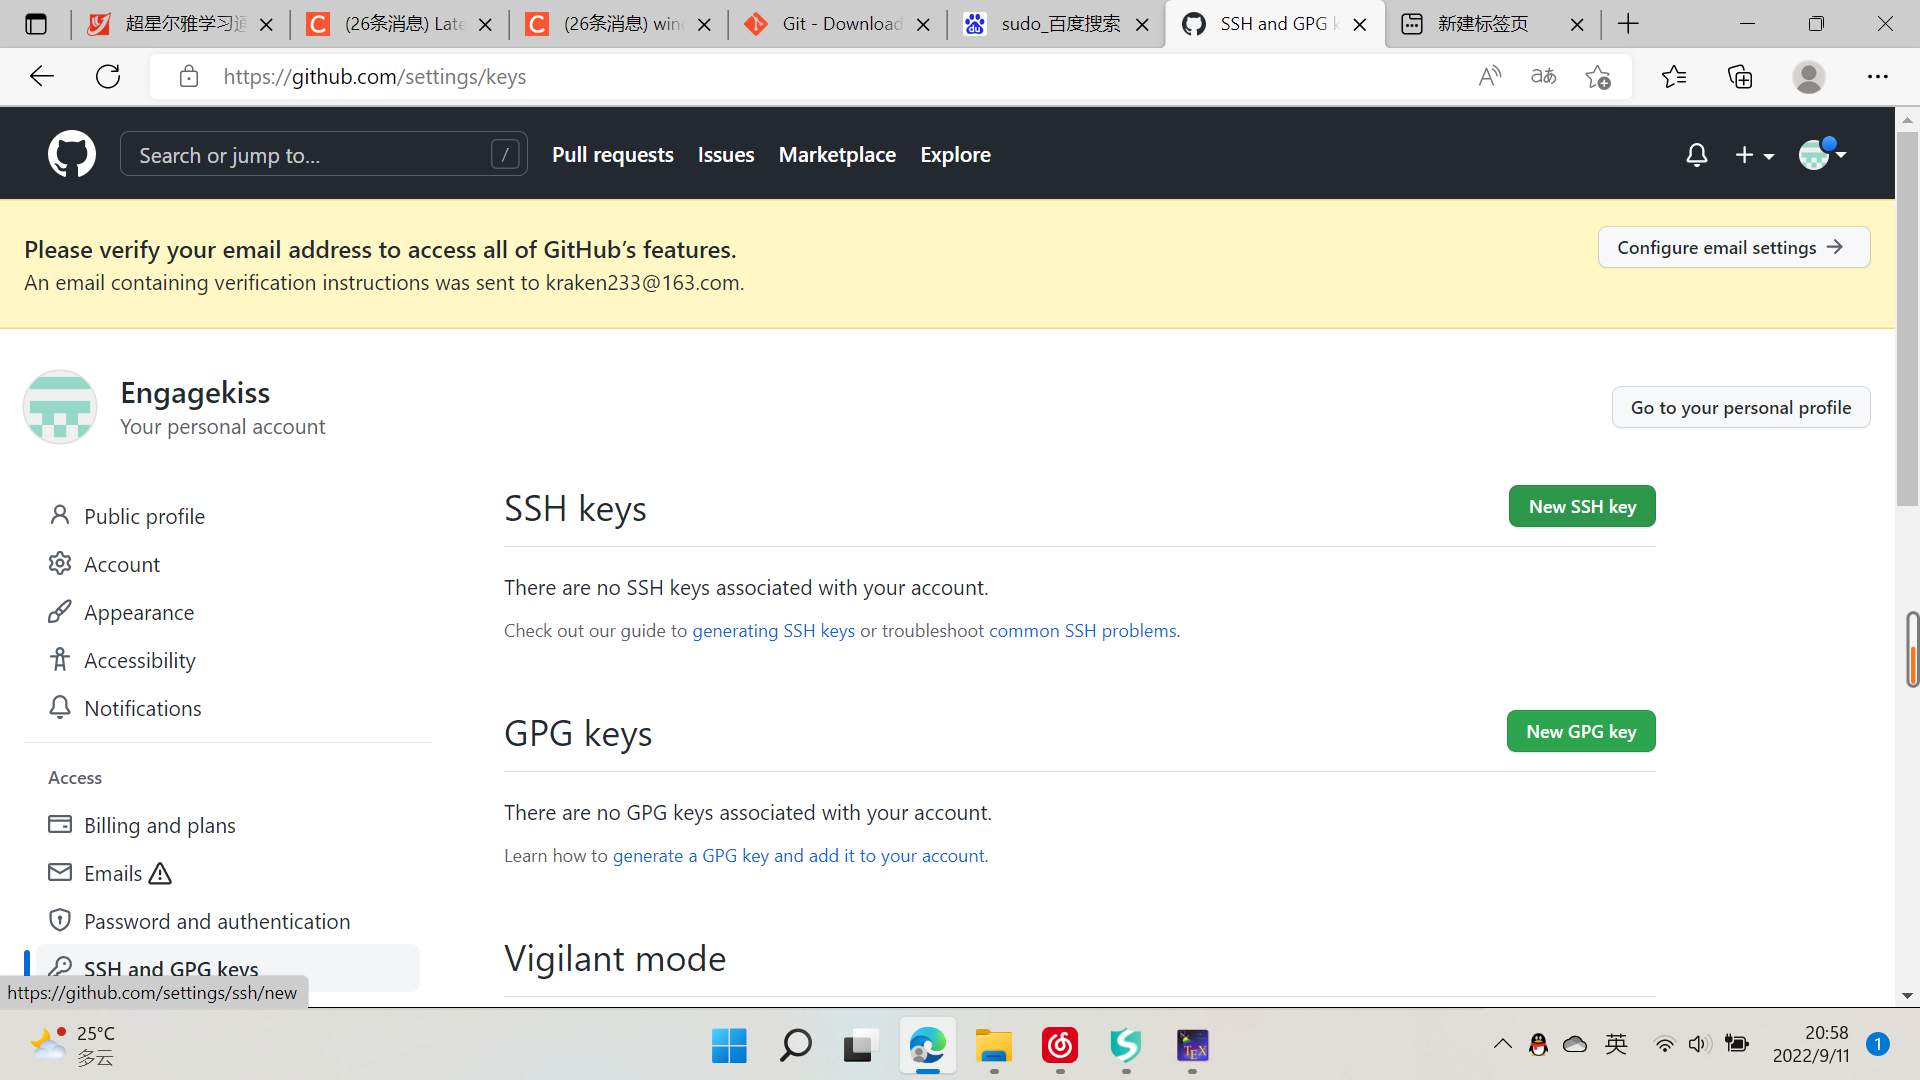
\includegraphics[width=5cm]{tianjia (3).png}
						\end{minipage}%
					}%
					\subfigure{
						\begin{minipage}{7cm}
							\centering
							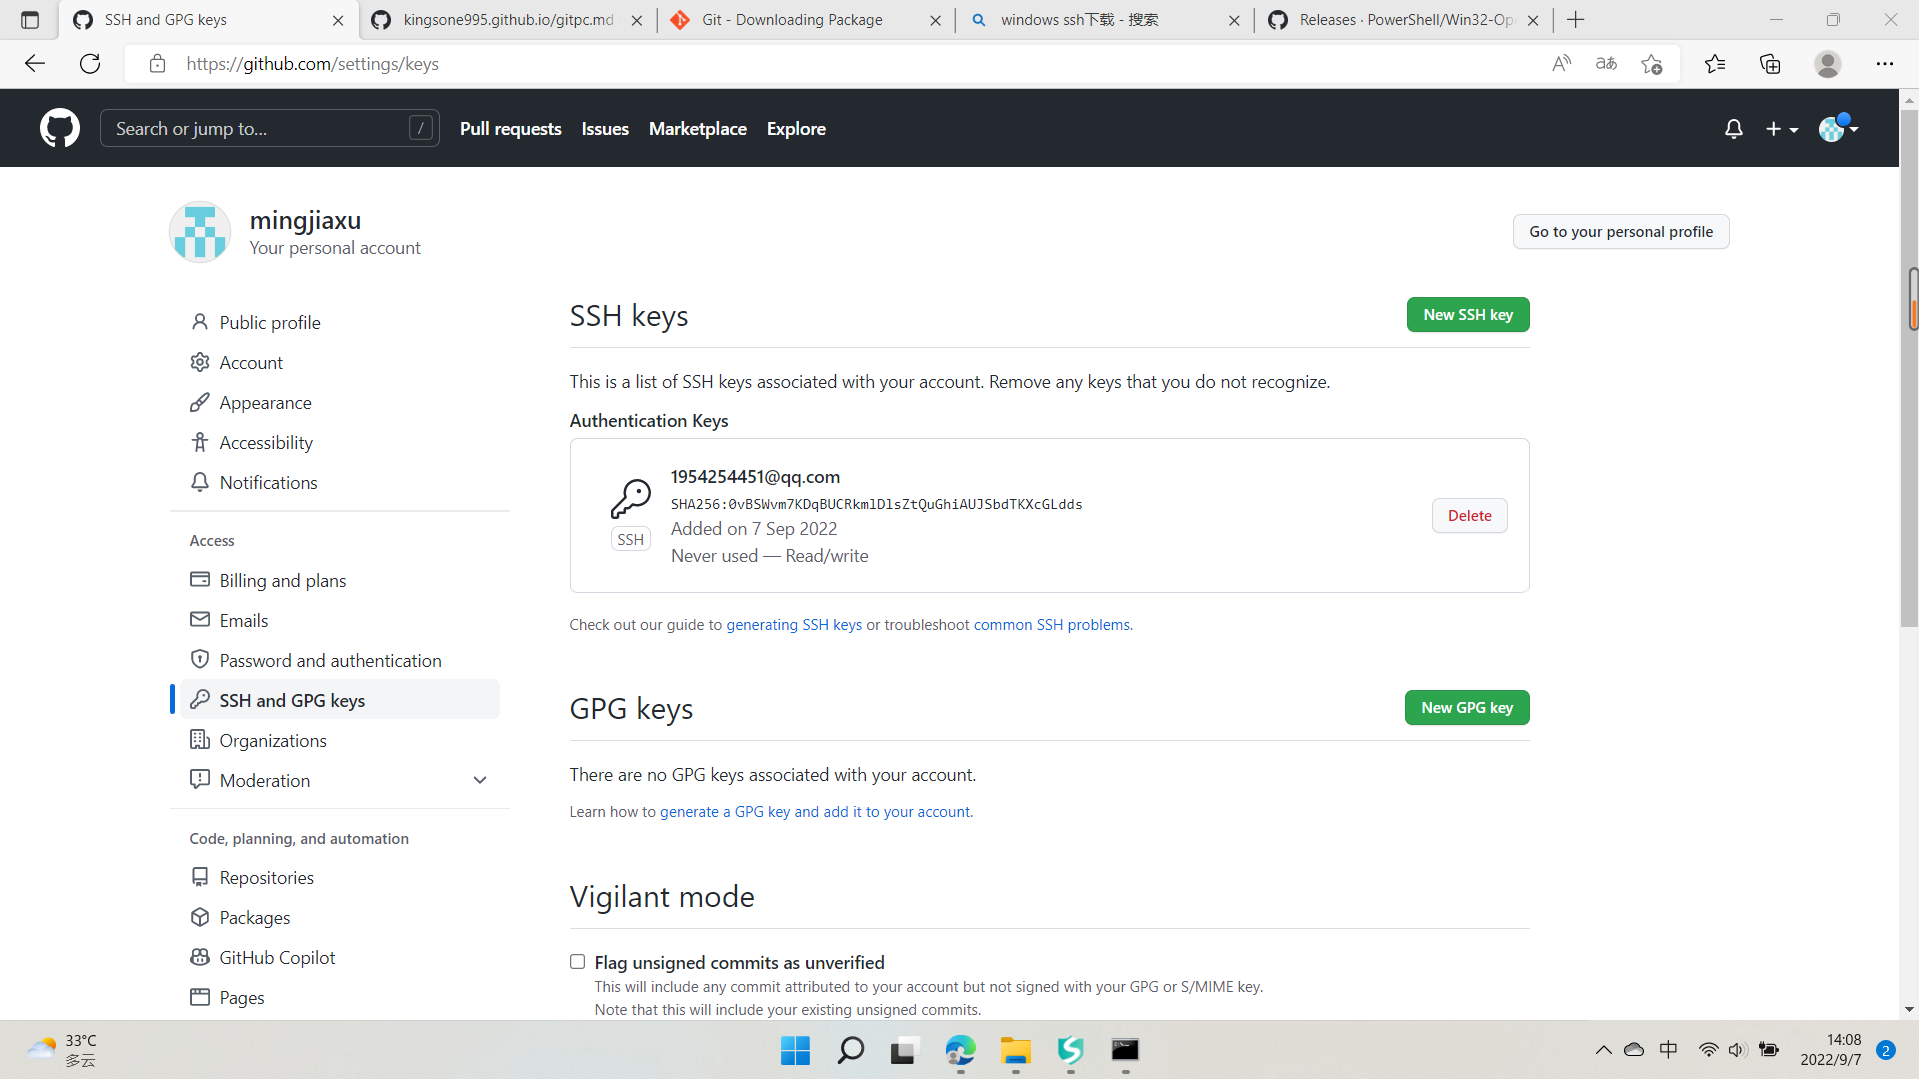
\includegraphics[width=5cm]{tianjia (4).png}
						\end{minipage}
					}
				\end{figure}
		\end{enumerate}
	
\section{实验内容}
	创建博客仓库并进行功能测试
	\subsection{在Github建立名为test的public仓库:具体操作如下图所示}
		\begin{figure}[htbp]
			\centering
			\subfigure{
				\begin{minipage}{4.5cm}
					\centering
					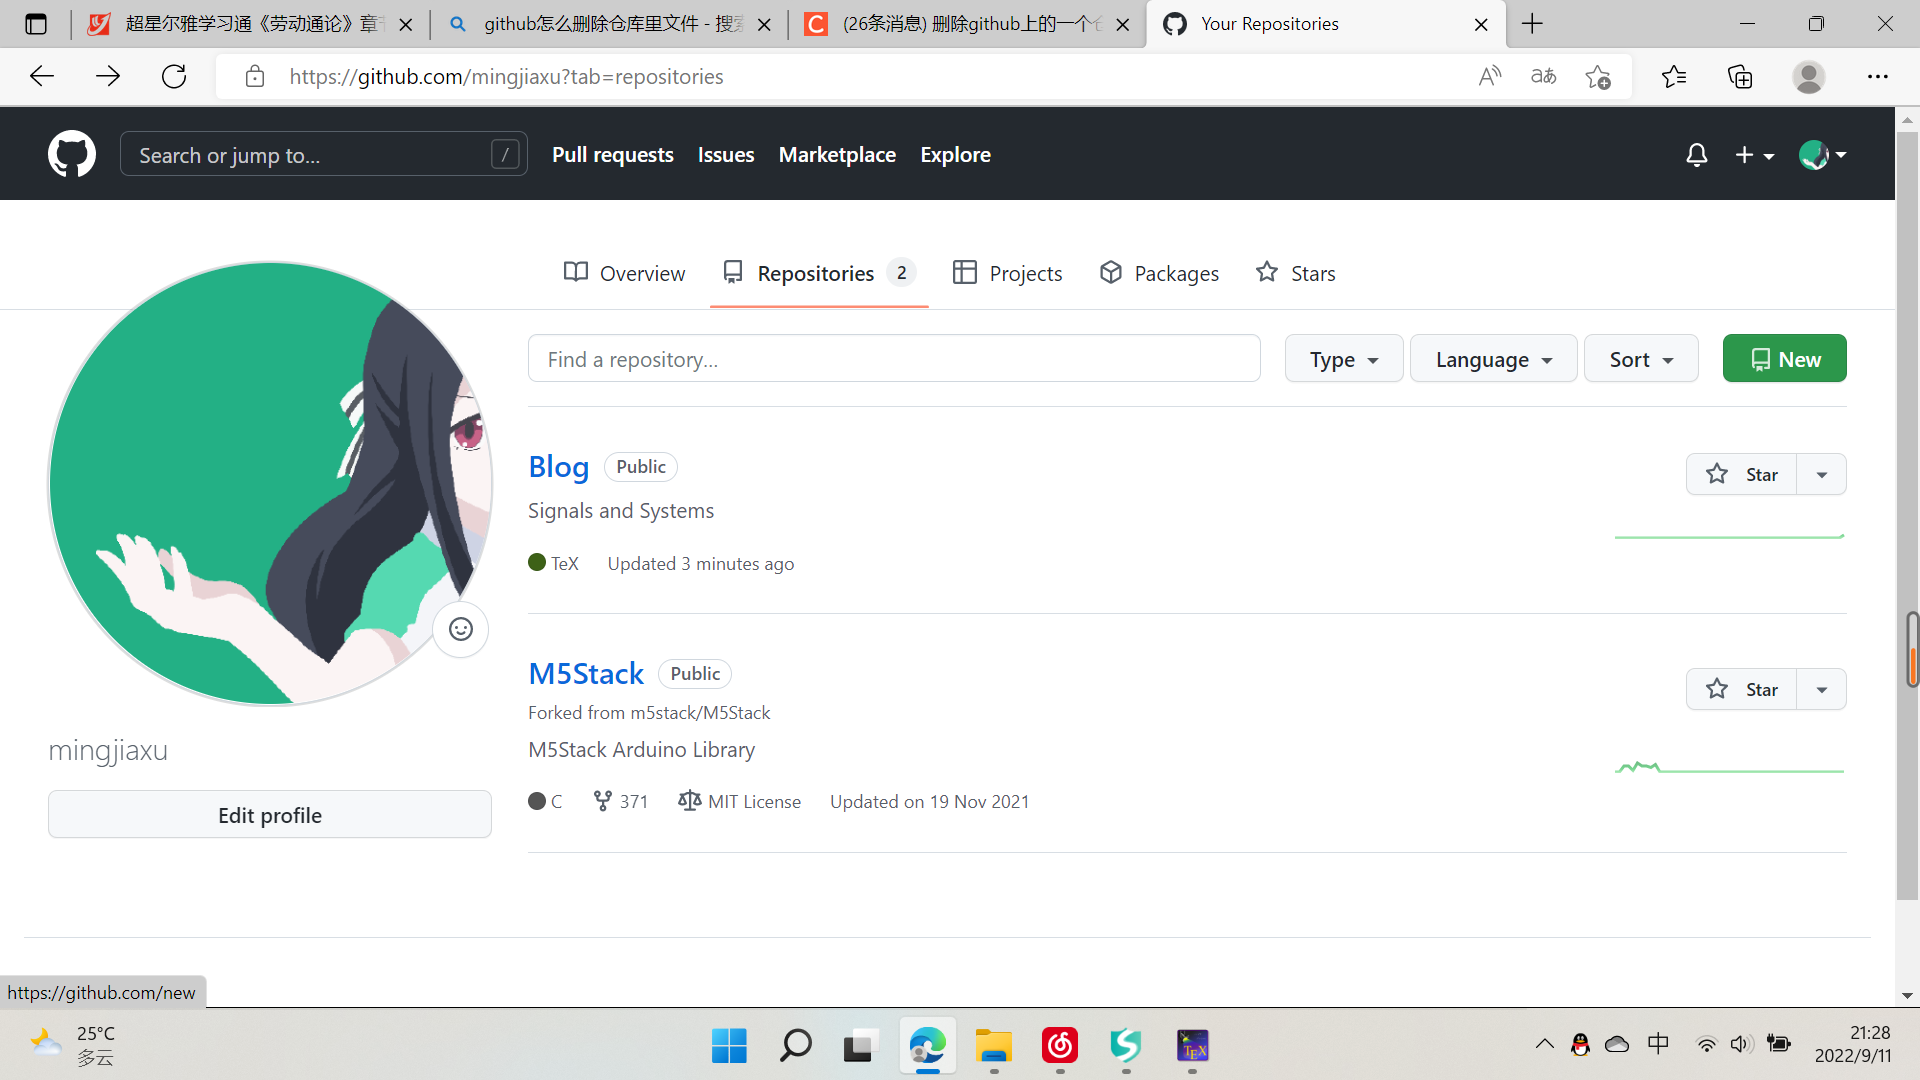
\includegraphics[width=5cm]{(1).png}
				\end{minipage}%
			}%
			\subfigure{
				\begin{minipage}{7cm}
					\centering
					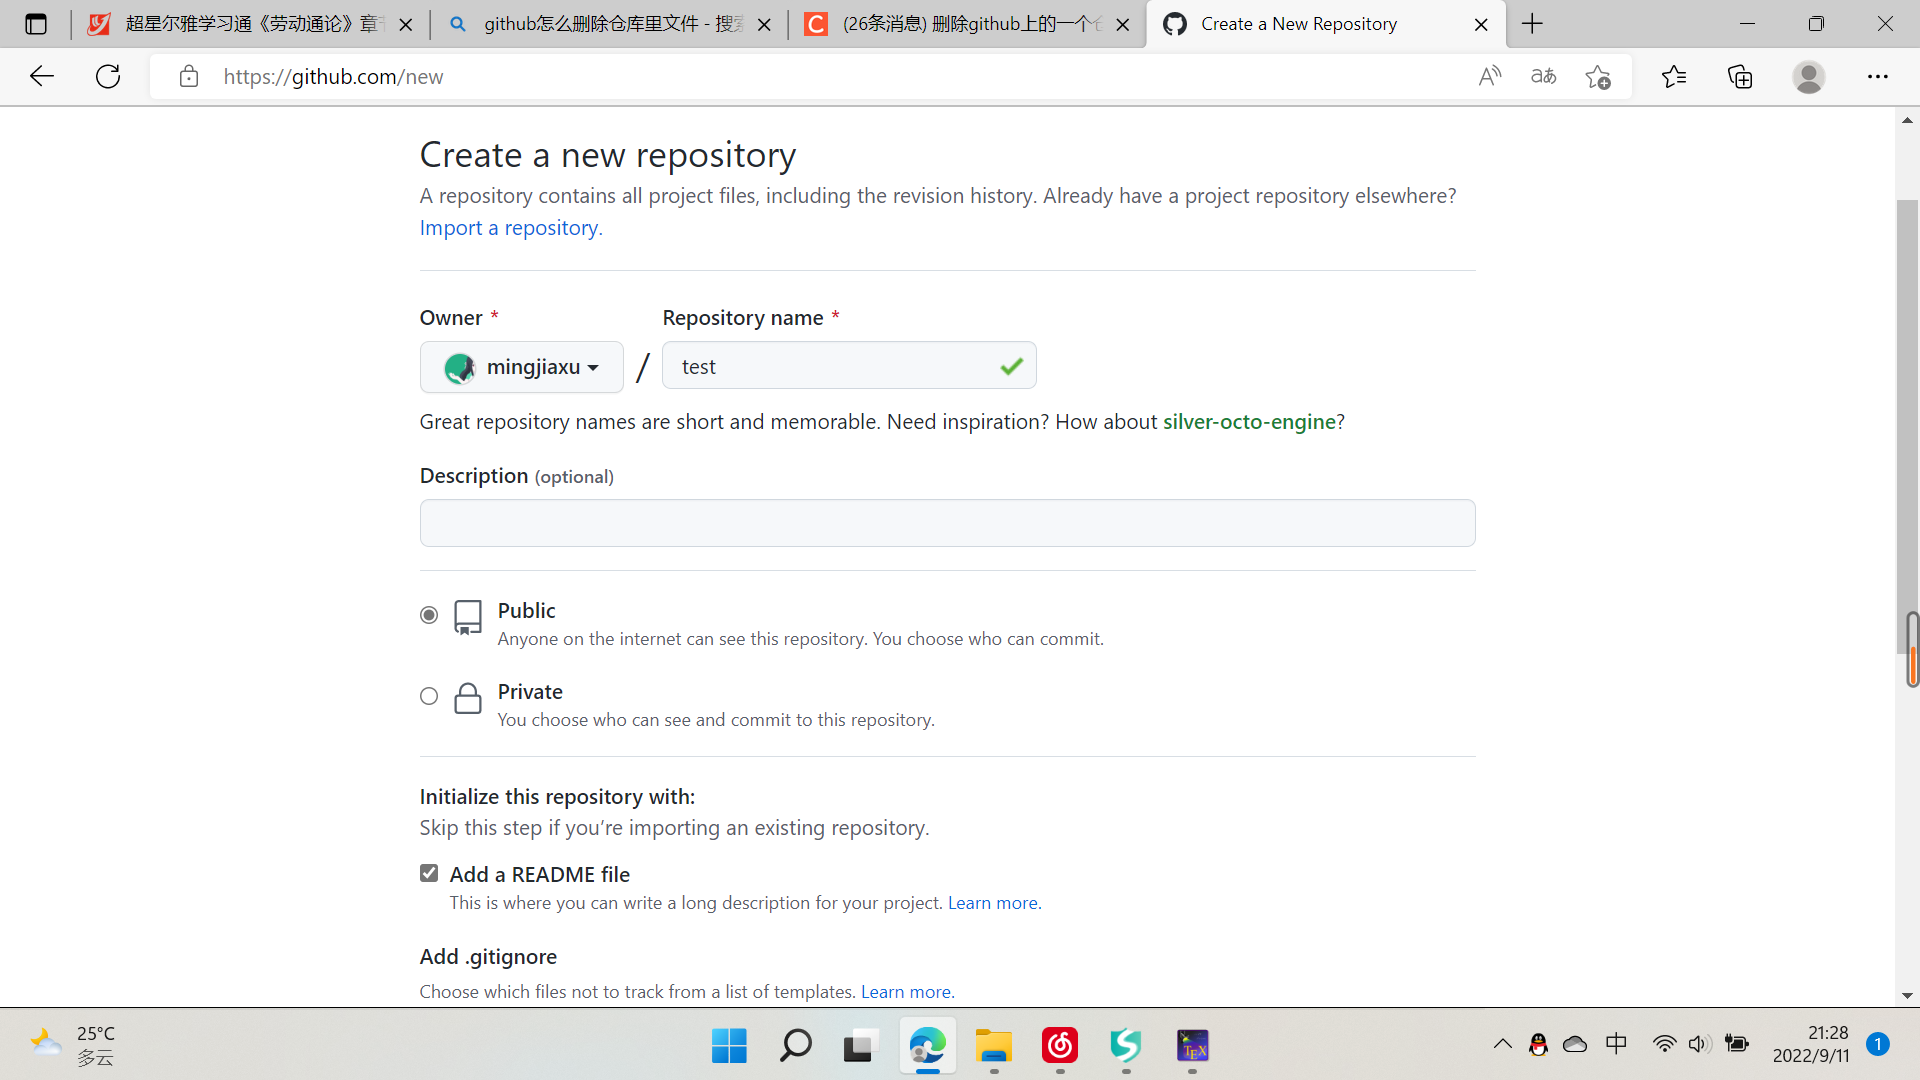
\includegraphics[width=5cm]{(2).png}
				\end{minipage}
			}
			\subfigure{
				\begin{minipage}{4.5cm}
					\centering
					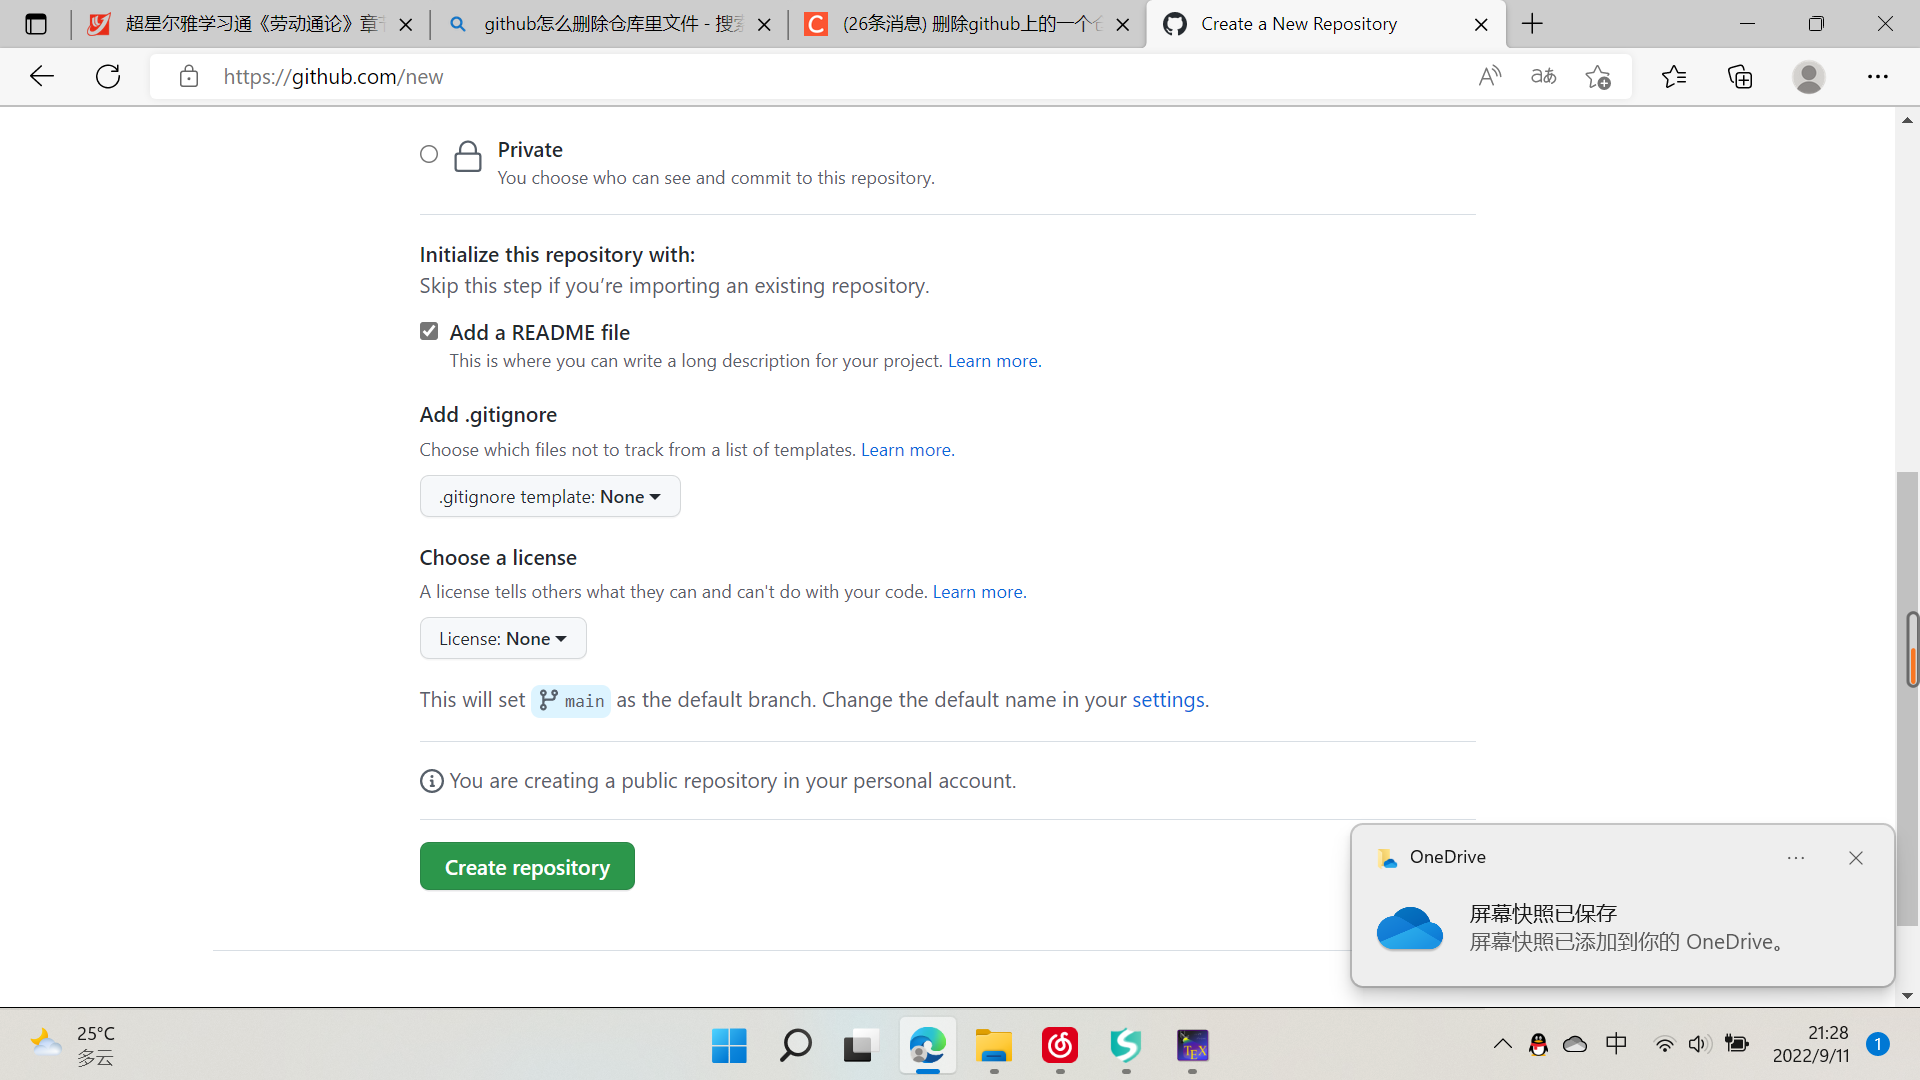
\includegraphics[width=5cm]{(3).png}
				\end{minipage}%
			}%
			\subfigure{
				\begin{minipage}{7cm}
					\centering
					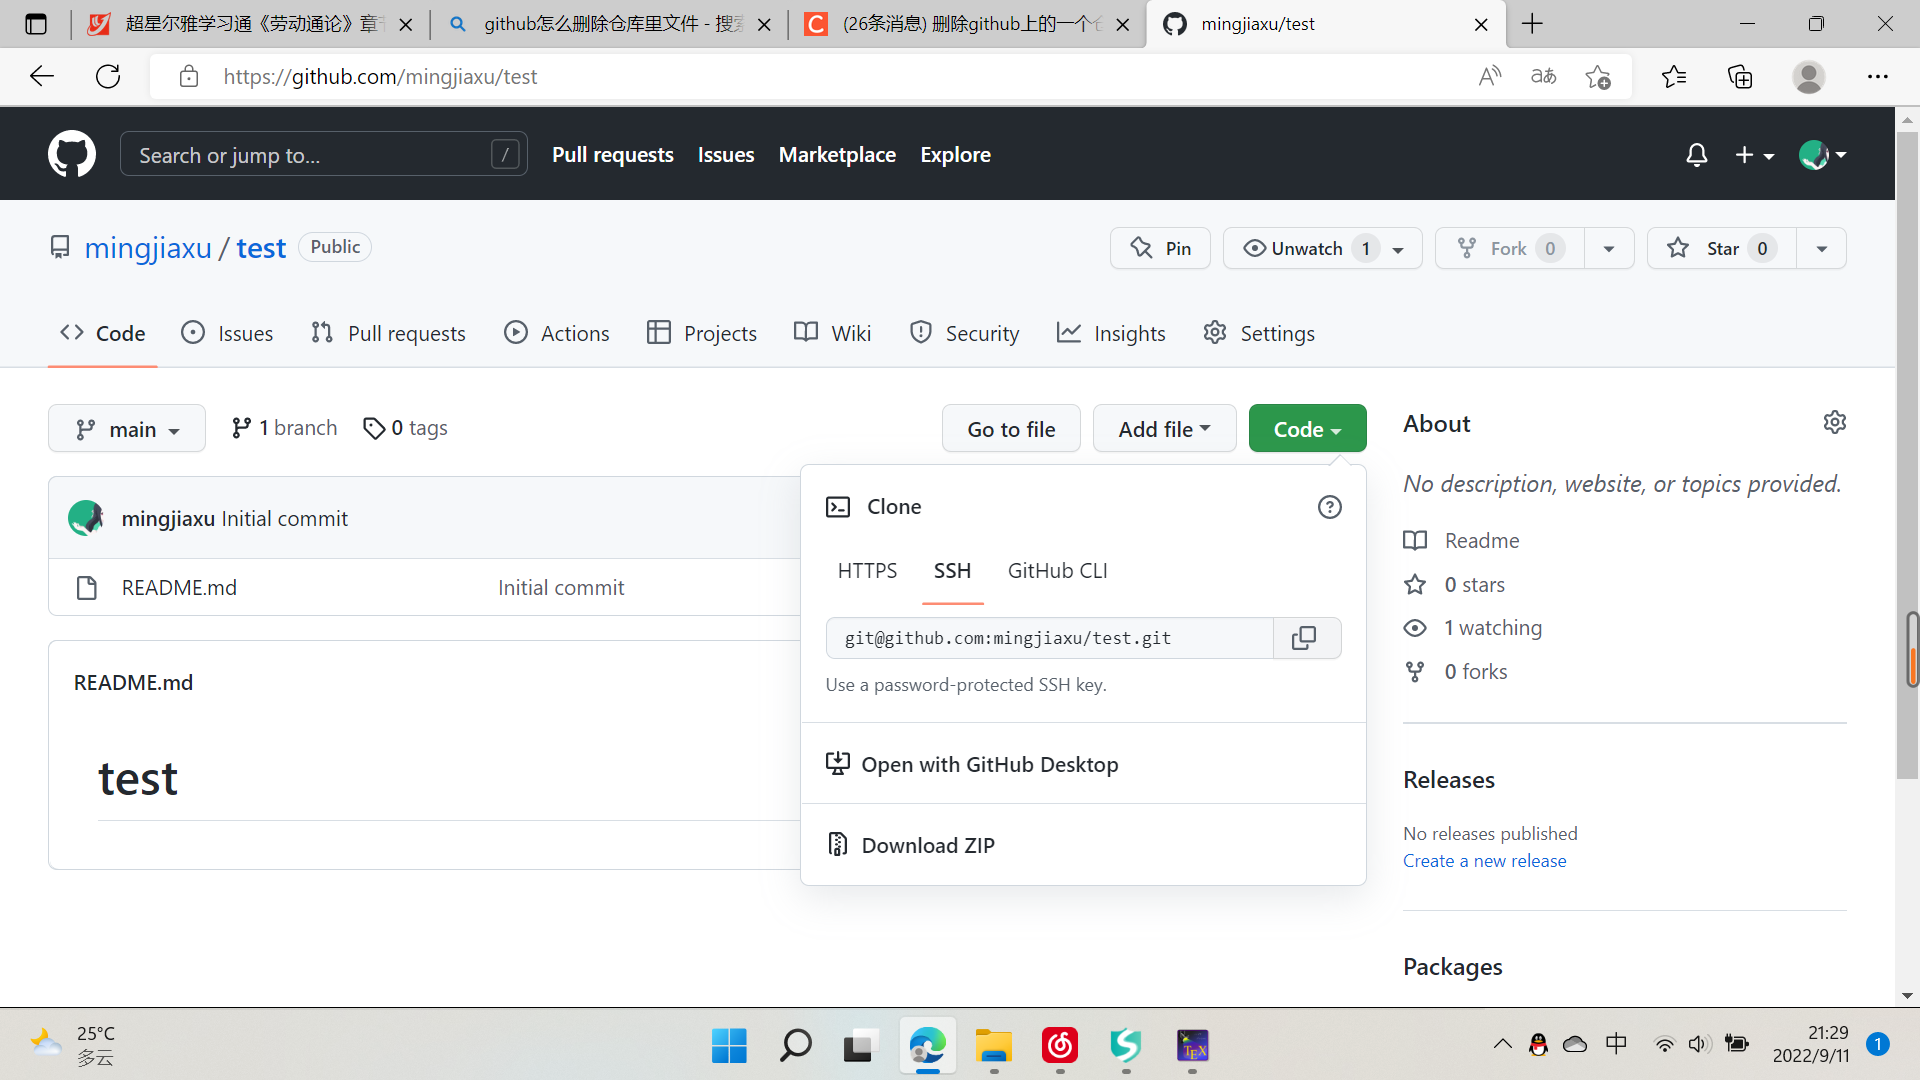
\includegraphics[width=5cm]{(4).png}
				\end{minipage}
			}
		\end{figure}
	\lstinputlisting[language=MATLAB]{code/command6.m}
	\subsection{在本地建立仓库,并上传文件} 		
		\begin{enumerate}
			\item 新建文件夹,打开文件夹后运行Git Bash,输入 Git init 命令进行初始化操作.
				\begin{figure}[htbp]
					\centering
					\subfigure{
						\begin{minipage}{4cm}
							\centering
							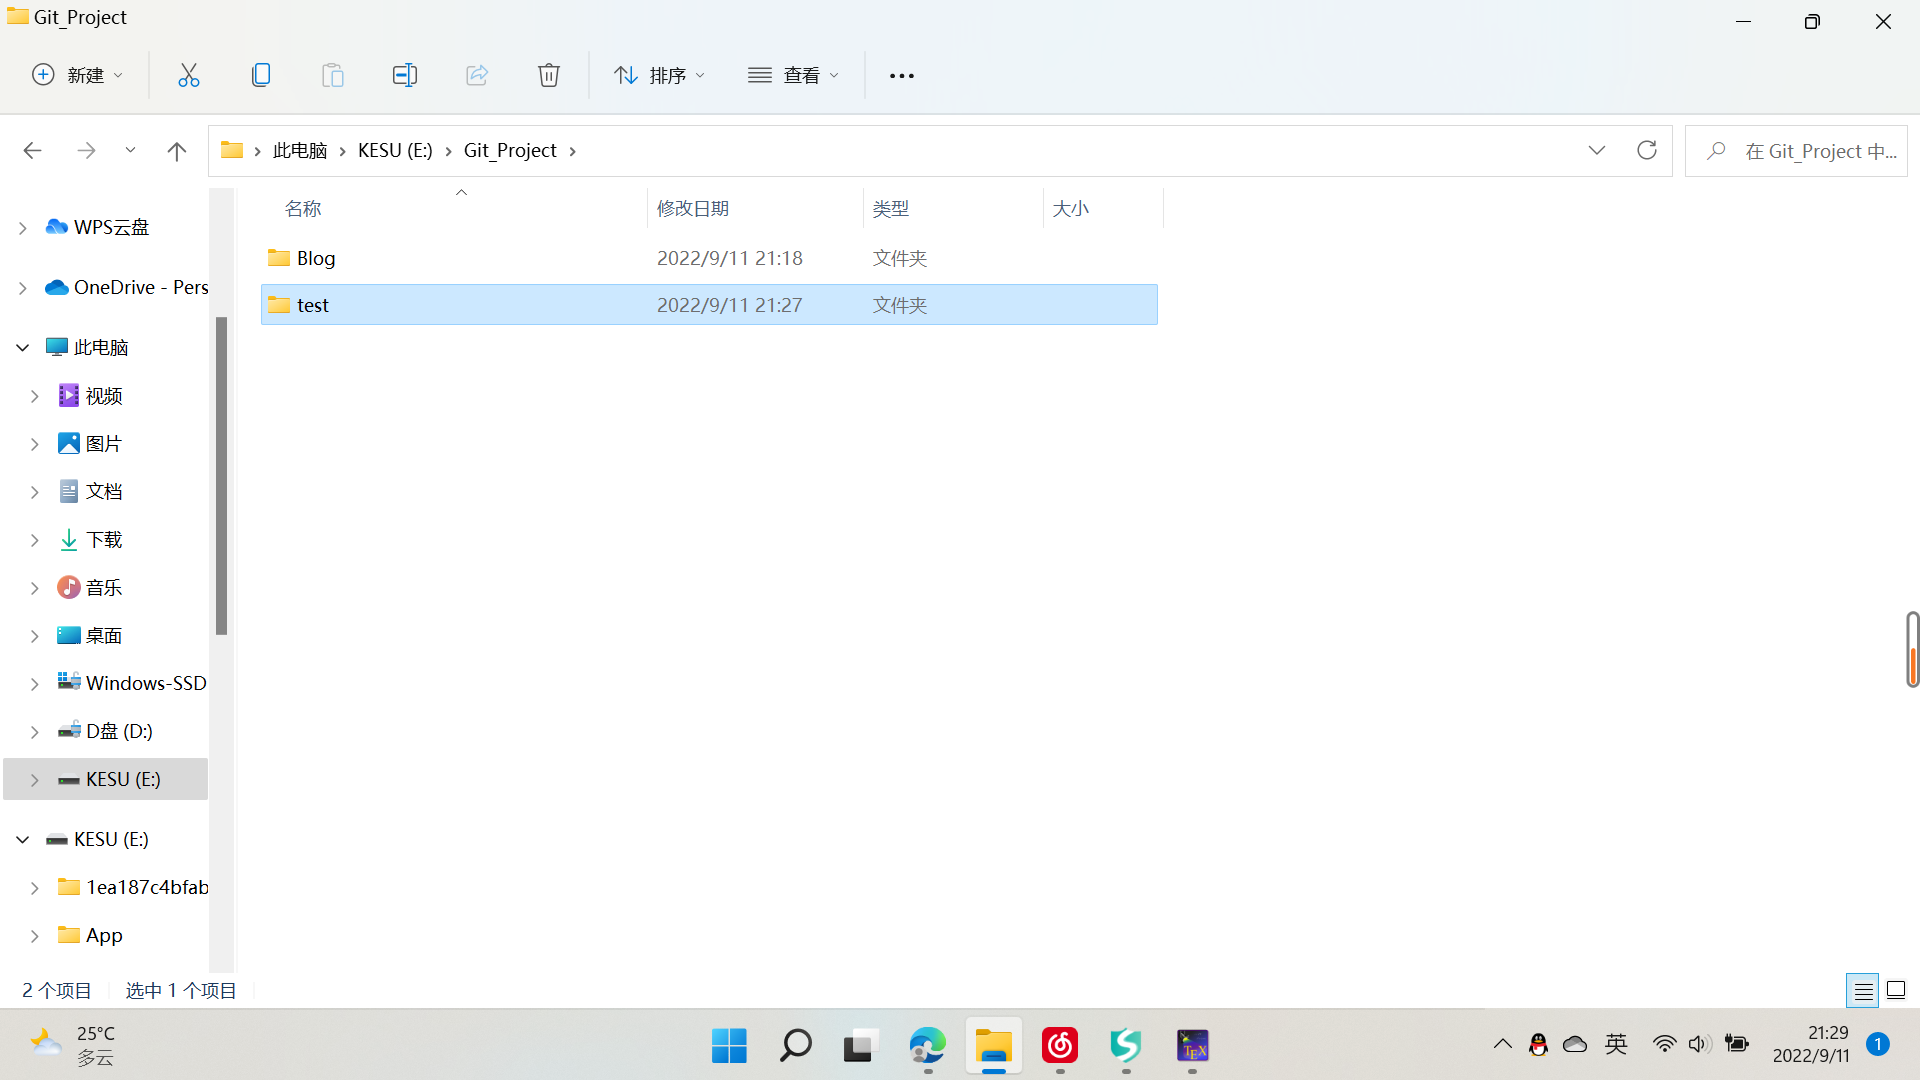
\includegraphics[width=3cm]{(5).png}
						\end{minipage}%
					}%
					\subfigure{
						\begin{minipage}{4cm}
							\centering
							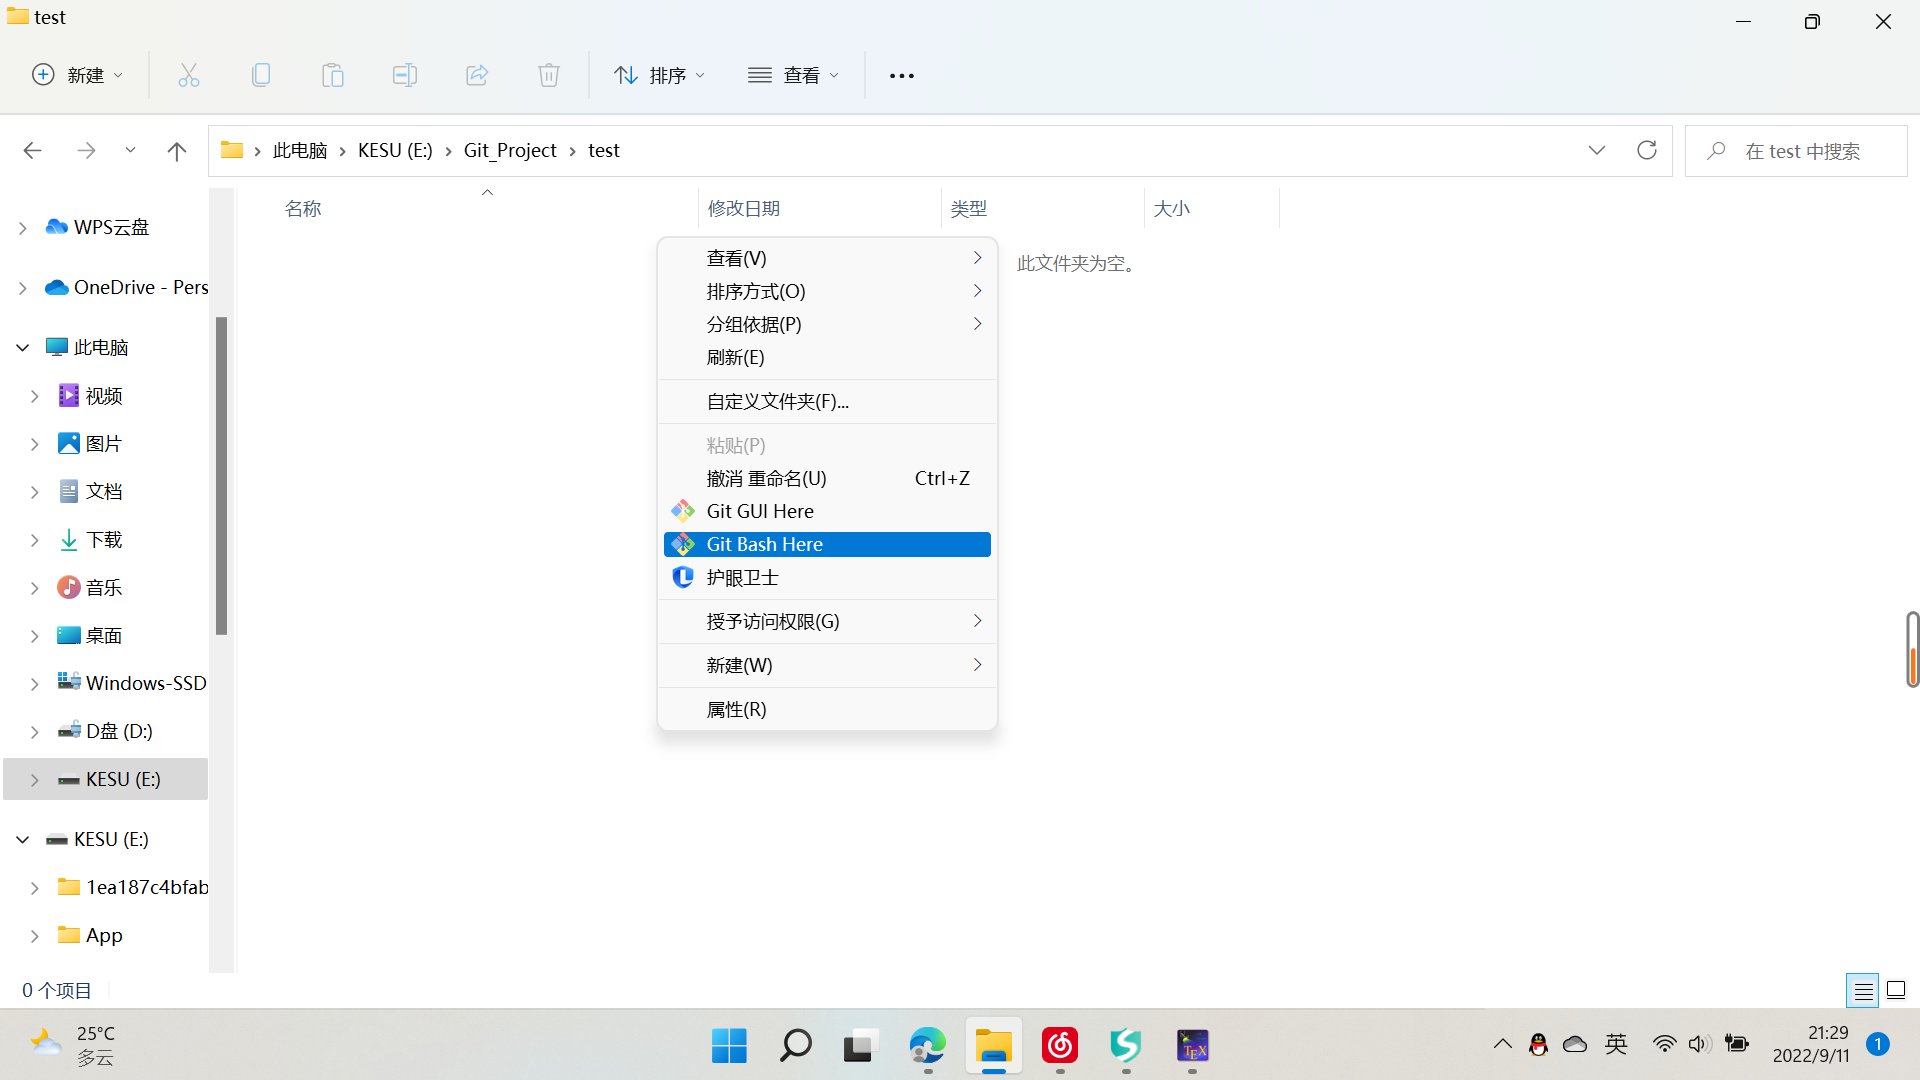
\includegraphics[width=3cm]{(19).png}
						\end{minipage}
					}
					\subfigure{
						\begin{minipage}{4cm}
							\centering
							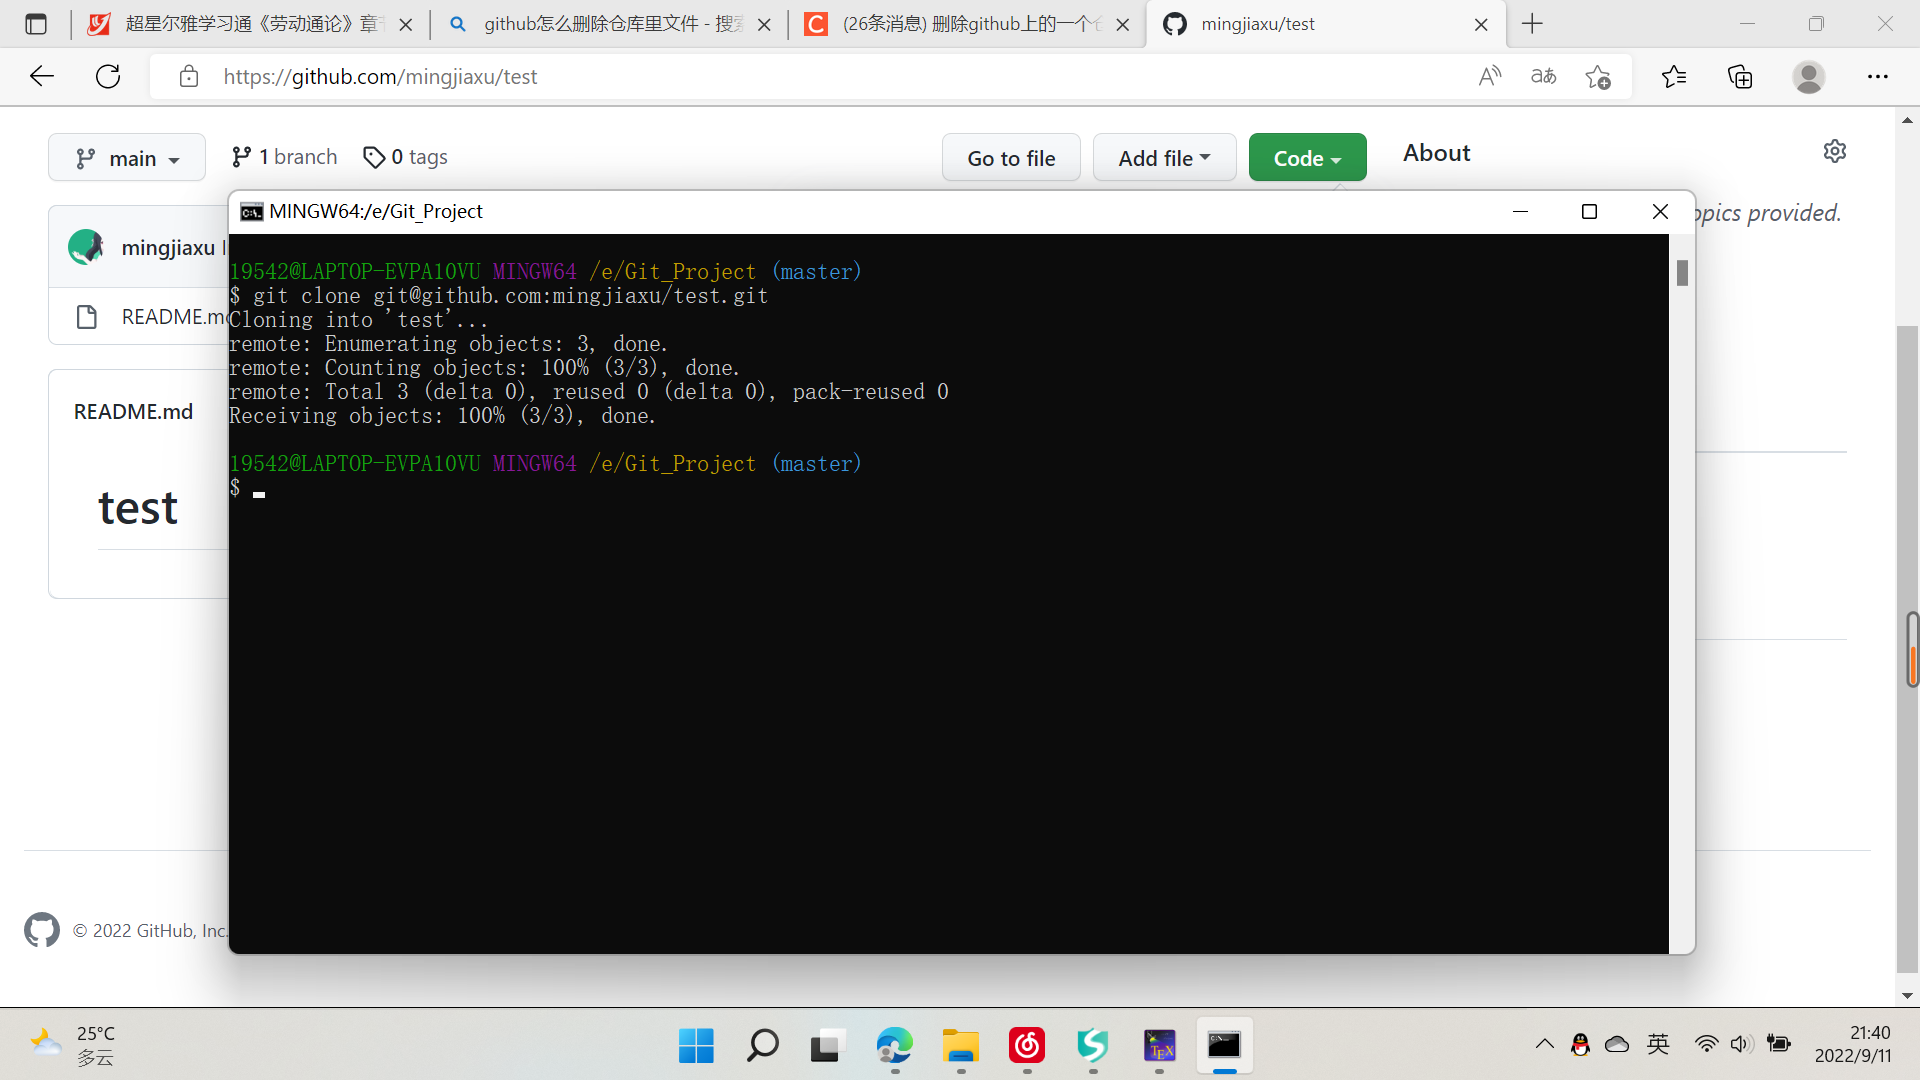
\includegraphics[width=3cm]{(6).png}
						\end{minipage}%
					}%
				\end{figure}
			\item{初始化完成后,运行Git clone 操作,将网站仓库克隆下来.} 
					\begin{figure}[htbp]
					\centering
					\subfigure{
						\begin{minipage}{4cm}
							\centering
							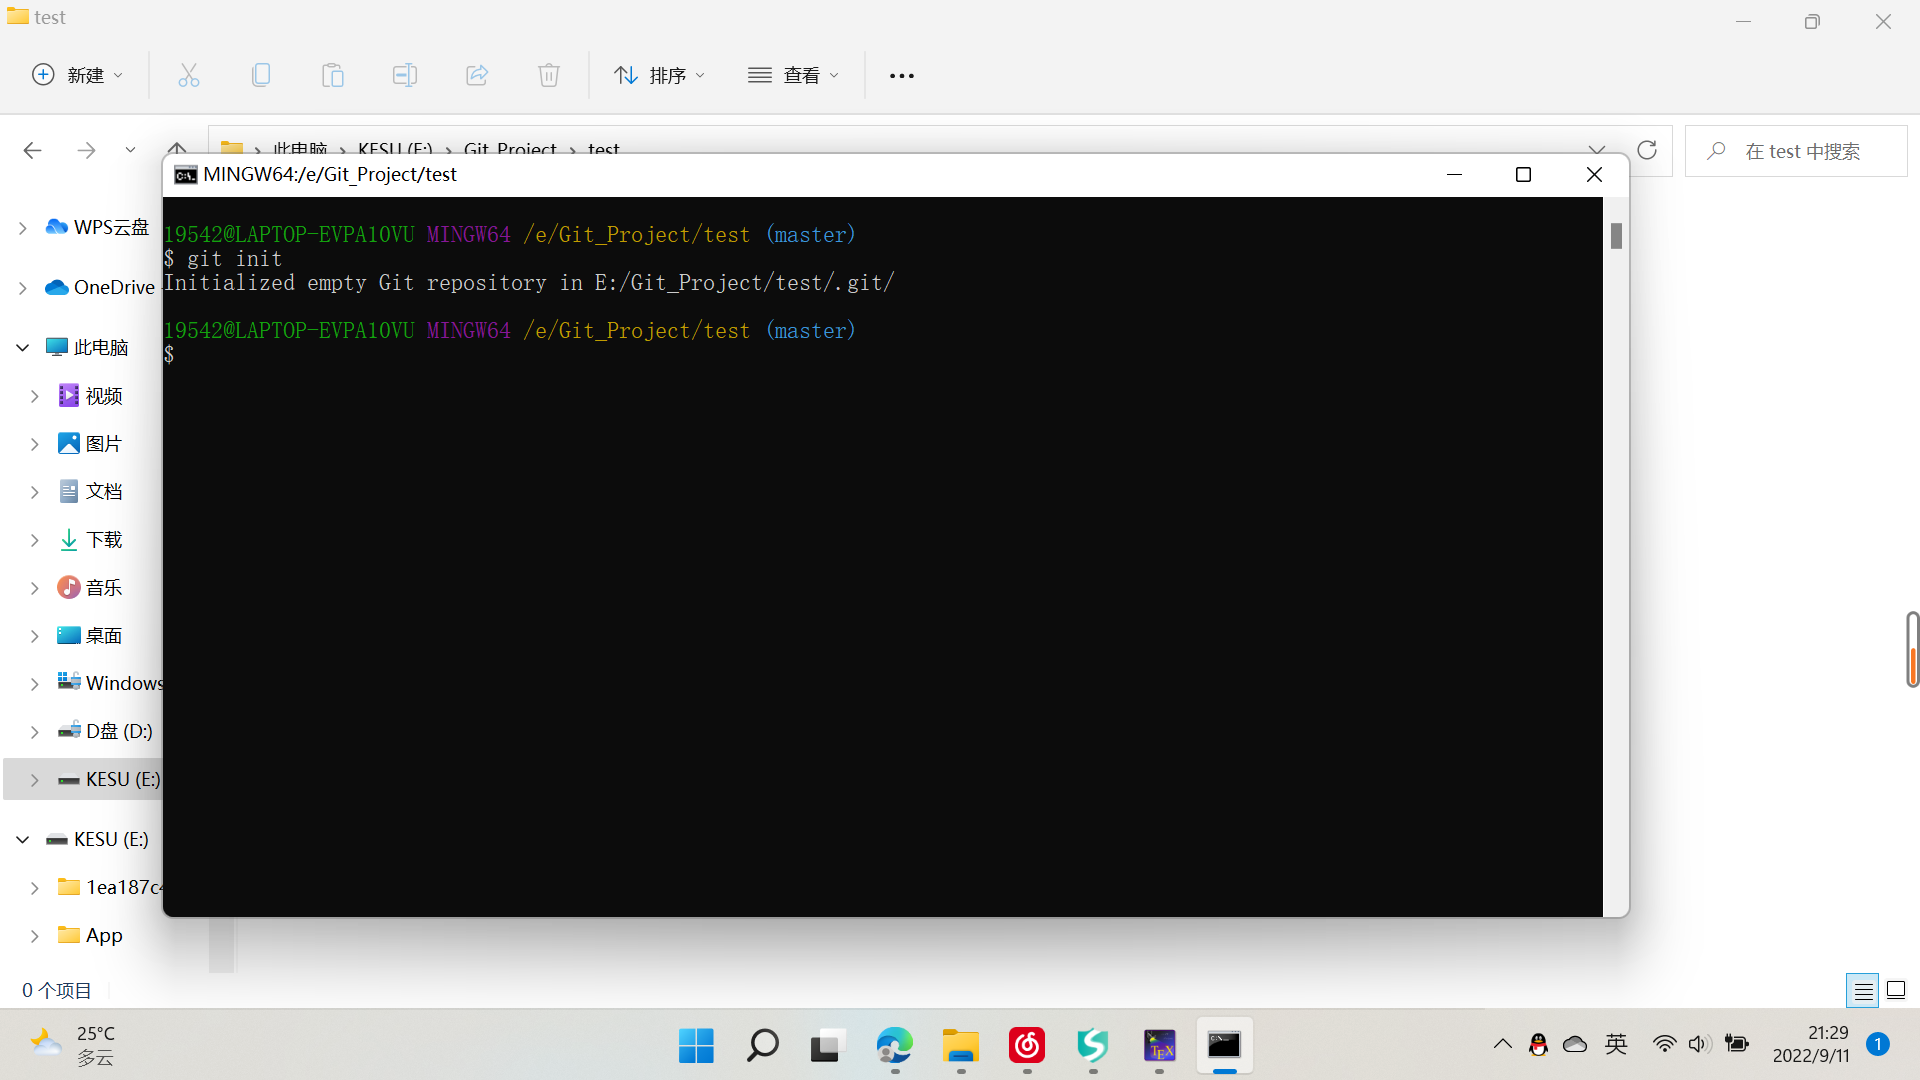
\includegraphics[width=3cm]{(20).png}
						\end{minipage}%
					}%
					\subfigure{
						\begin{minipage}{4cm}
							\centering
							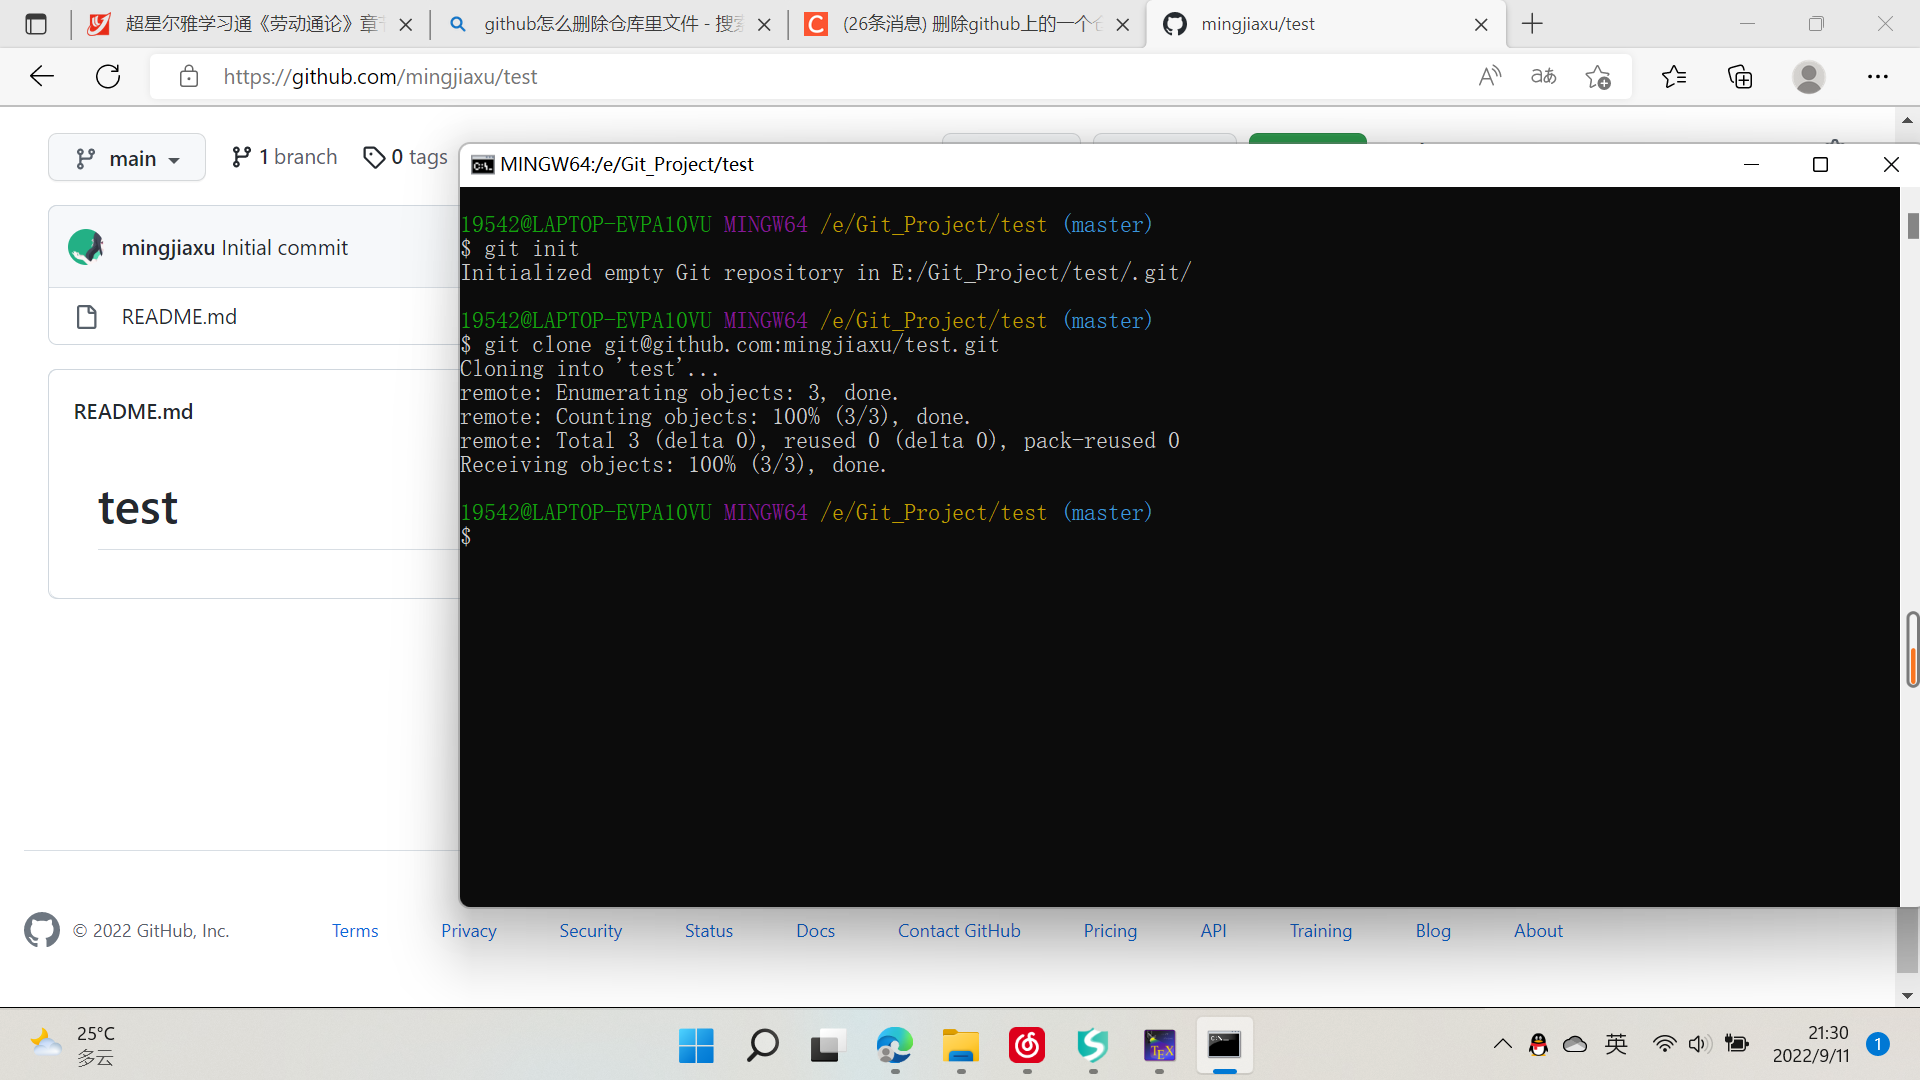
\includegraphics[width=3cm]{(21).png}
						\end{minipage}%
					}%
					\subfigure{
						\begin{minipage}{4cm}
							\centering
							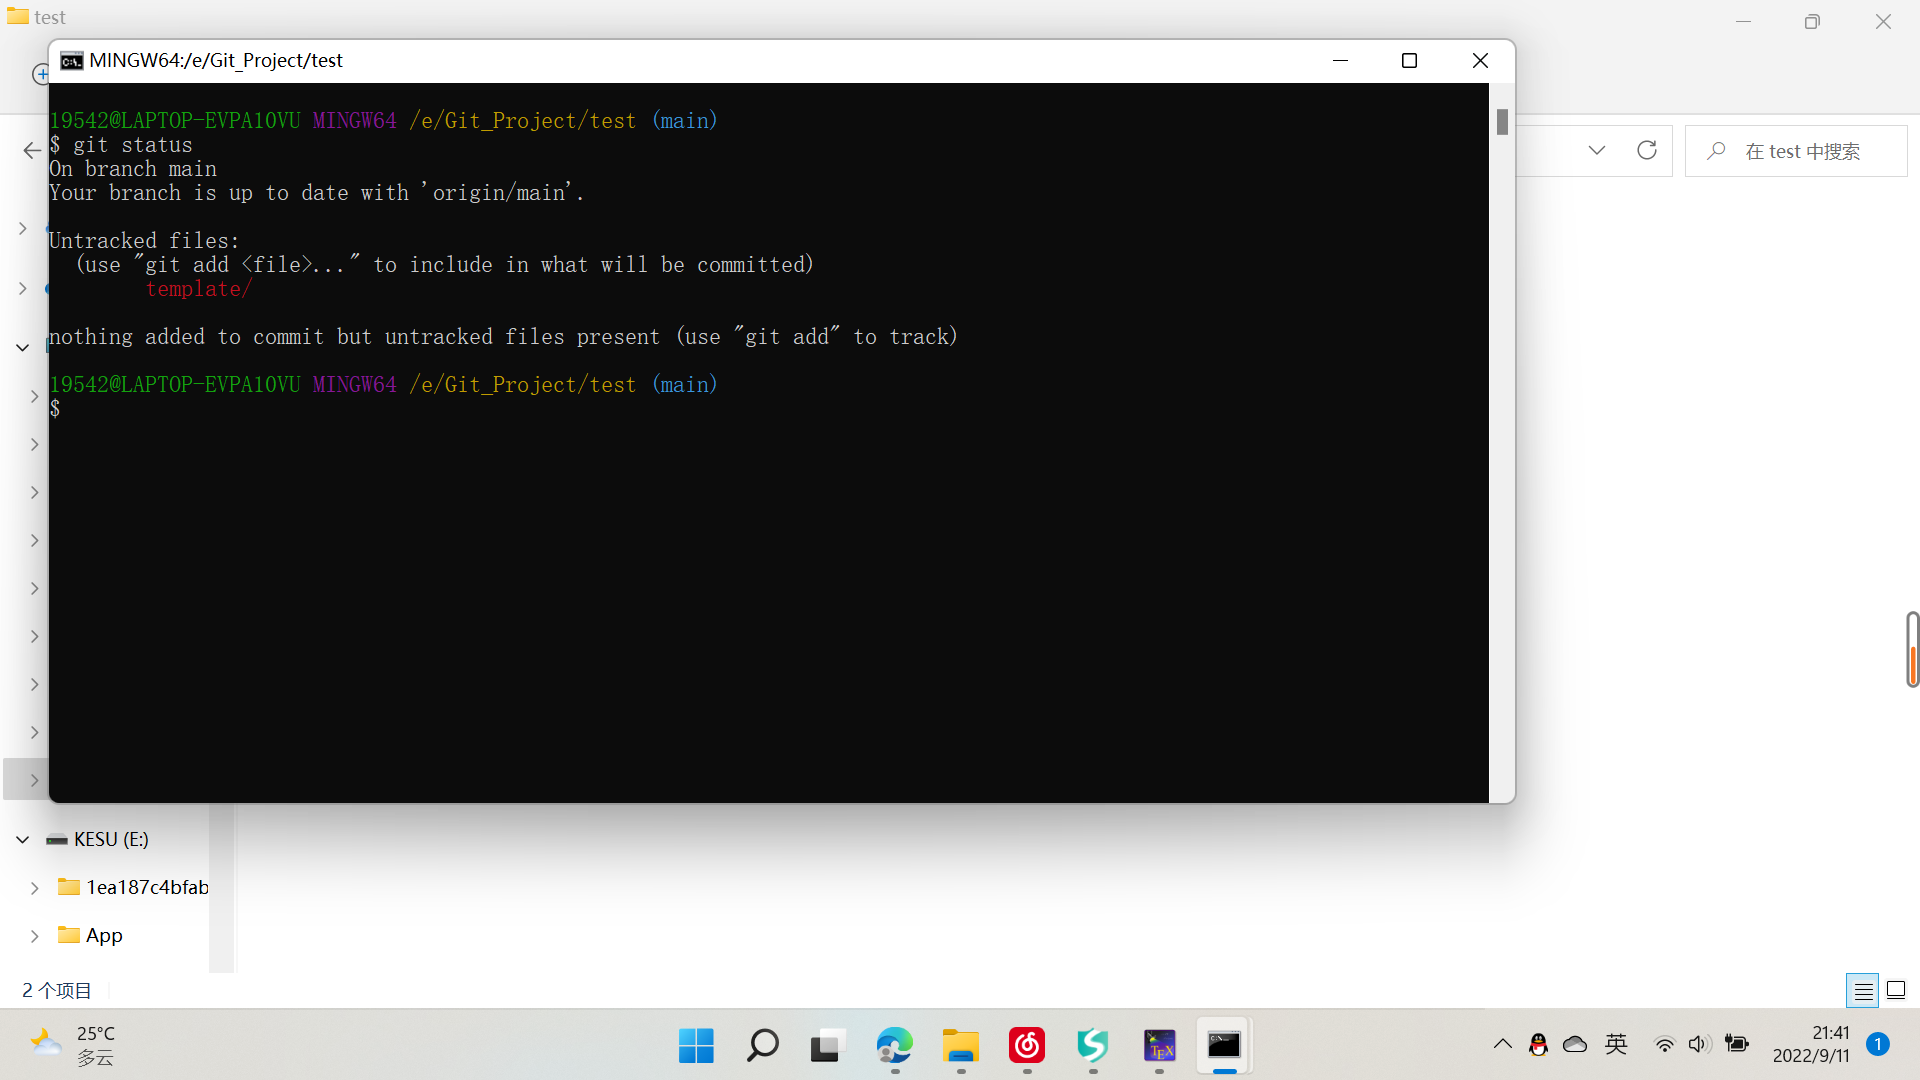
\includegraphics[width=3cm]{(10).png}
						\end{minipage}%
					}%
				\end{figure}
		\item{在test仓库内放入待上传文件,后运行给Git Bash,输入git status 查看状态.} 
		\begin{figure}[htbp]
			\centering
			\subfigure{
				\begin{minipage}{4cm}
					\centering
					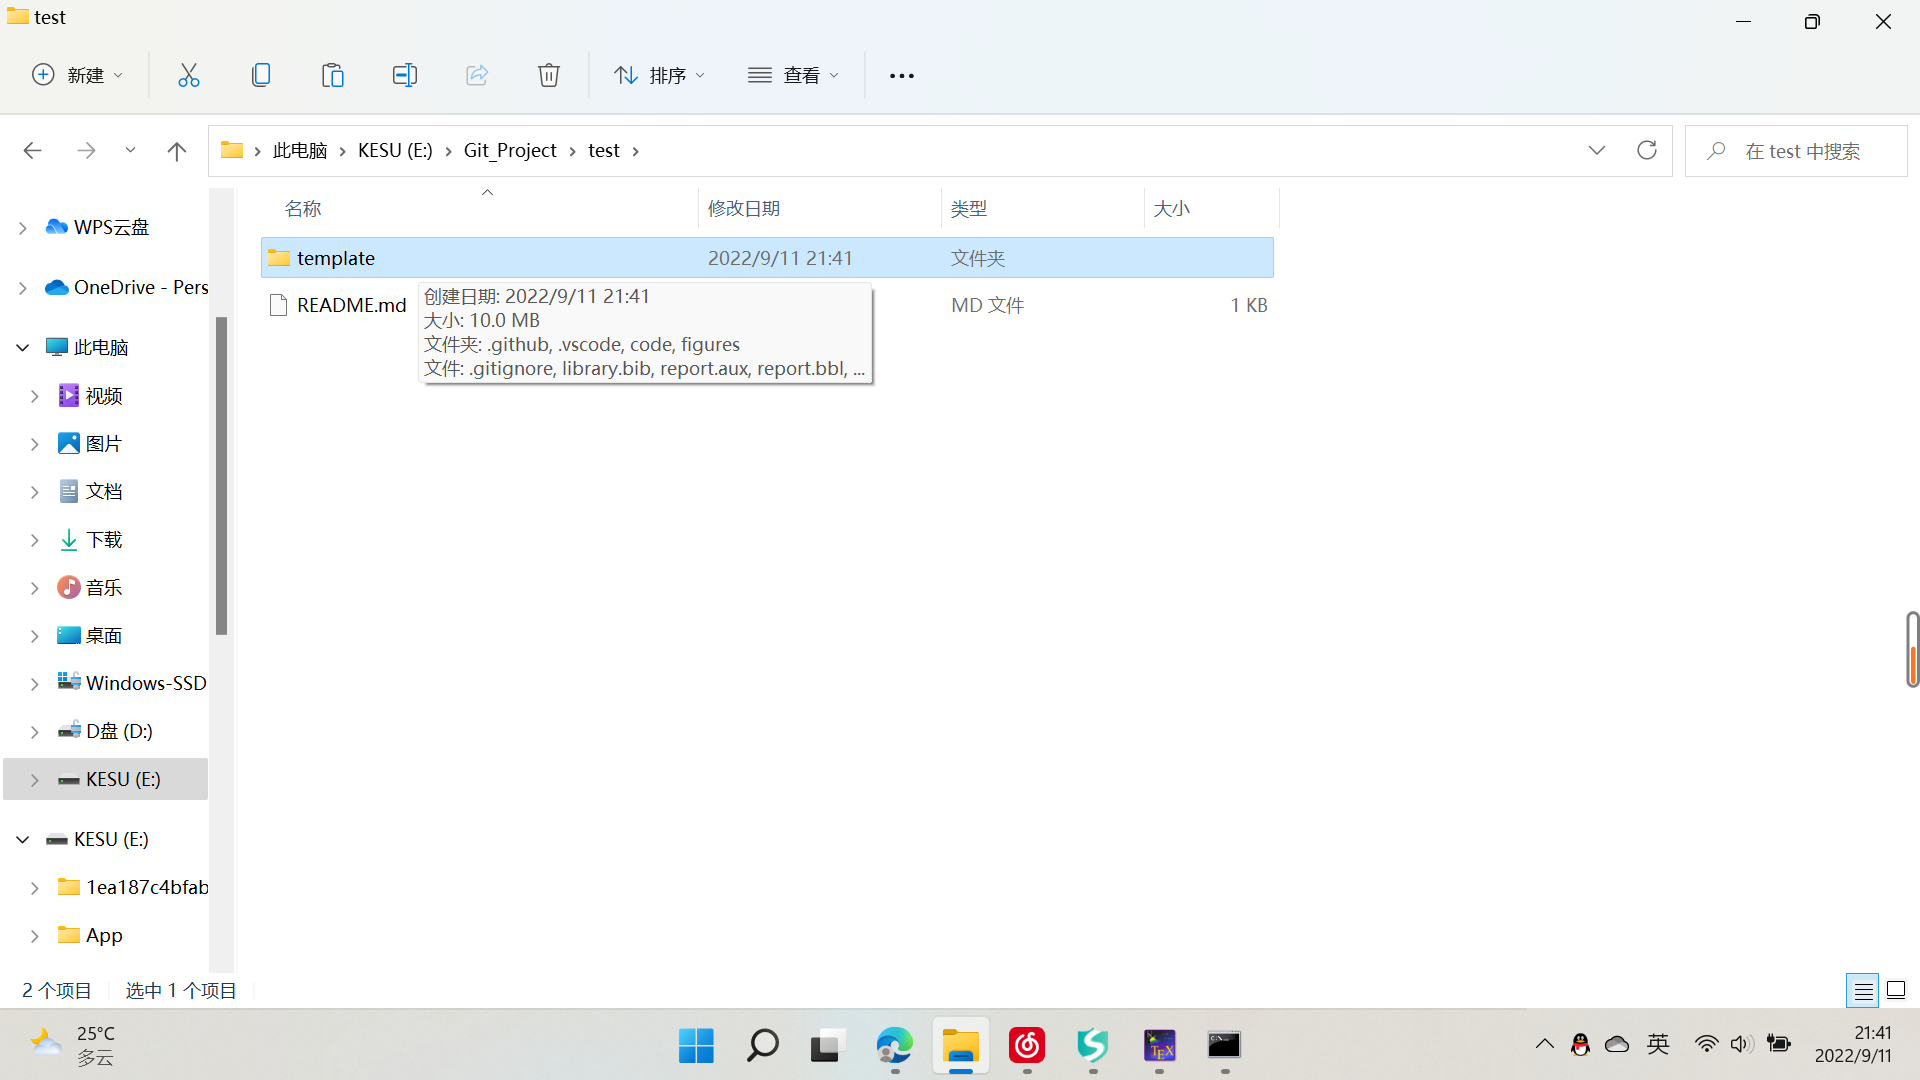
\includegraphics[width=3cm]{(8).png}
				\end{minipage}
			}
			\subfigure{
				\begin{minipage}{4cm}
					\centering
					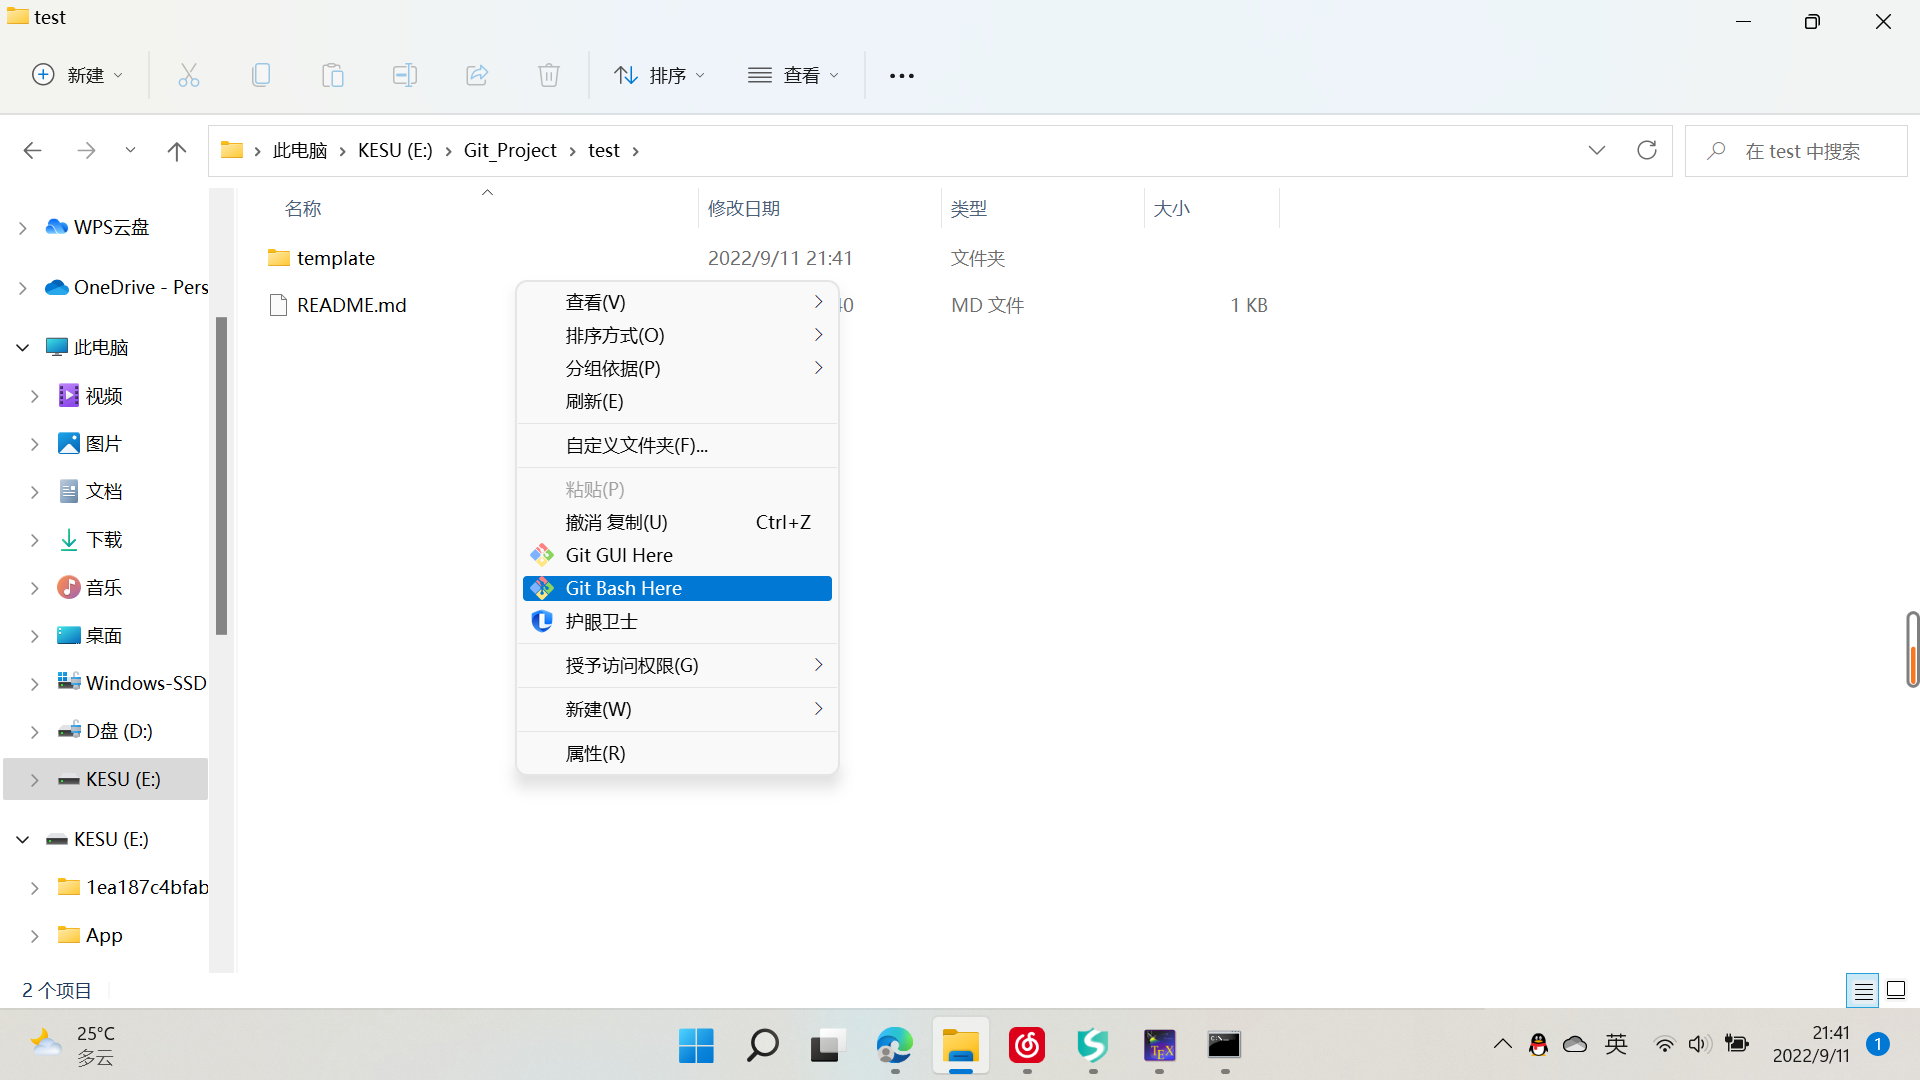
\includegraphics[width=3cm]{(9).png}
				\end{minipage}
			}
			\subfigure{
				\begin{minipage}{4cm}
					\centering
					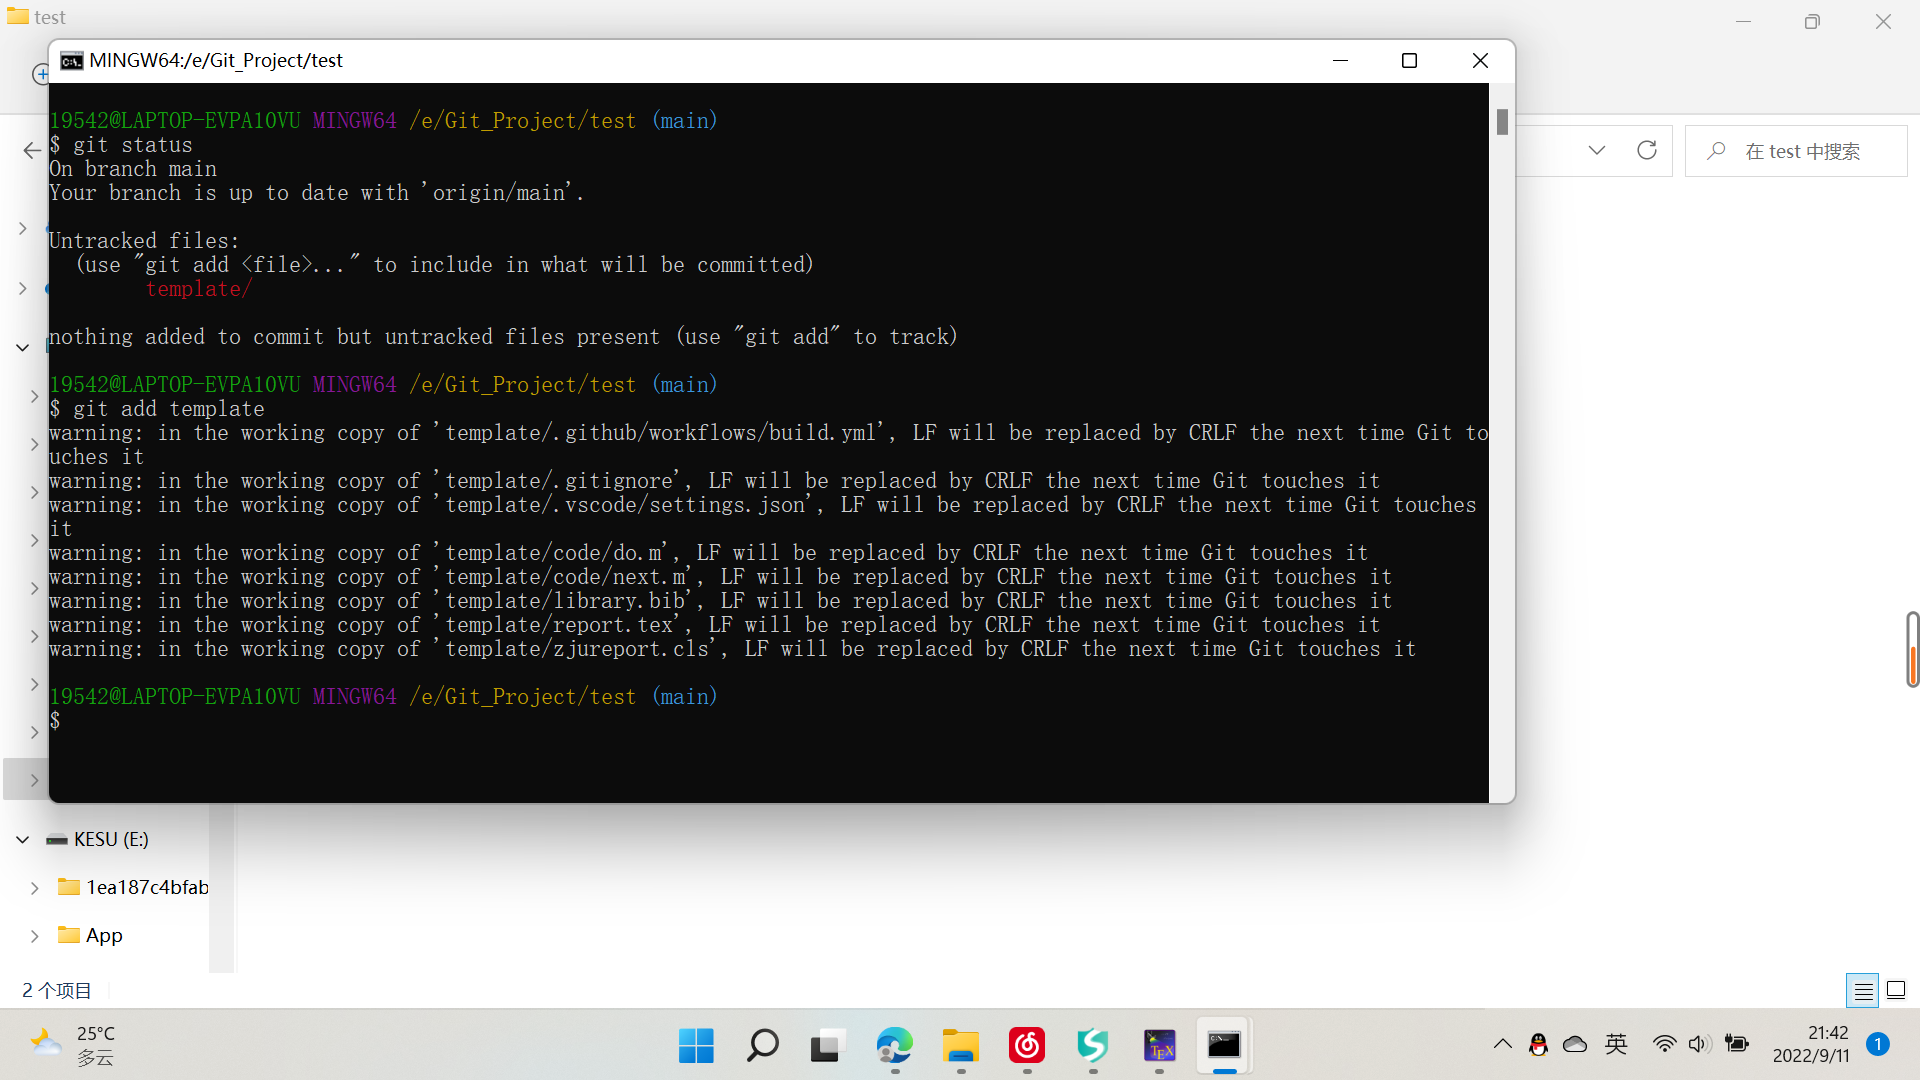
\includegraphics[width=3cm]{(11).png}
				\end{minipage}
			}
		\end{figure}
		\item 后输入 git add * 将文件添加,后用Git commit 提交文件.
			\begin{figure}[htbp]
			\centering
			\subfigure{
				\begin{minipage}{4cm}
					\centering
					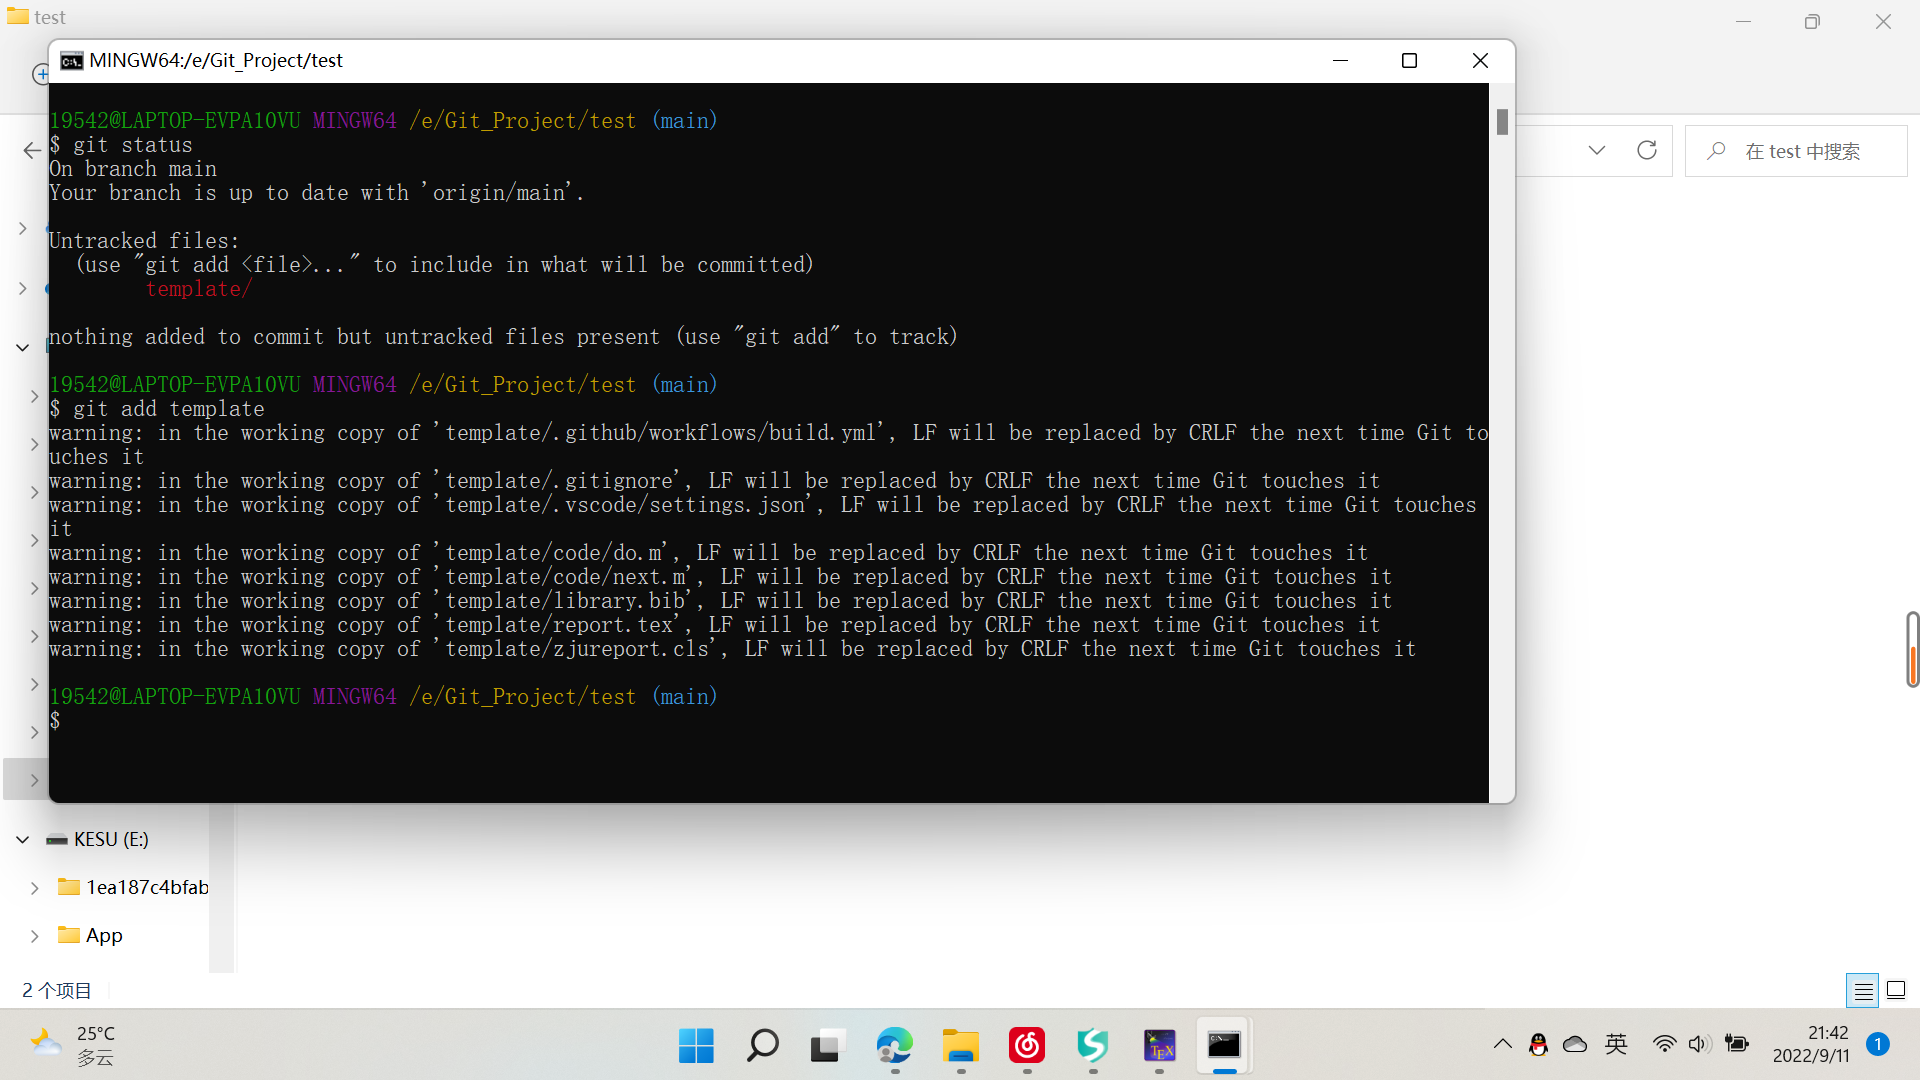
\includegraphics[width=3cm]{(11).png}
				\end{minipage}
			}
			\subfigure{
				\begin{minipage}{4cm}
					\centering
					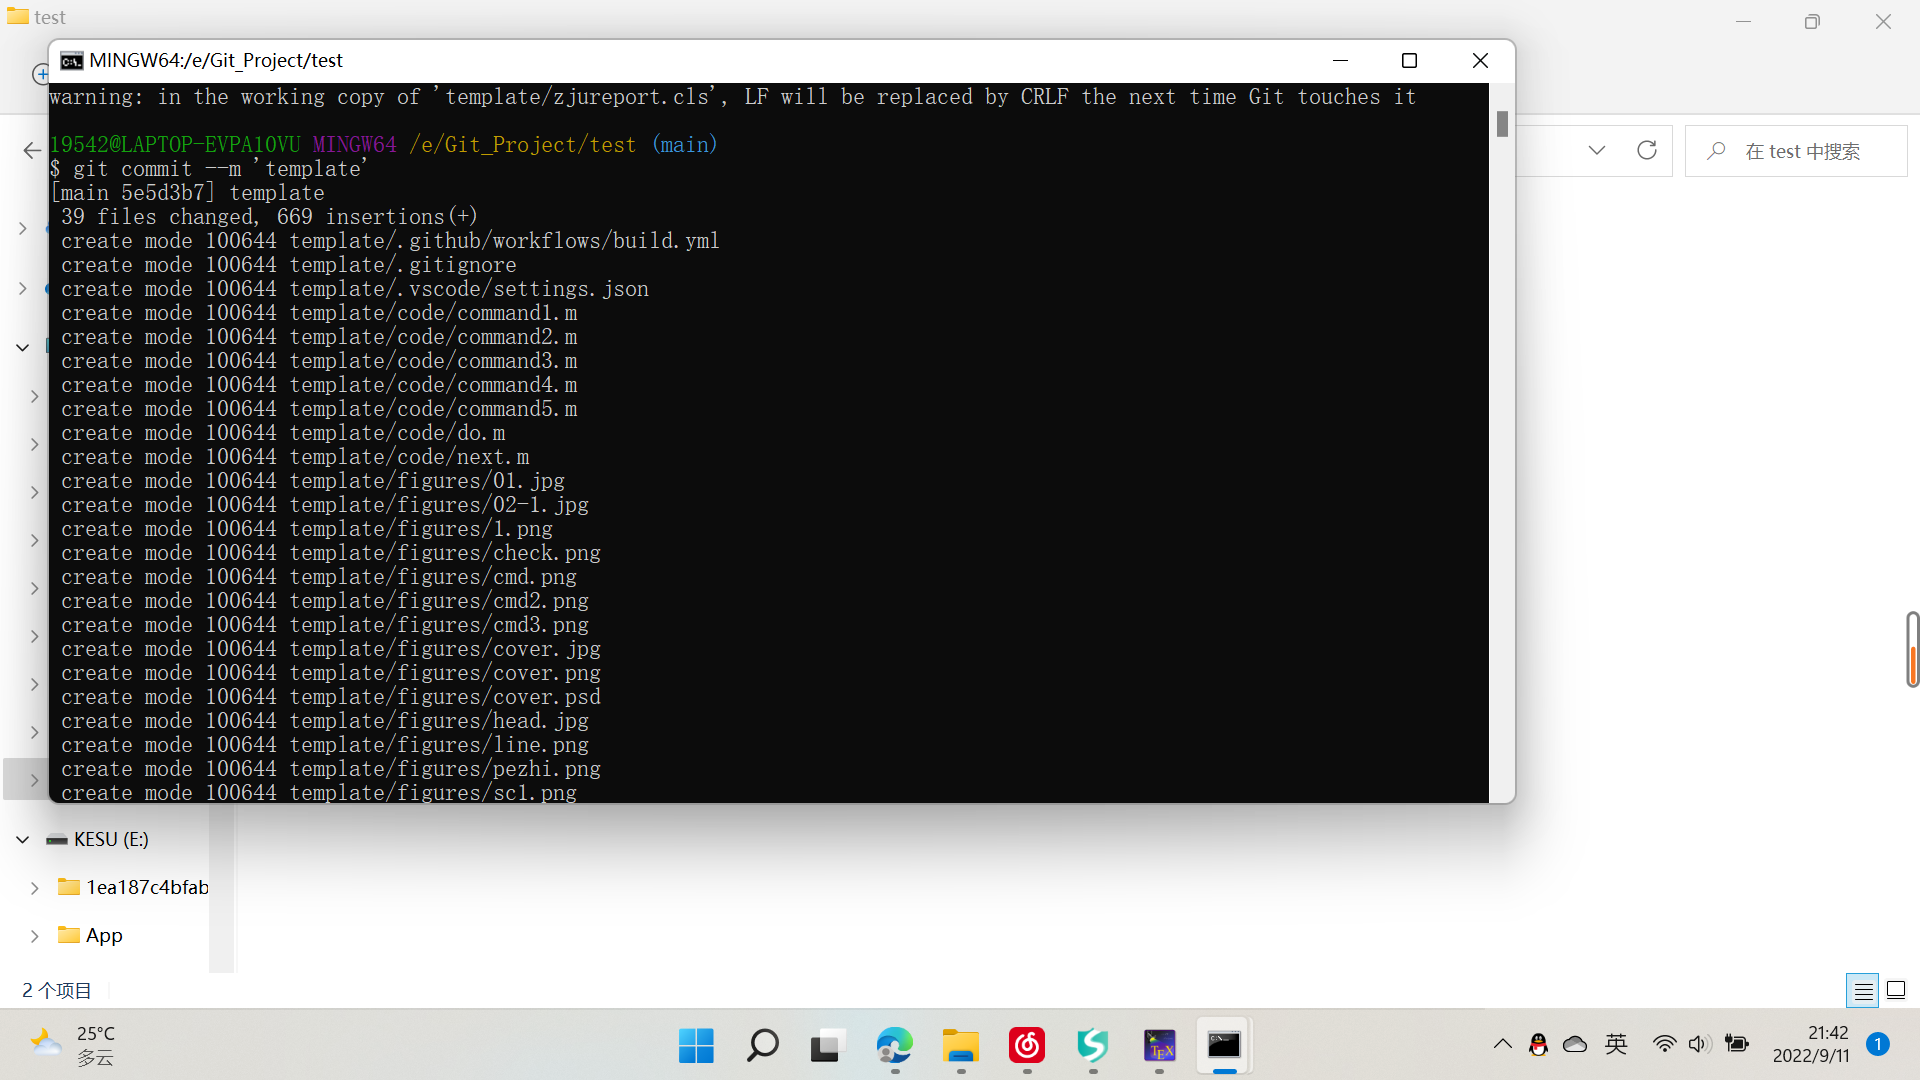
\includegraphics[width=3cm]{(12).png}
				\end{minipage}
			}
			\subfigure{
				\begin{minipage}{4cm}
					\centering
					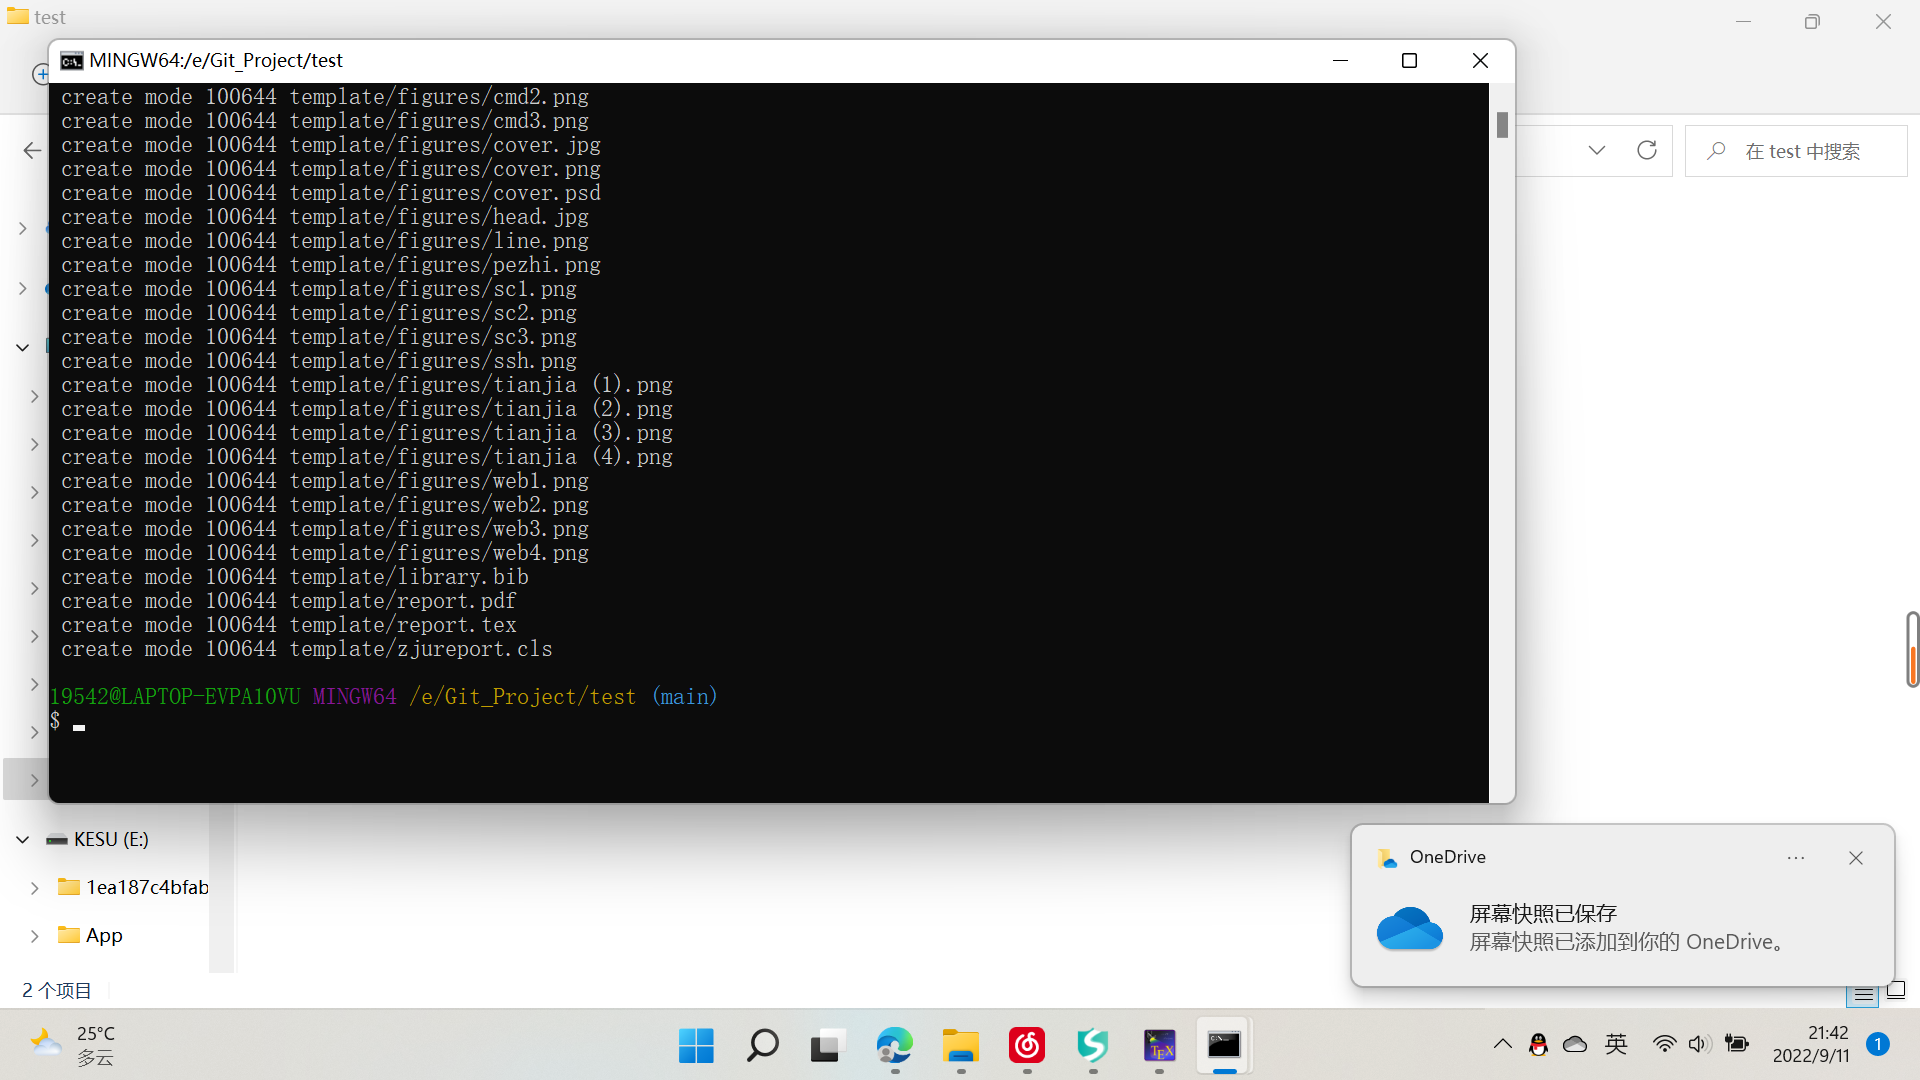
\includegraphics[width=3cm]{(13).png}
				\end{minipage}
			}
			\end{figure}
		\item 最后用 git push 将文件上传至网站.
			\begin{figure}[!htbp]
				\centering
				\subfigure{
				\begin{minipage}{4cm}
					\centering
					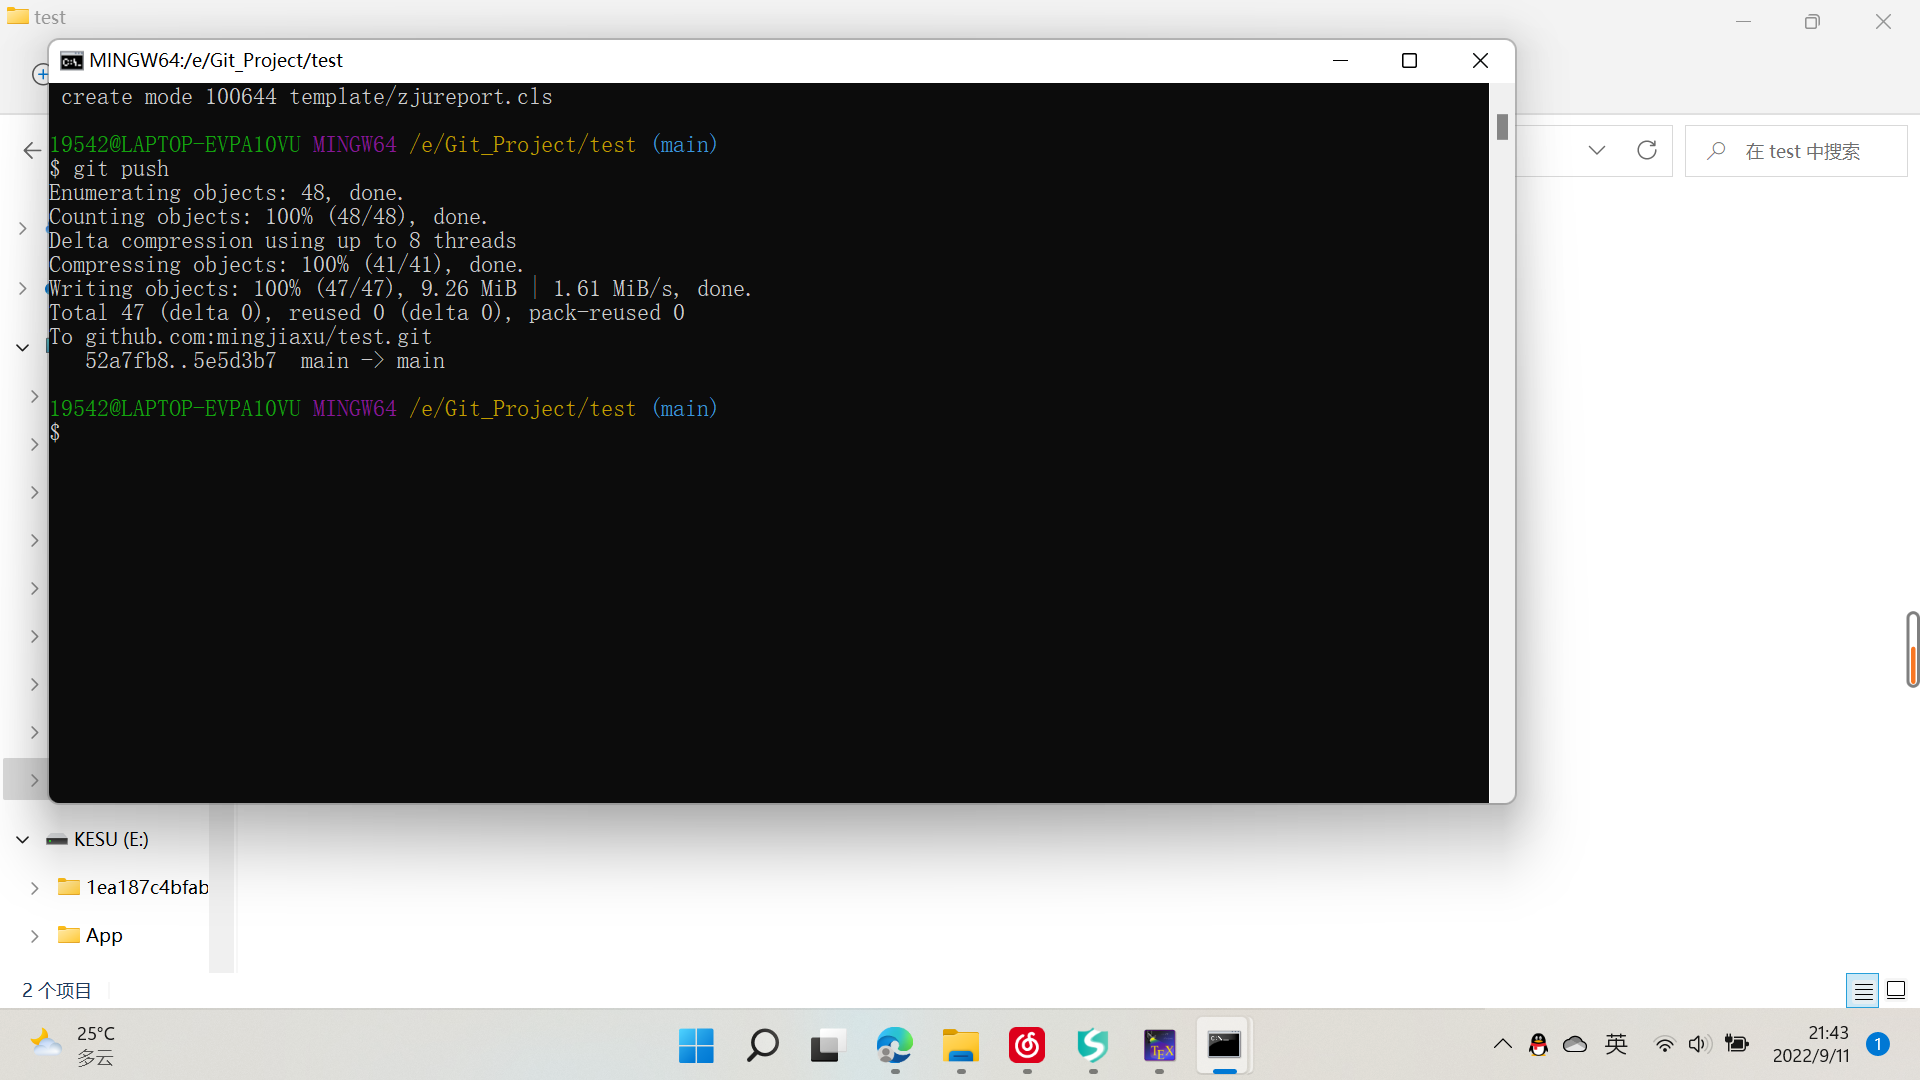
\includegraphics[width=3cm]{(14).png}
				\end{minipage}
				}
			\subfigure{
				\begin{minipage}{4cm}
					\centering
					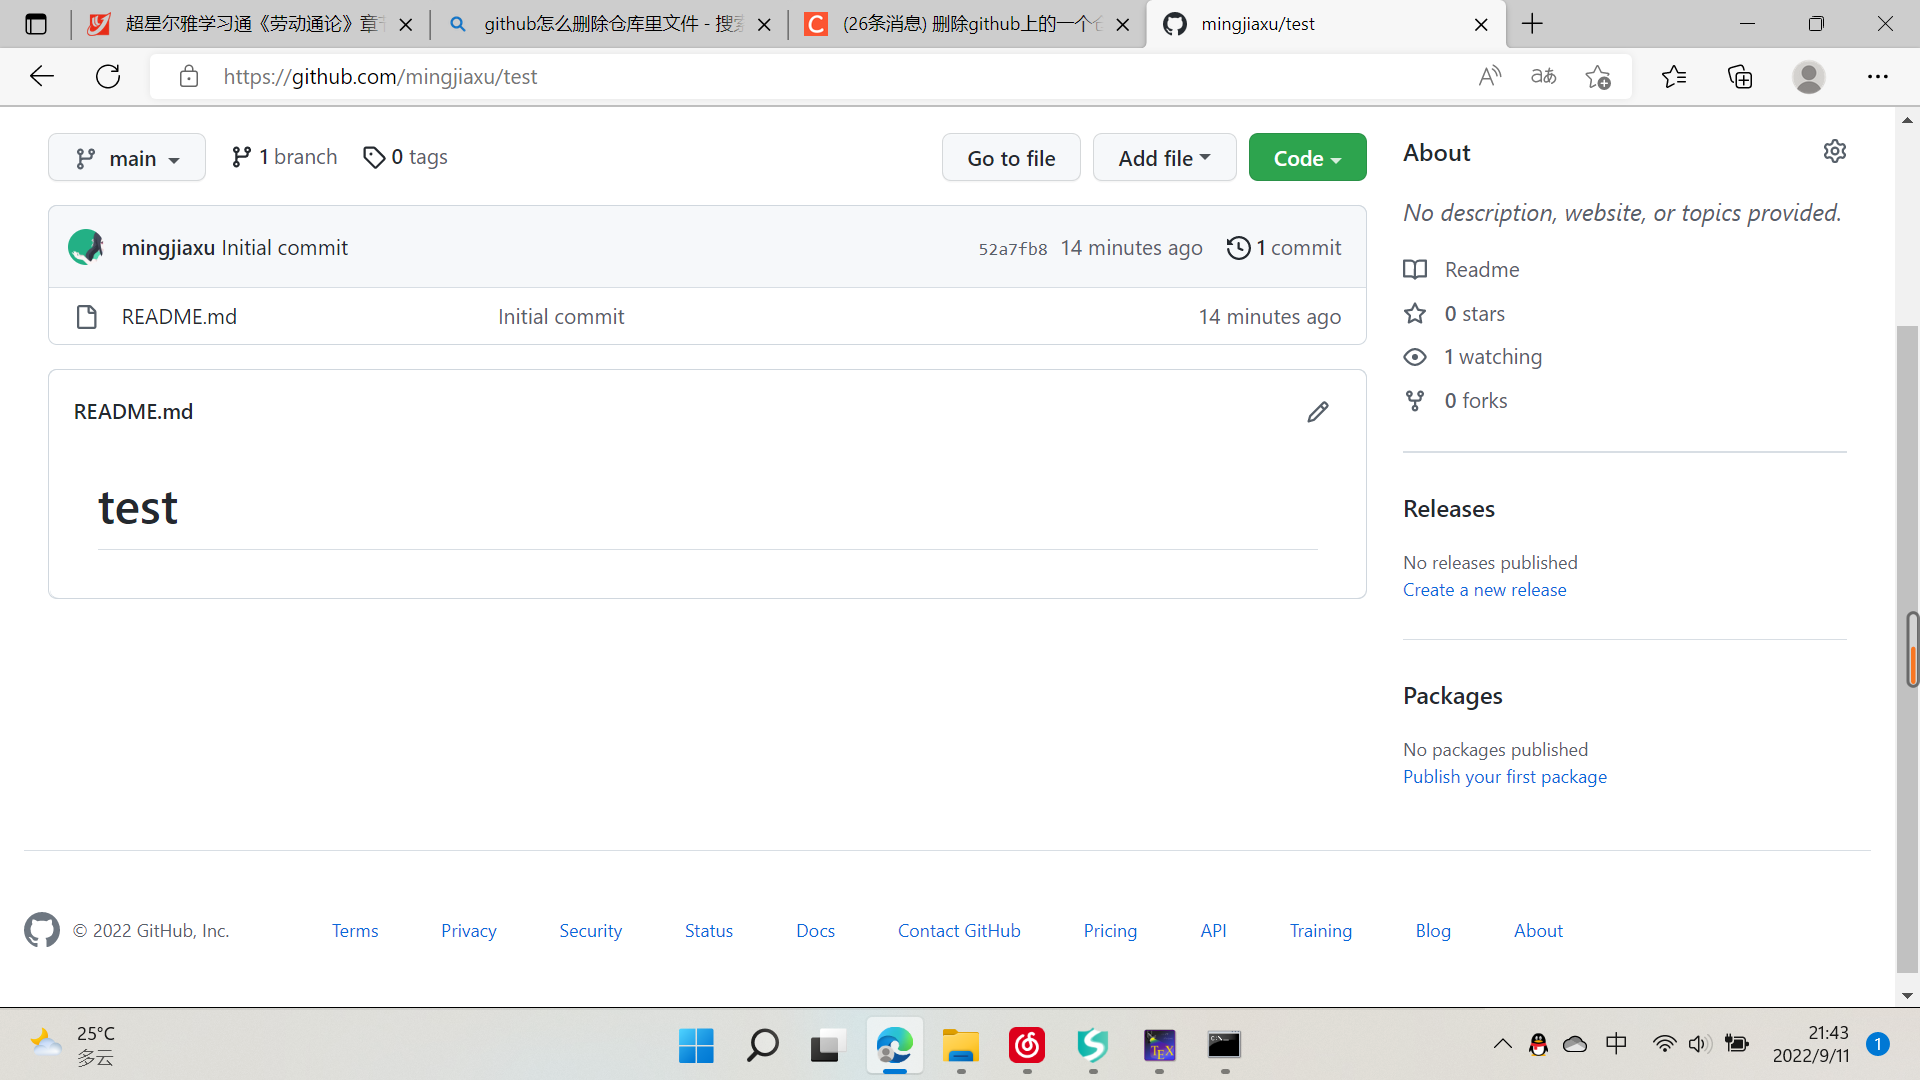
\includegraphics[width=3cm]{(16).png}
				\end{minipage}
			}
			\subfigure{
				\begin{minipage}{4cm}
					\centering
					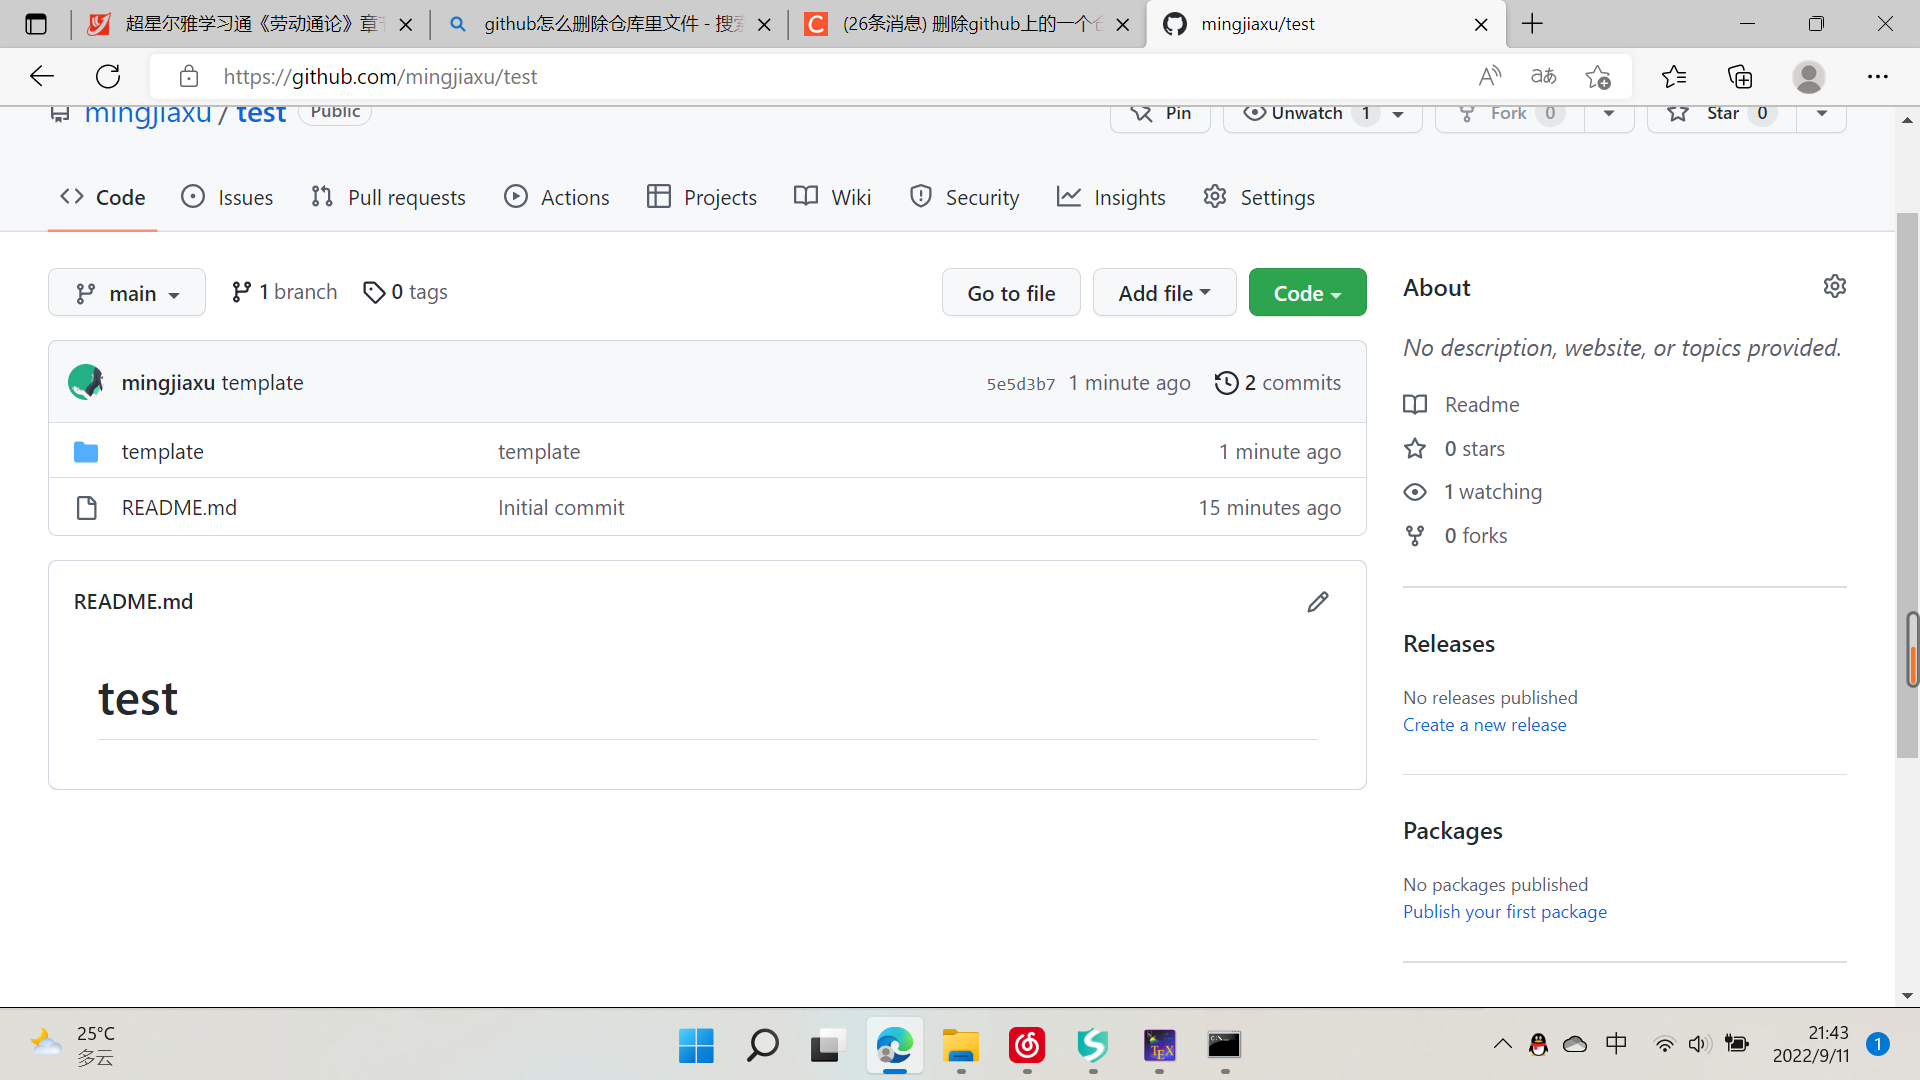
\includegraphics[width=3cm]{(17).png}
				\end{minipage}
			}
		\end{figure}
		\lstinputlisting[language=MATLAB]{code/command7.m}
	\end{enumerate}
\section{vscode配置python开发环境}
	安装python3.7,在系统环境变量中添加python的exe可执行文件路径,于vscode下载python extension 插件,vscode配置python开发环境完成,后通过pip命令安装numpy、matplotlib、PYQT5及其相关模块,值得注意的的是Qtdesigner的exe可执行文件路径同样需要添加至系统环境变量,同时按住安装对应插件,这样才能在vscode中快速使用QTdesigner,若不添加至环境变量,该插件无法找到对应路径,将无法打开。
	\begin{figure}[htbp]
		\centering
		\subfigure{
			\begin{minipage}{5cm}
				\centering
				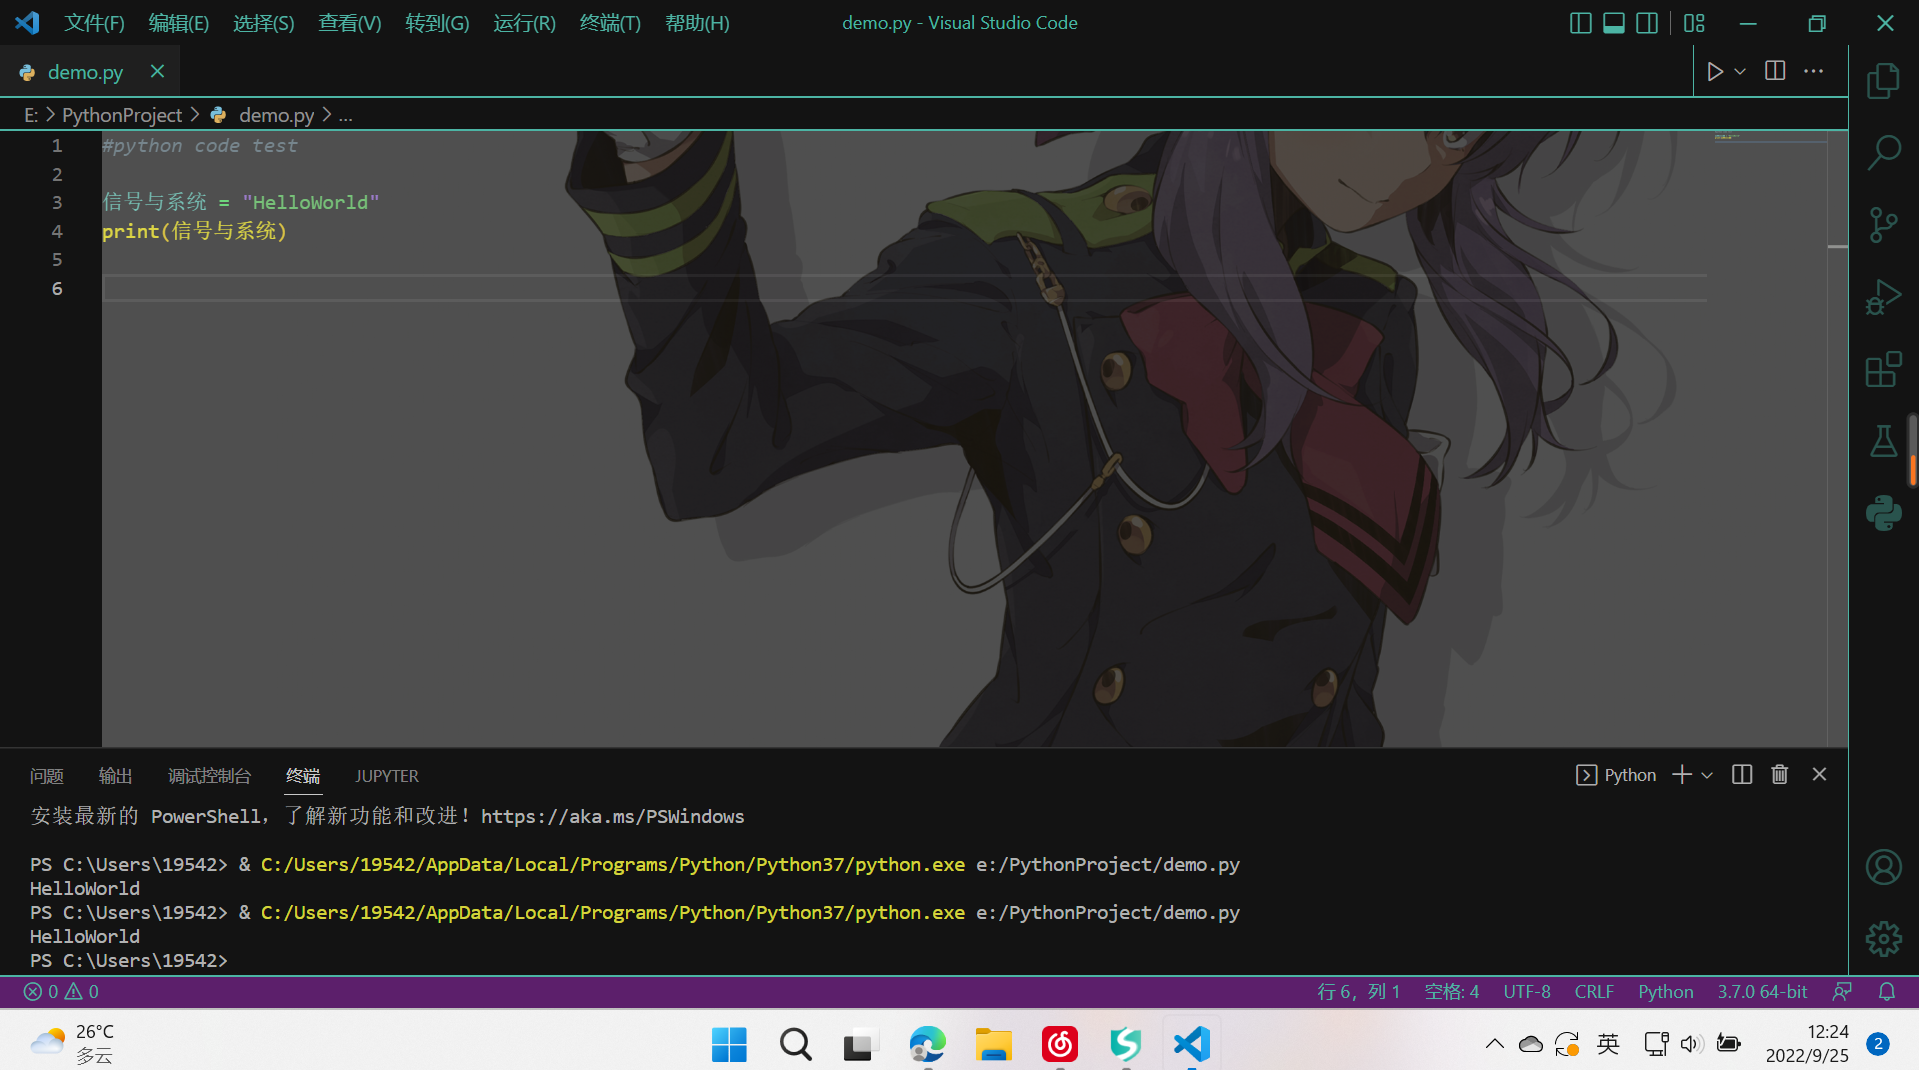
\includegraphics[width=5cm]{1 (2).png}
			\end{minipage}
		}
		\subfigure{
			\begin{minipage}{5cm}
				\centering
				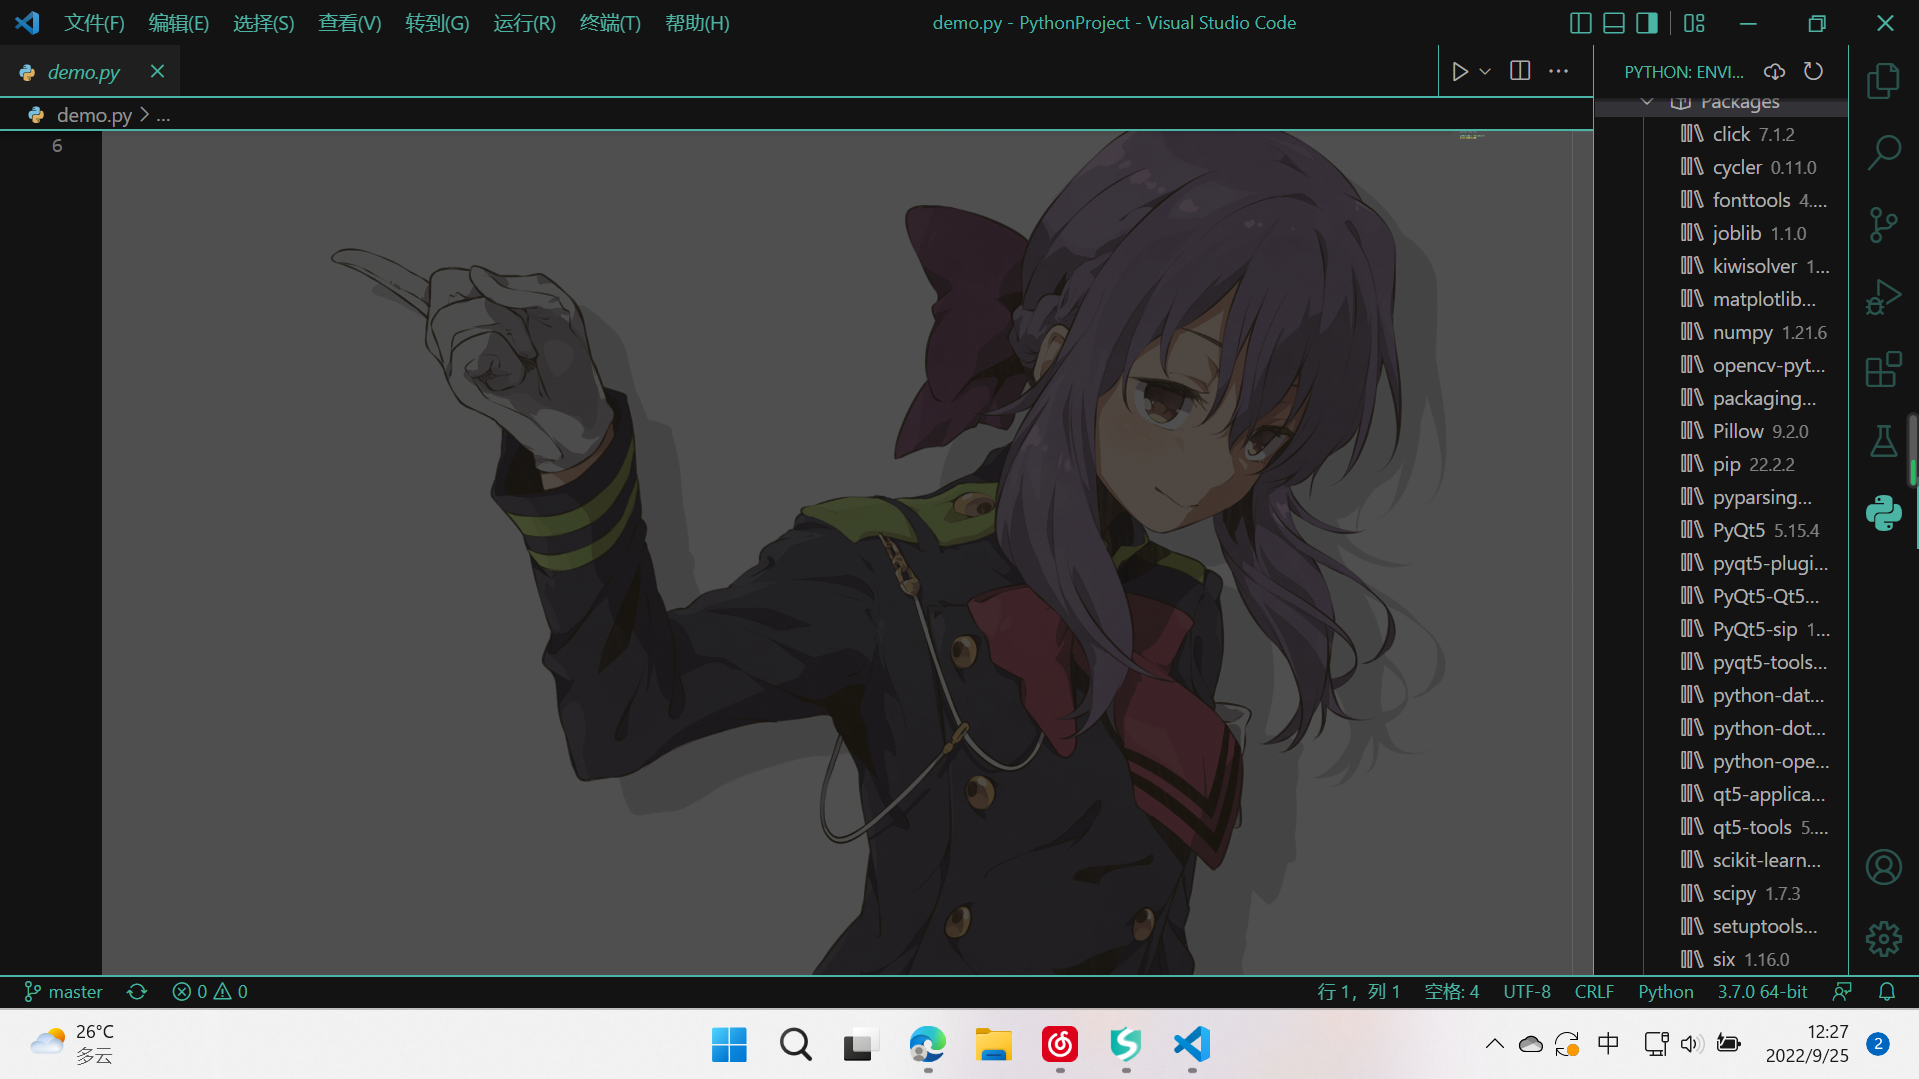
\includegraphics[width=5cm]{1 (8).png}
			\end{minipage}
		}
		\subfigure{
			\begin{minipage}{5cm}
				\centering
				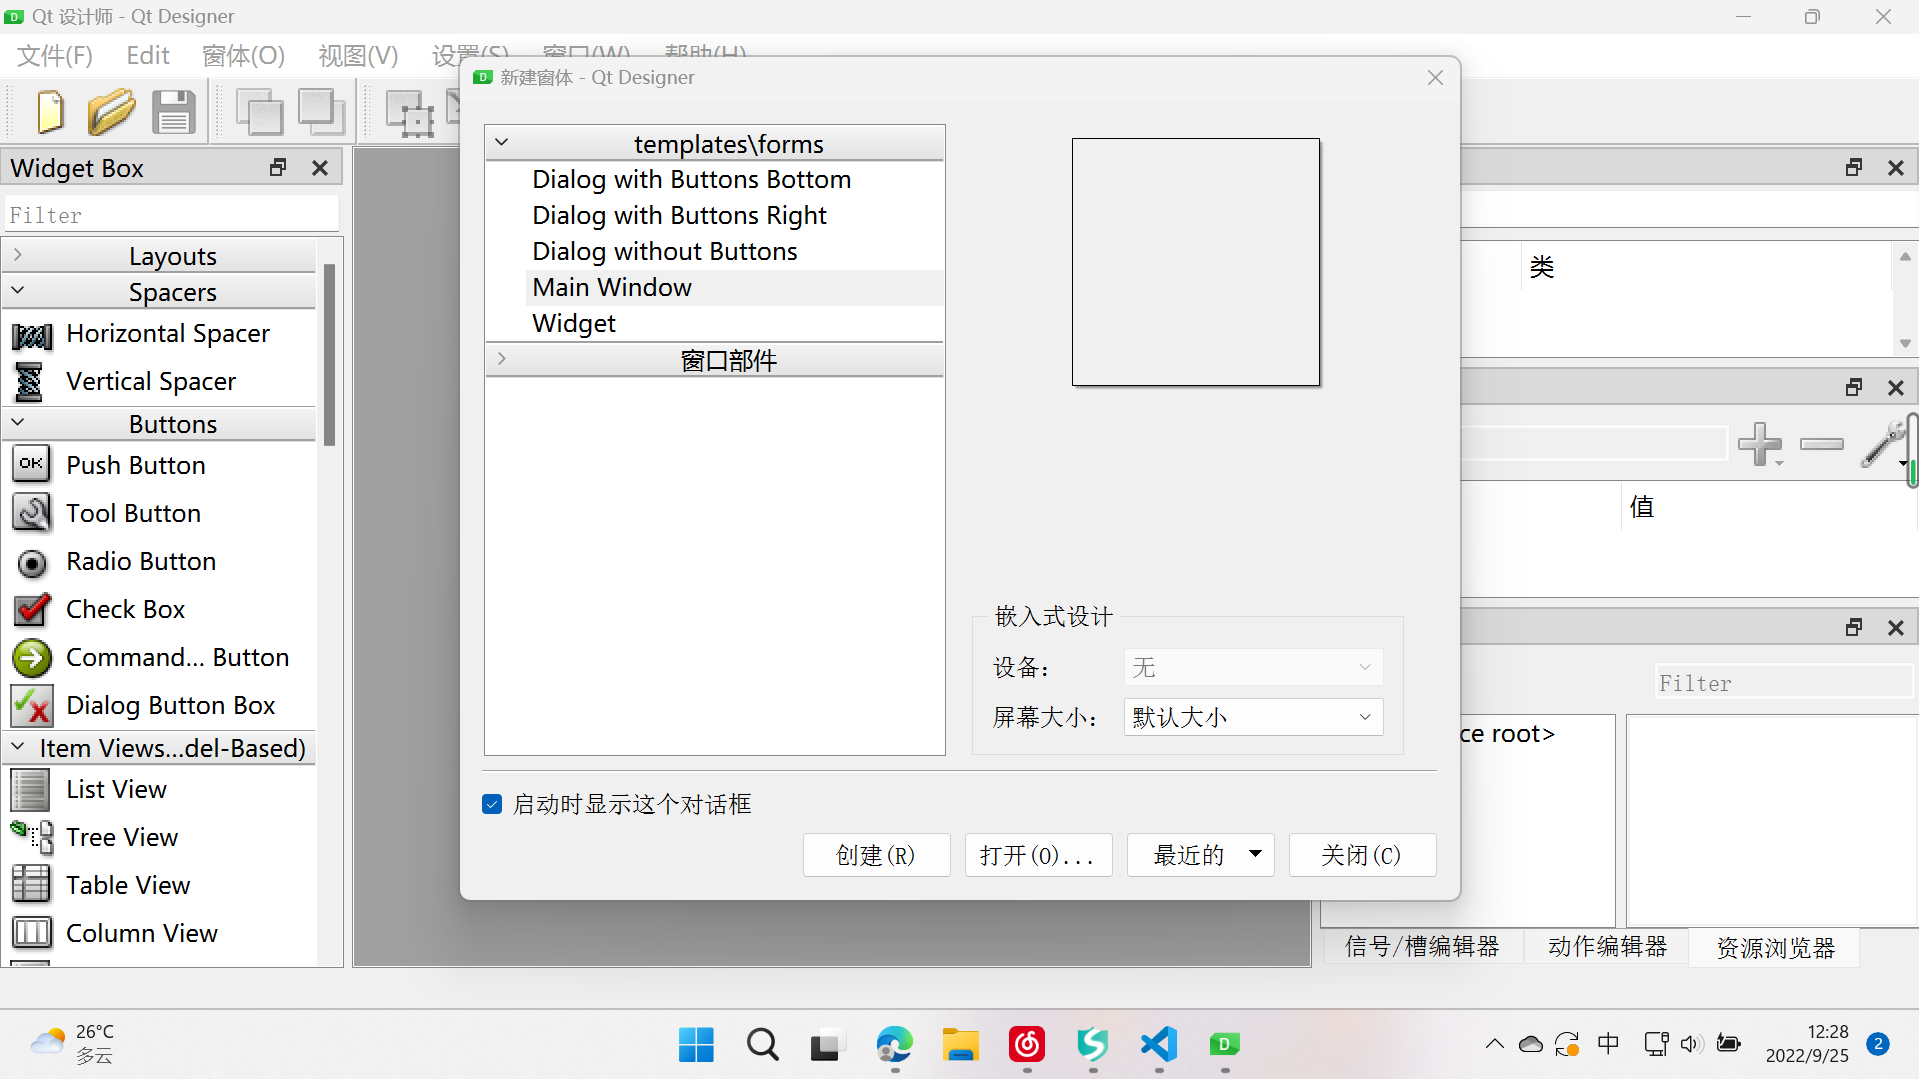
\includegraphics[width=5cm]{1 (9).png}
			\end{minipage}
		}
		\subfigure{
			\begin{minipage}{5cm}
				\centering
				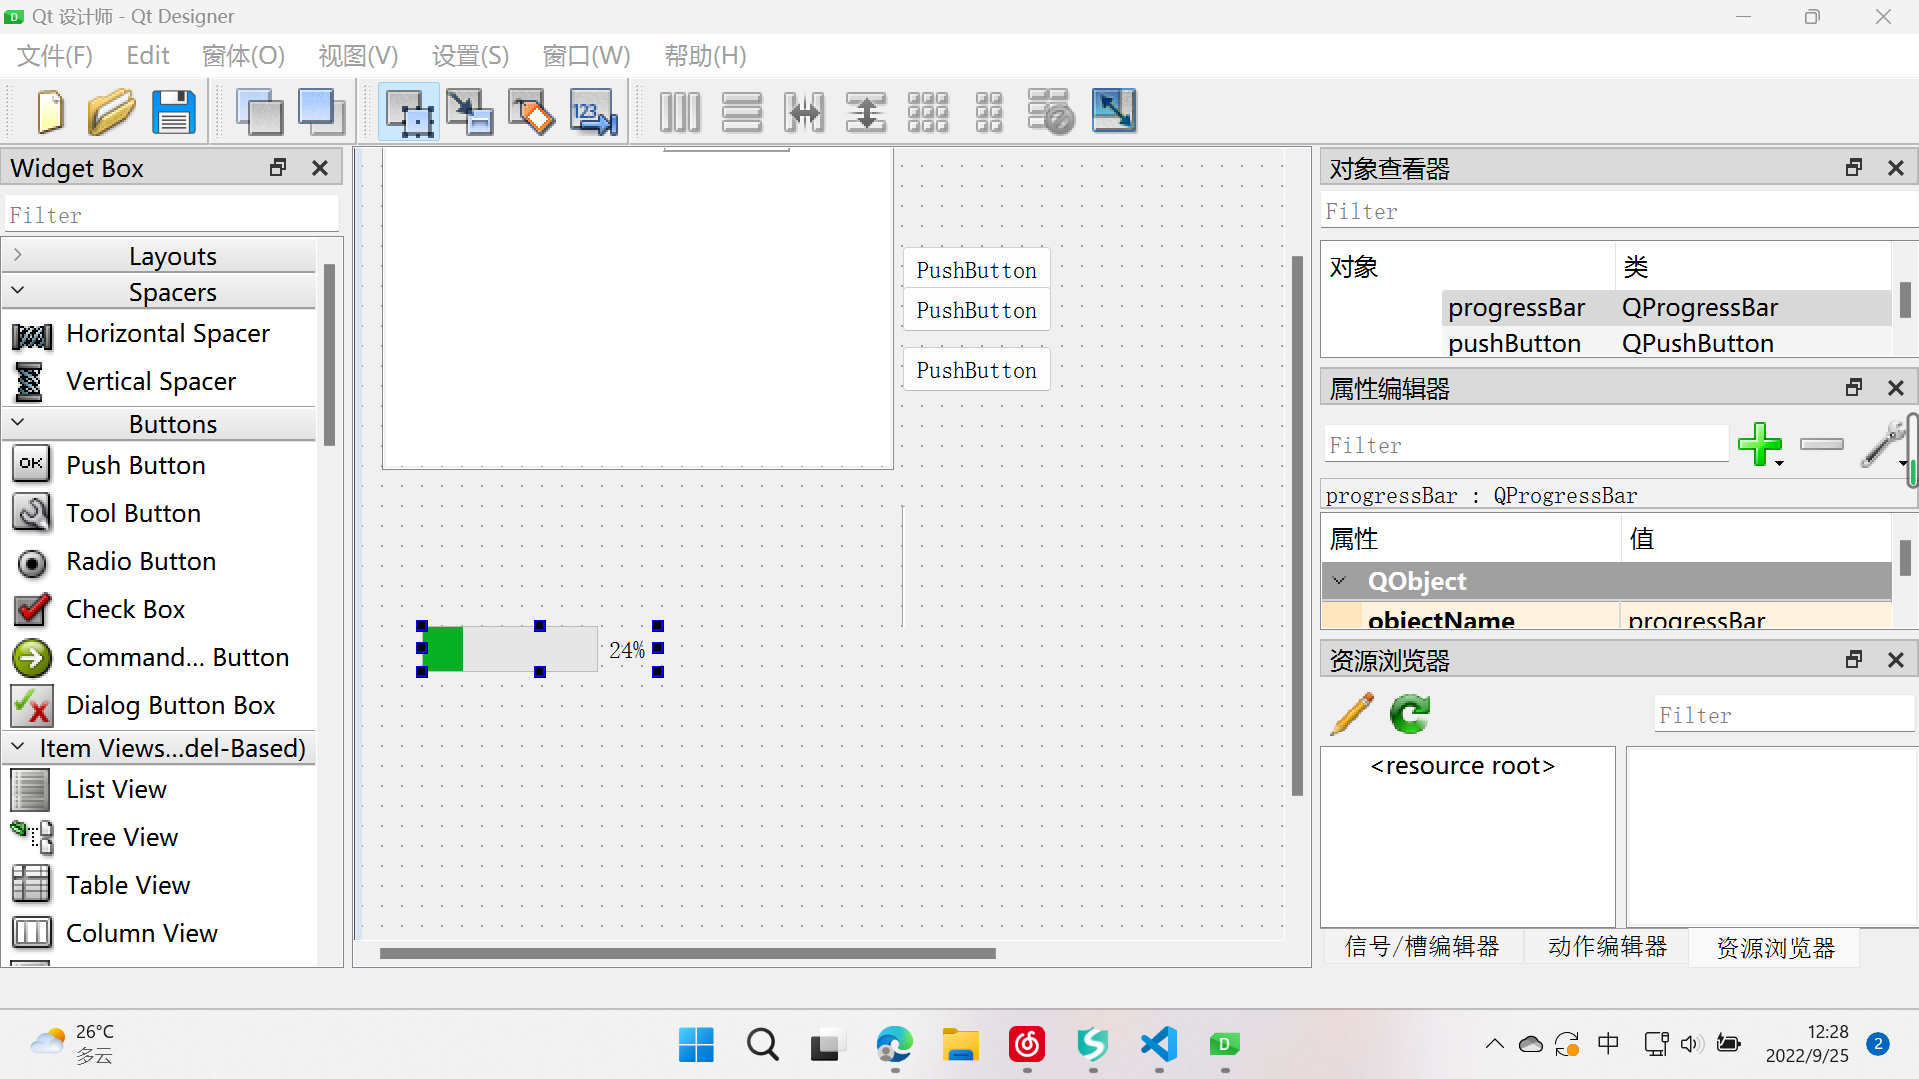
\includegraphics[width=5cm]{1 (10).png}
			\end{minipage}
		}
		\subfigure{
			\begin{minipage}{5cm}
				\centering
				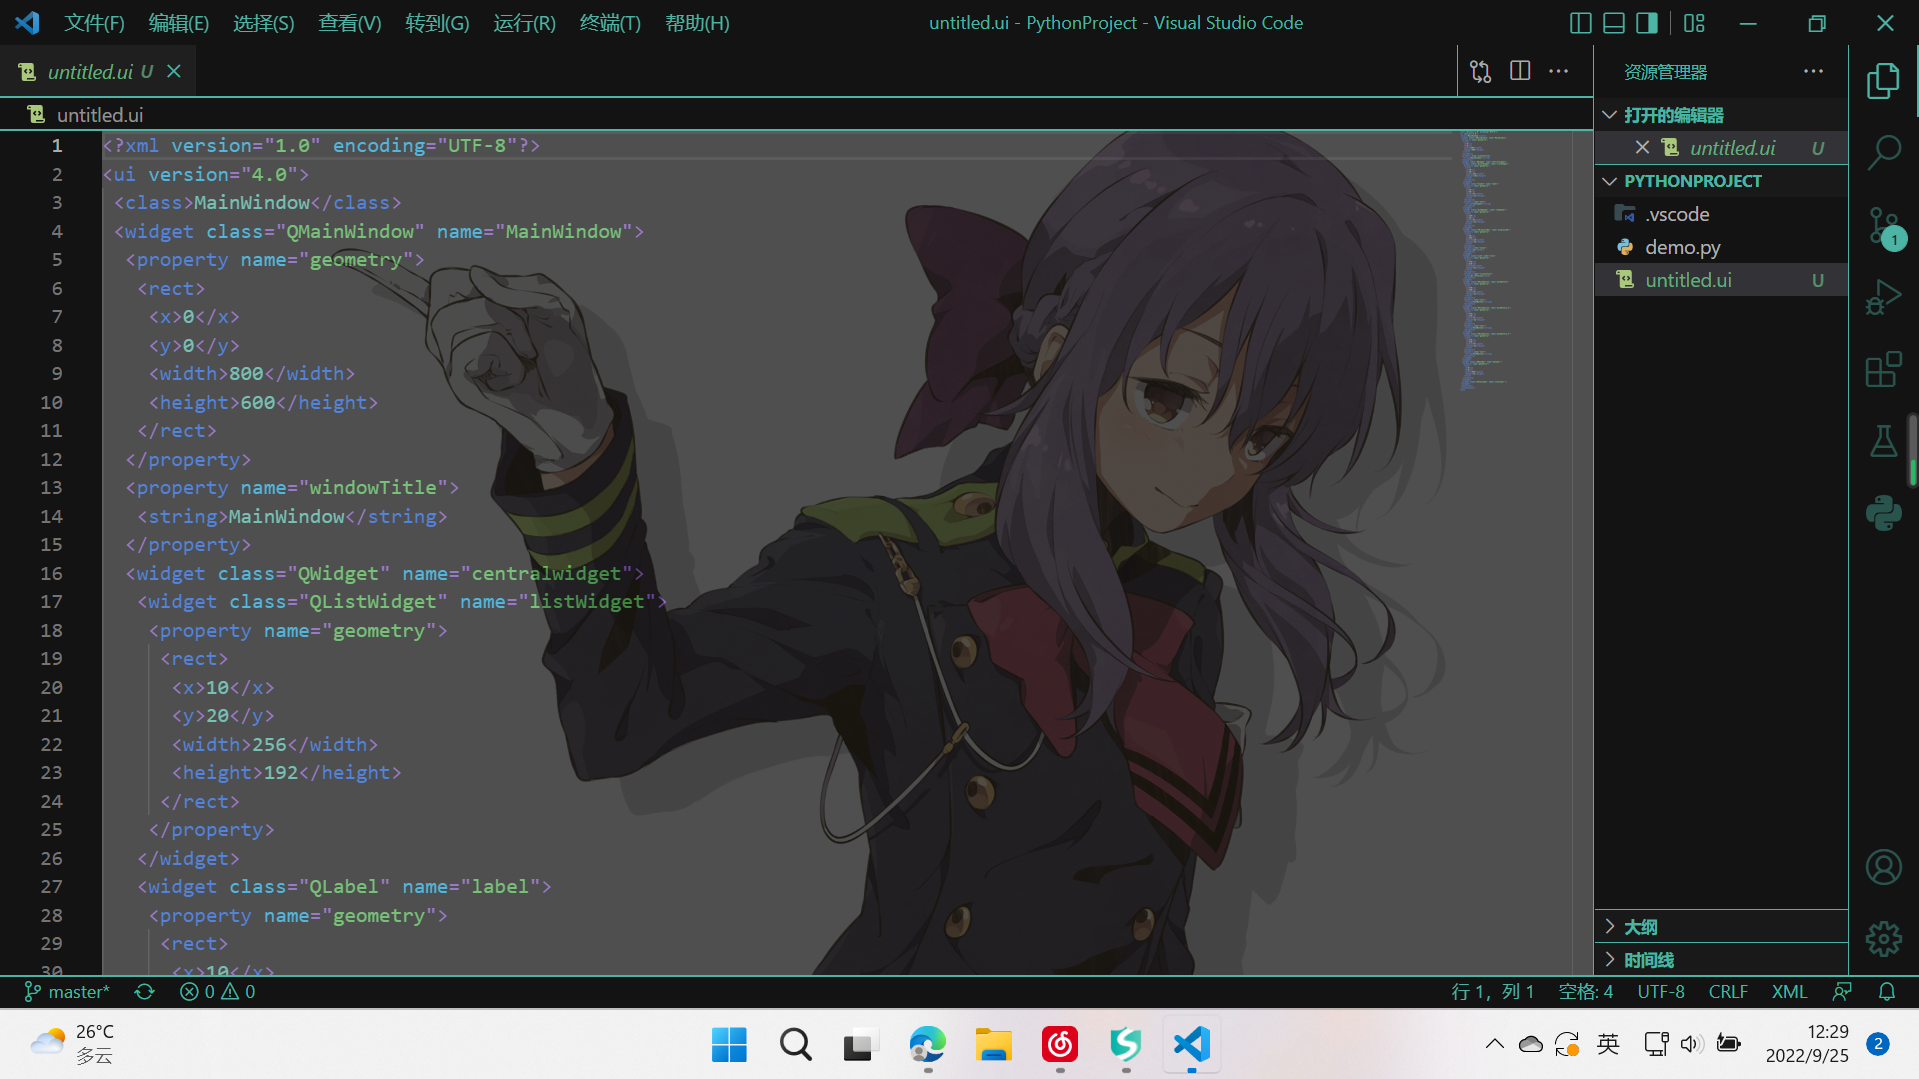
\includegraphics[width=5cm]{1 (11).png}
			\end{minipage}
		}
		\subfigure{
			\begin{minipage}{5cm}
				\centering
				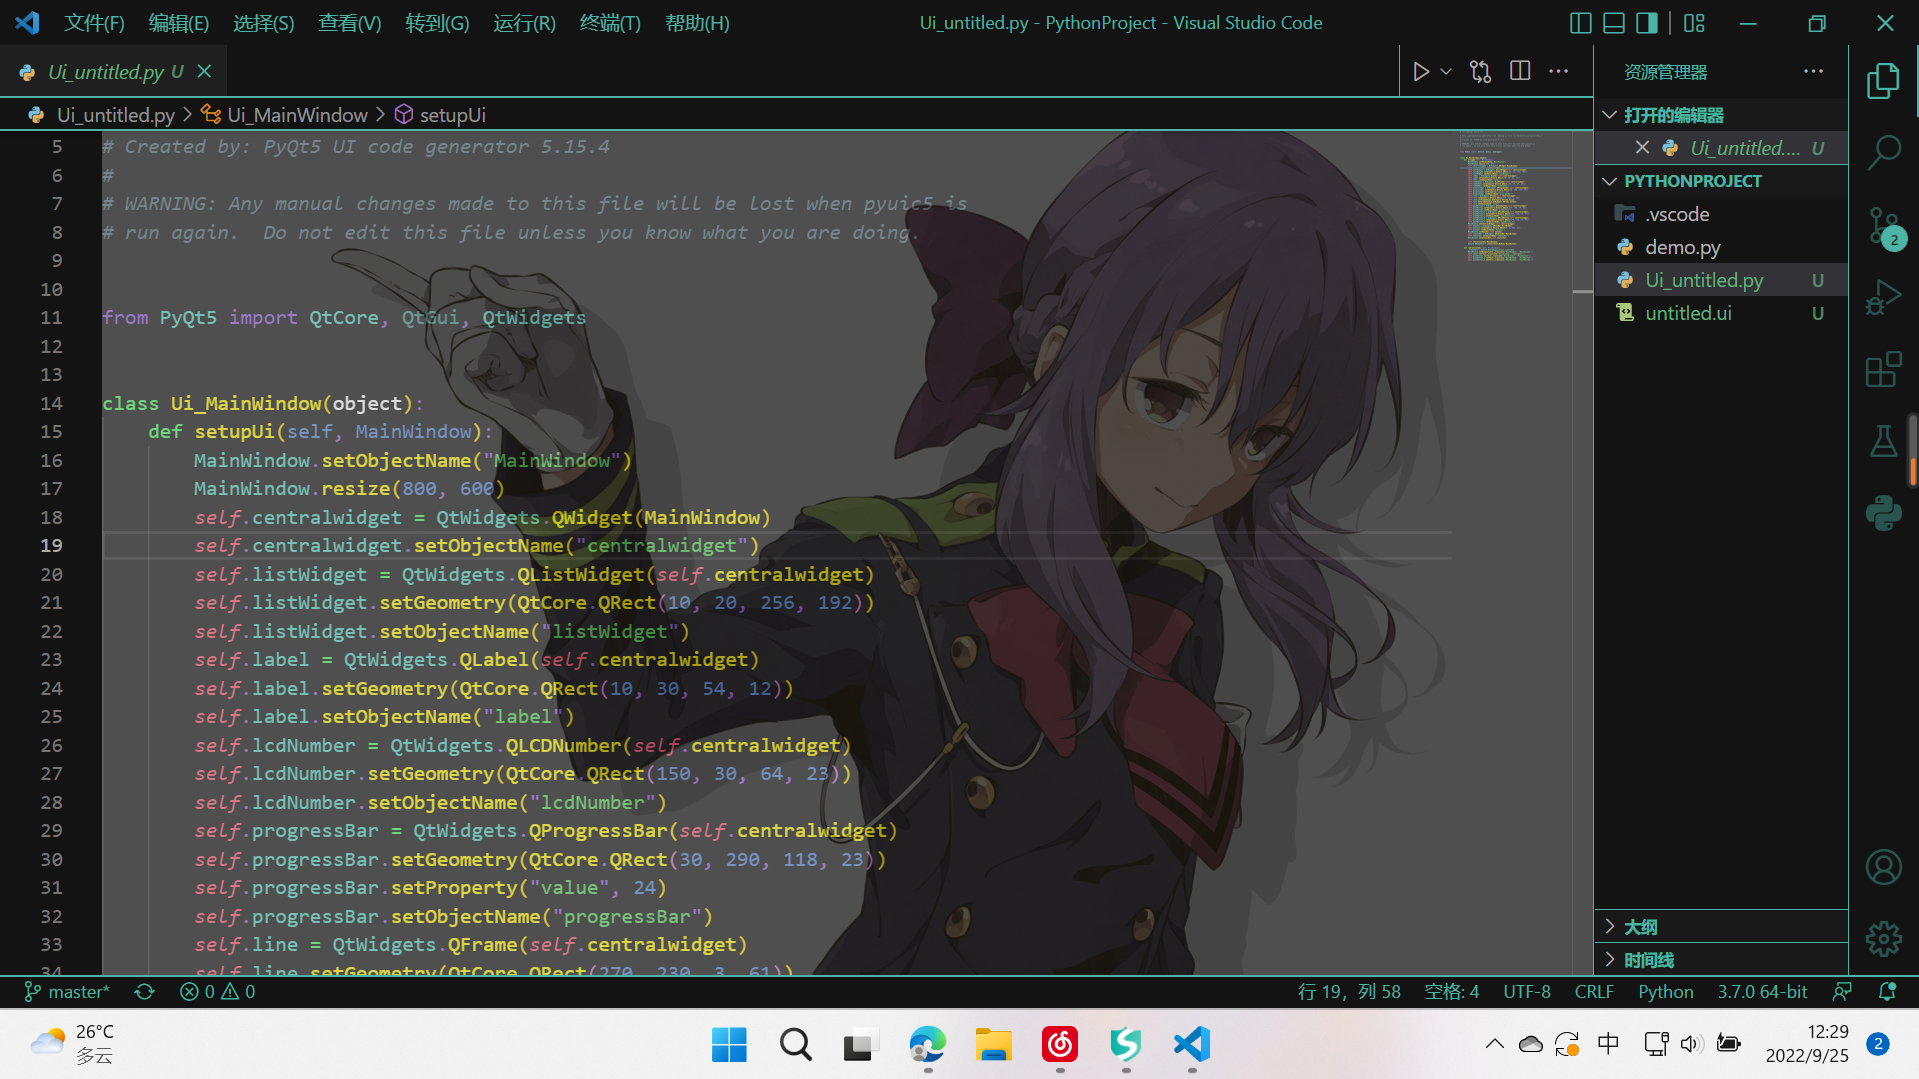
\includegraphics[width=5cm]{1 (12).png}
			\end{minipage}
		}
	\end{figure}
\section{vscode创建本地仓库并上传github}
	初始化仓库后,克隆库,同步后提交,最后发布.
	\begin{figure}[htbp]
		\centering
		\subfigure{
			\begin{minipage}{5cm}
				\centering
				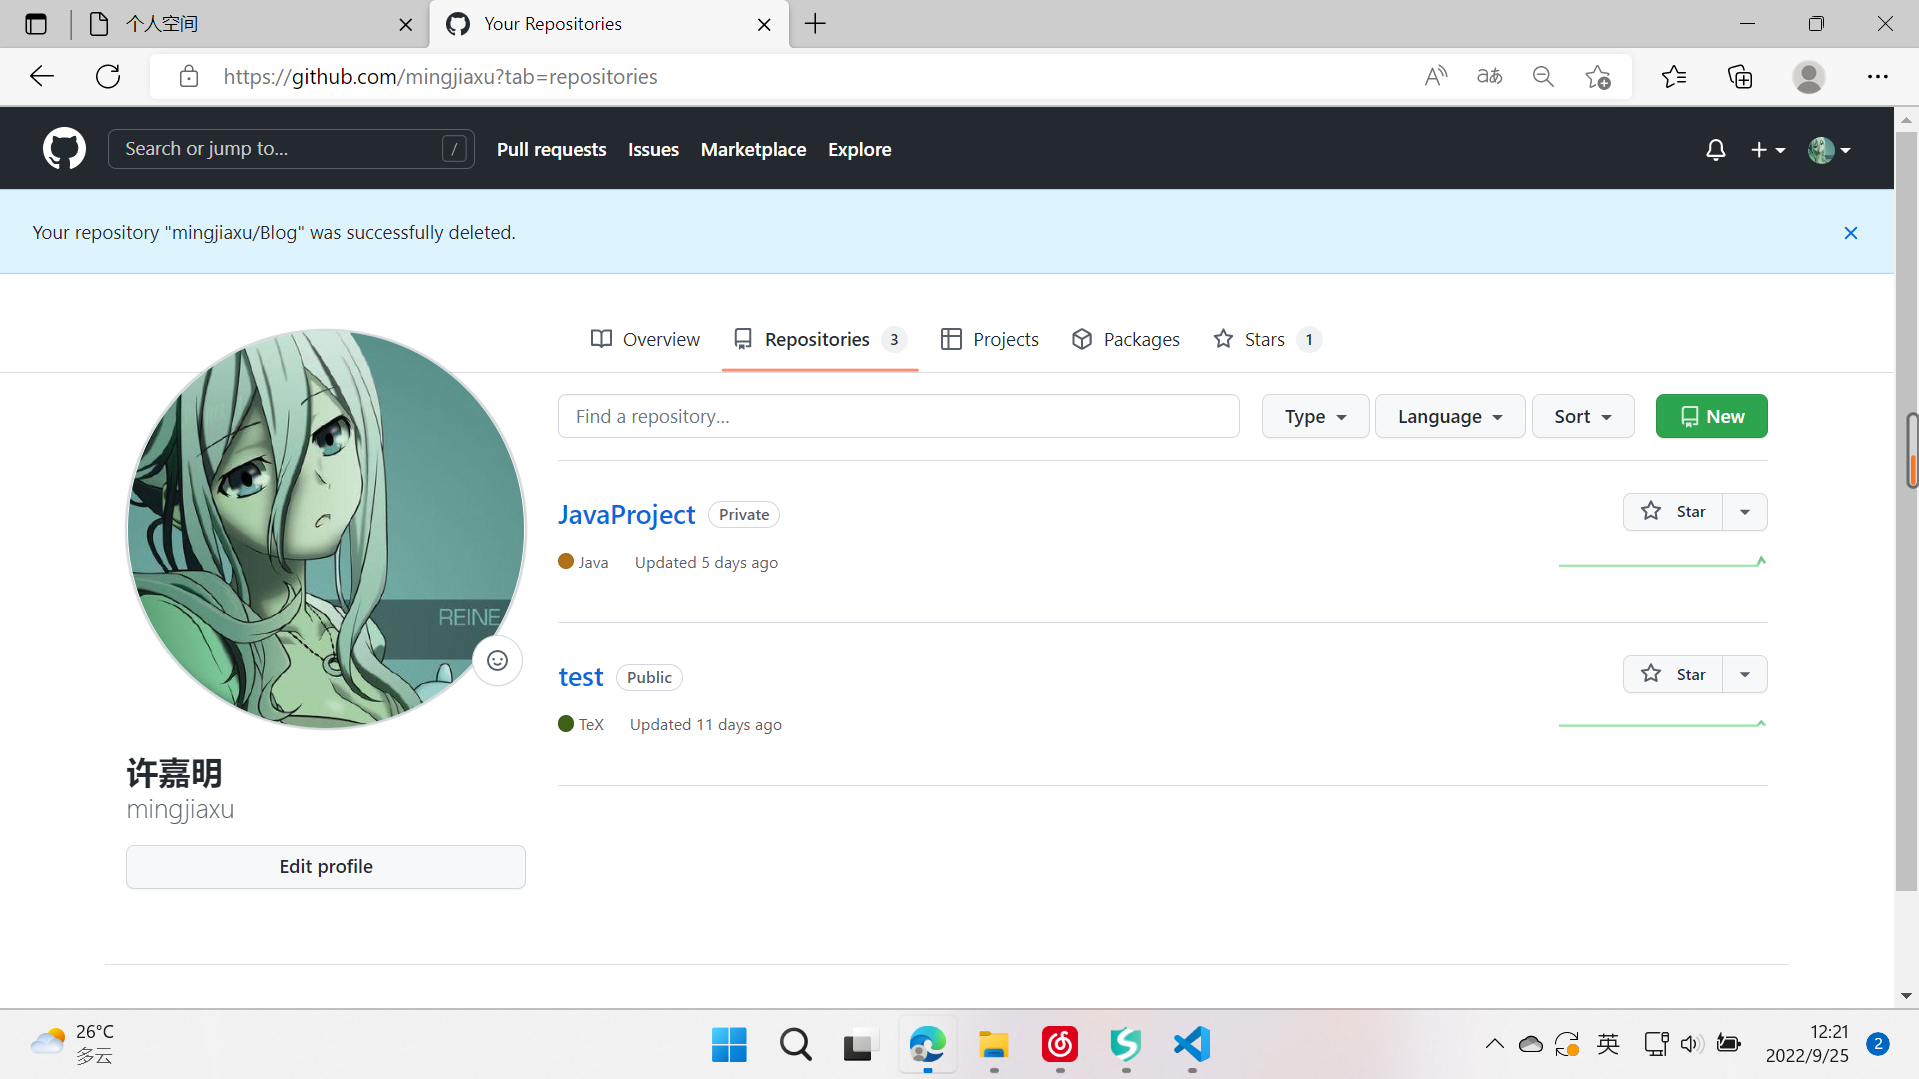
\includegraphics[width=5cm]{1 (1).png}
			\end{minipage}
		}
		\subfigure{
			\begin{minipage}{5cm}
				\centering
				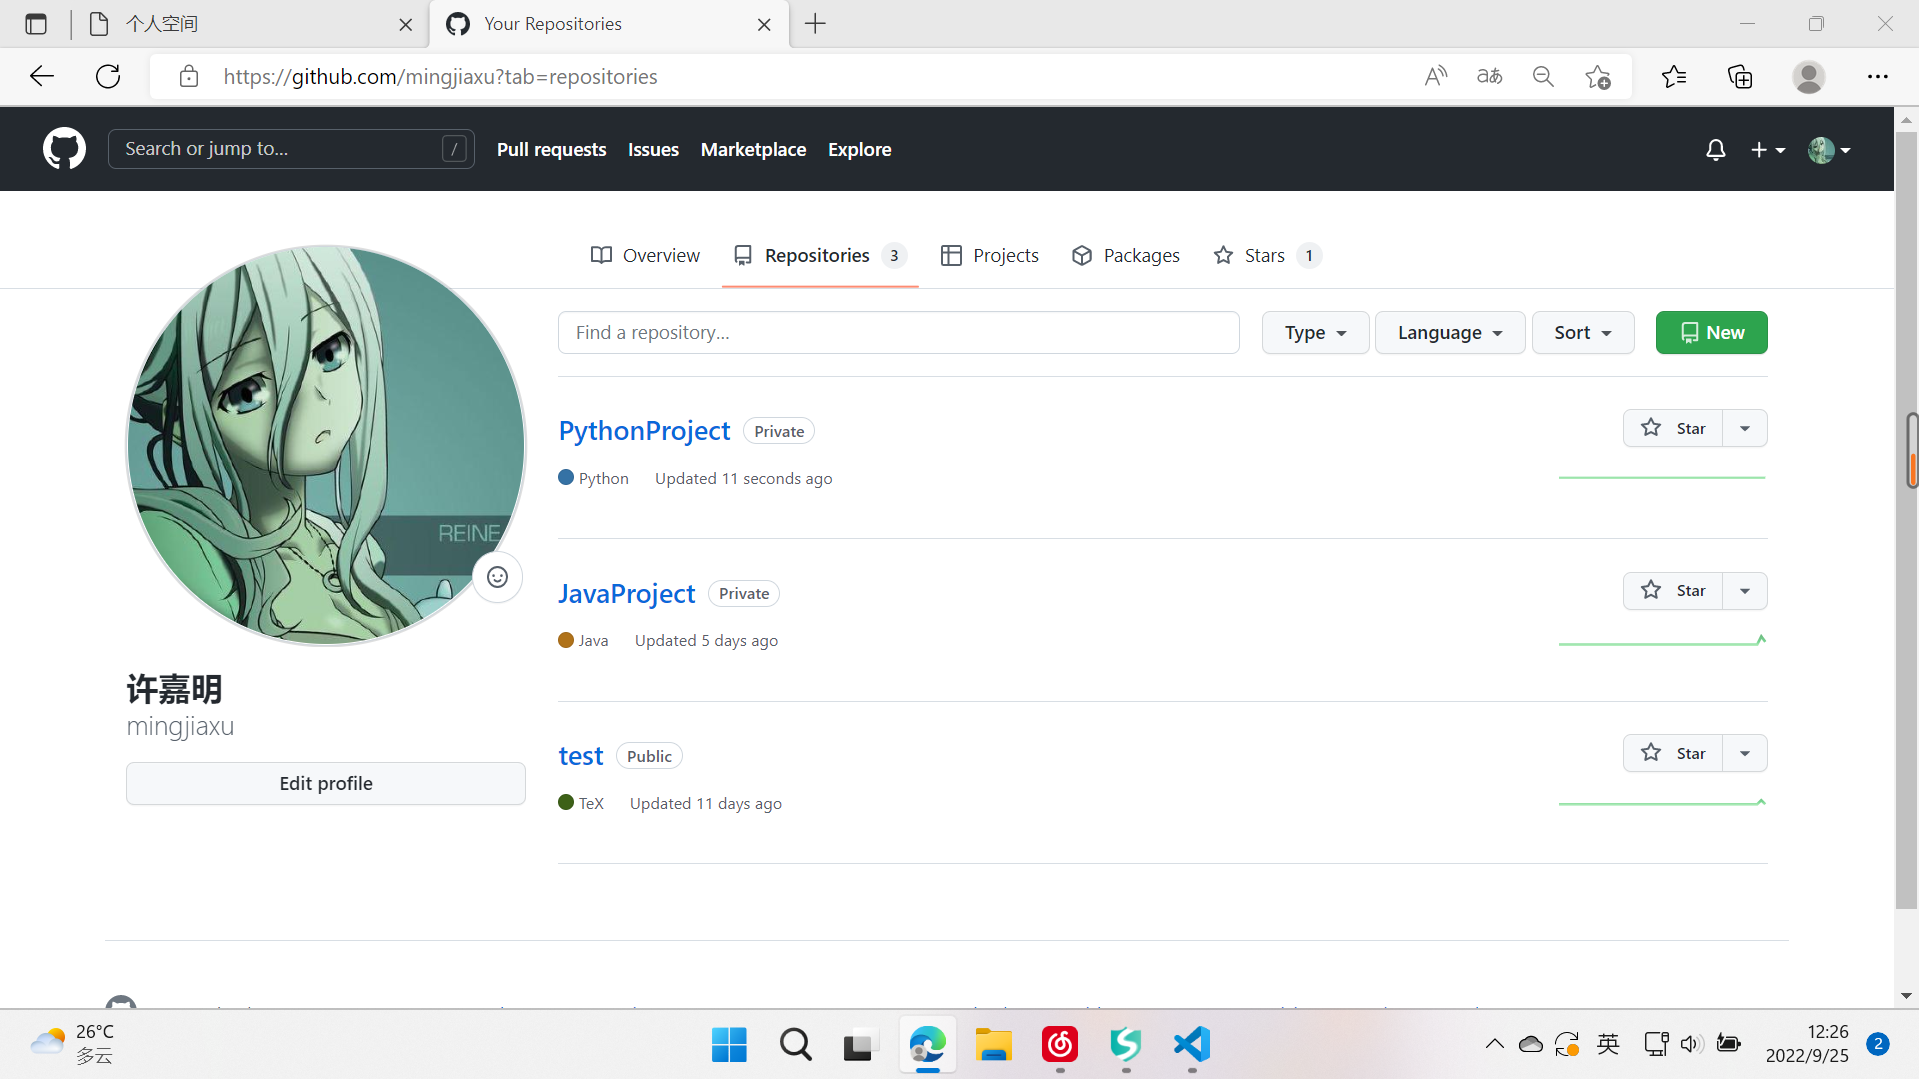
\includegraphics[width=5cm]{1 (7).png}
			\end{minipage}
		}
		\subfigure{
			\begin{minipage}{5cm}
				\centering
				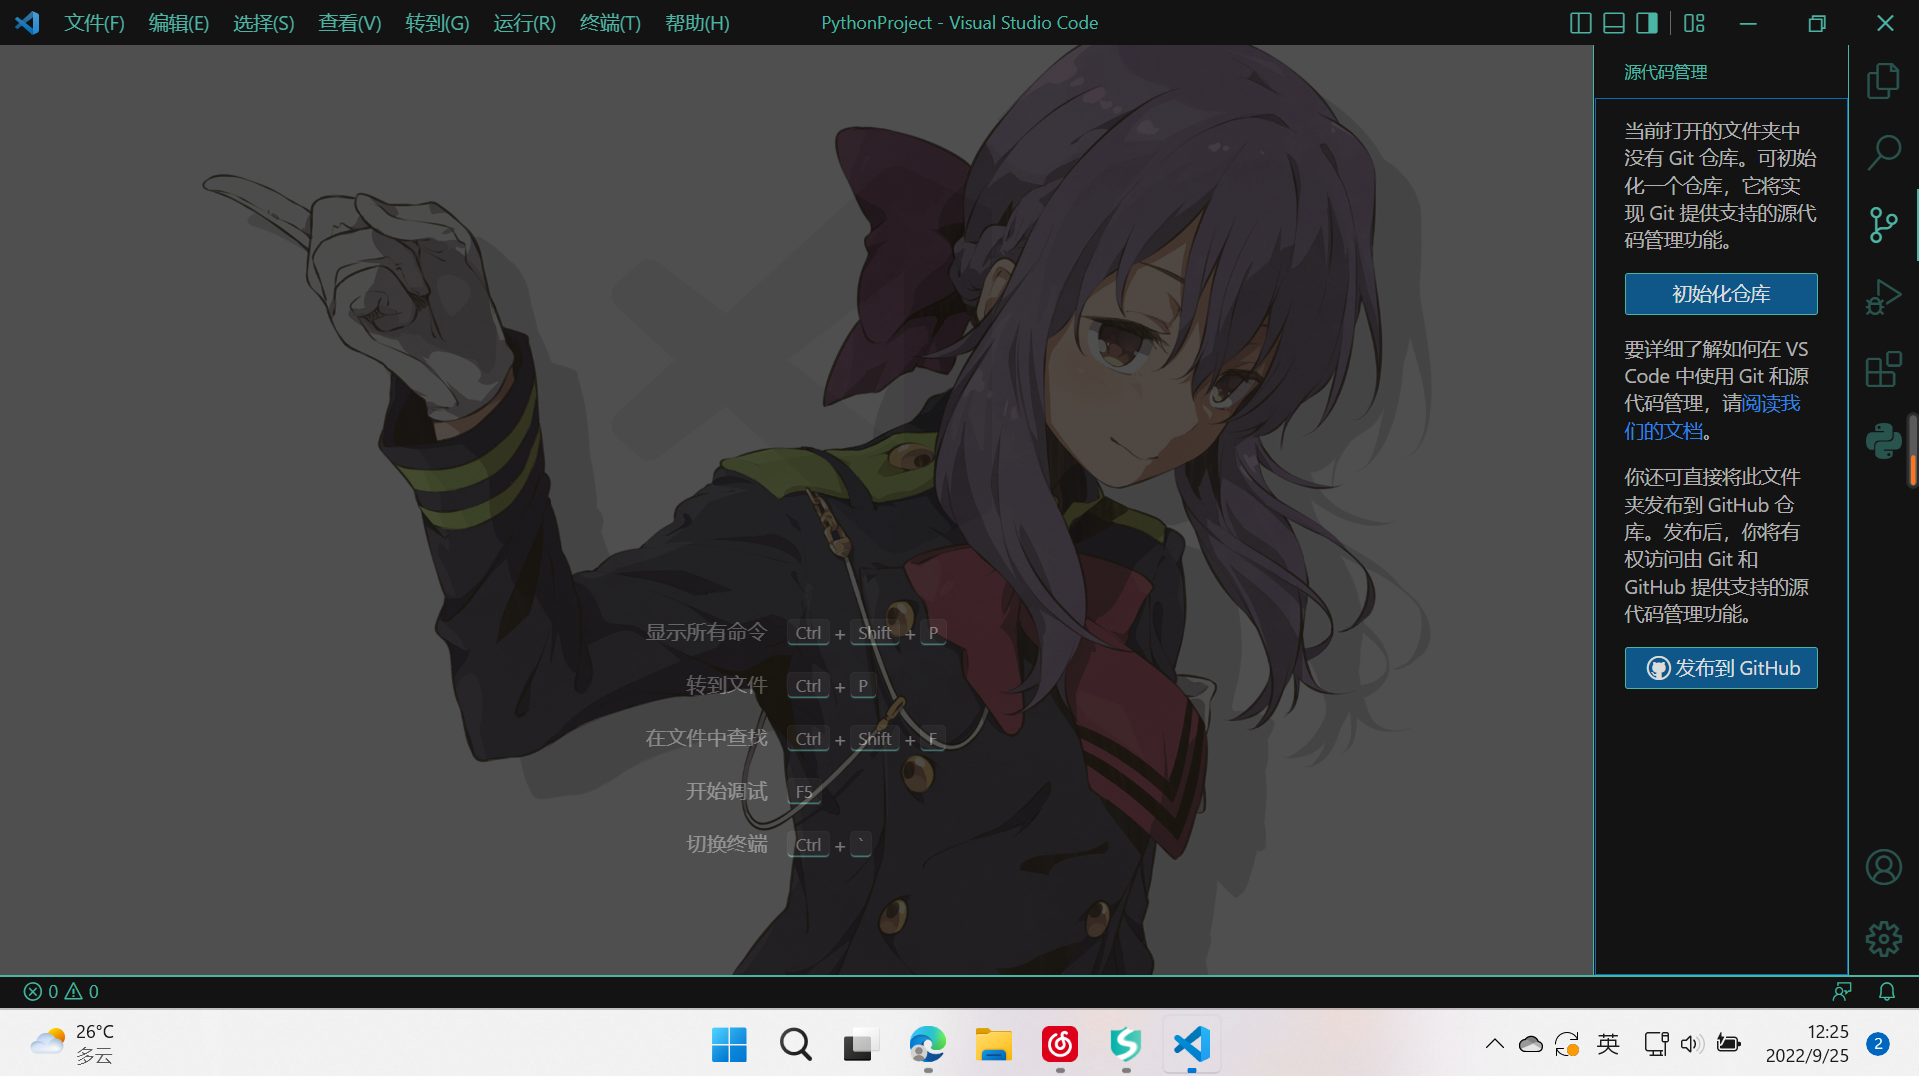
\includegraphics[width=5cm]{1 (3).png}
			\end{minipage}
		}
	\subfigure{
		\begin{minipage}{5cm}
			\centering
			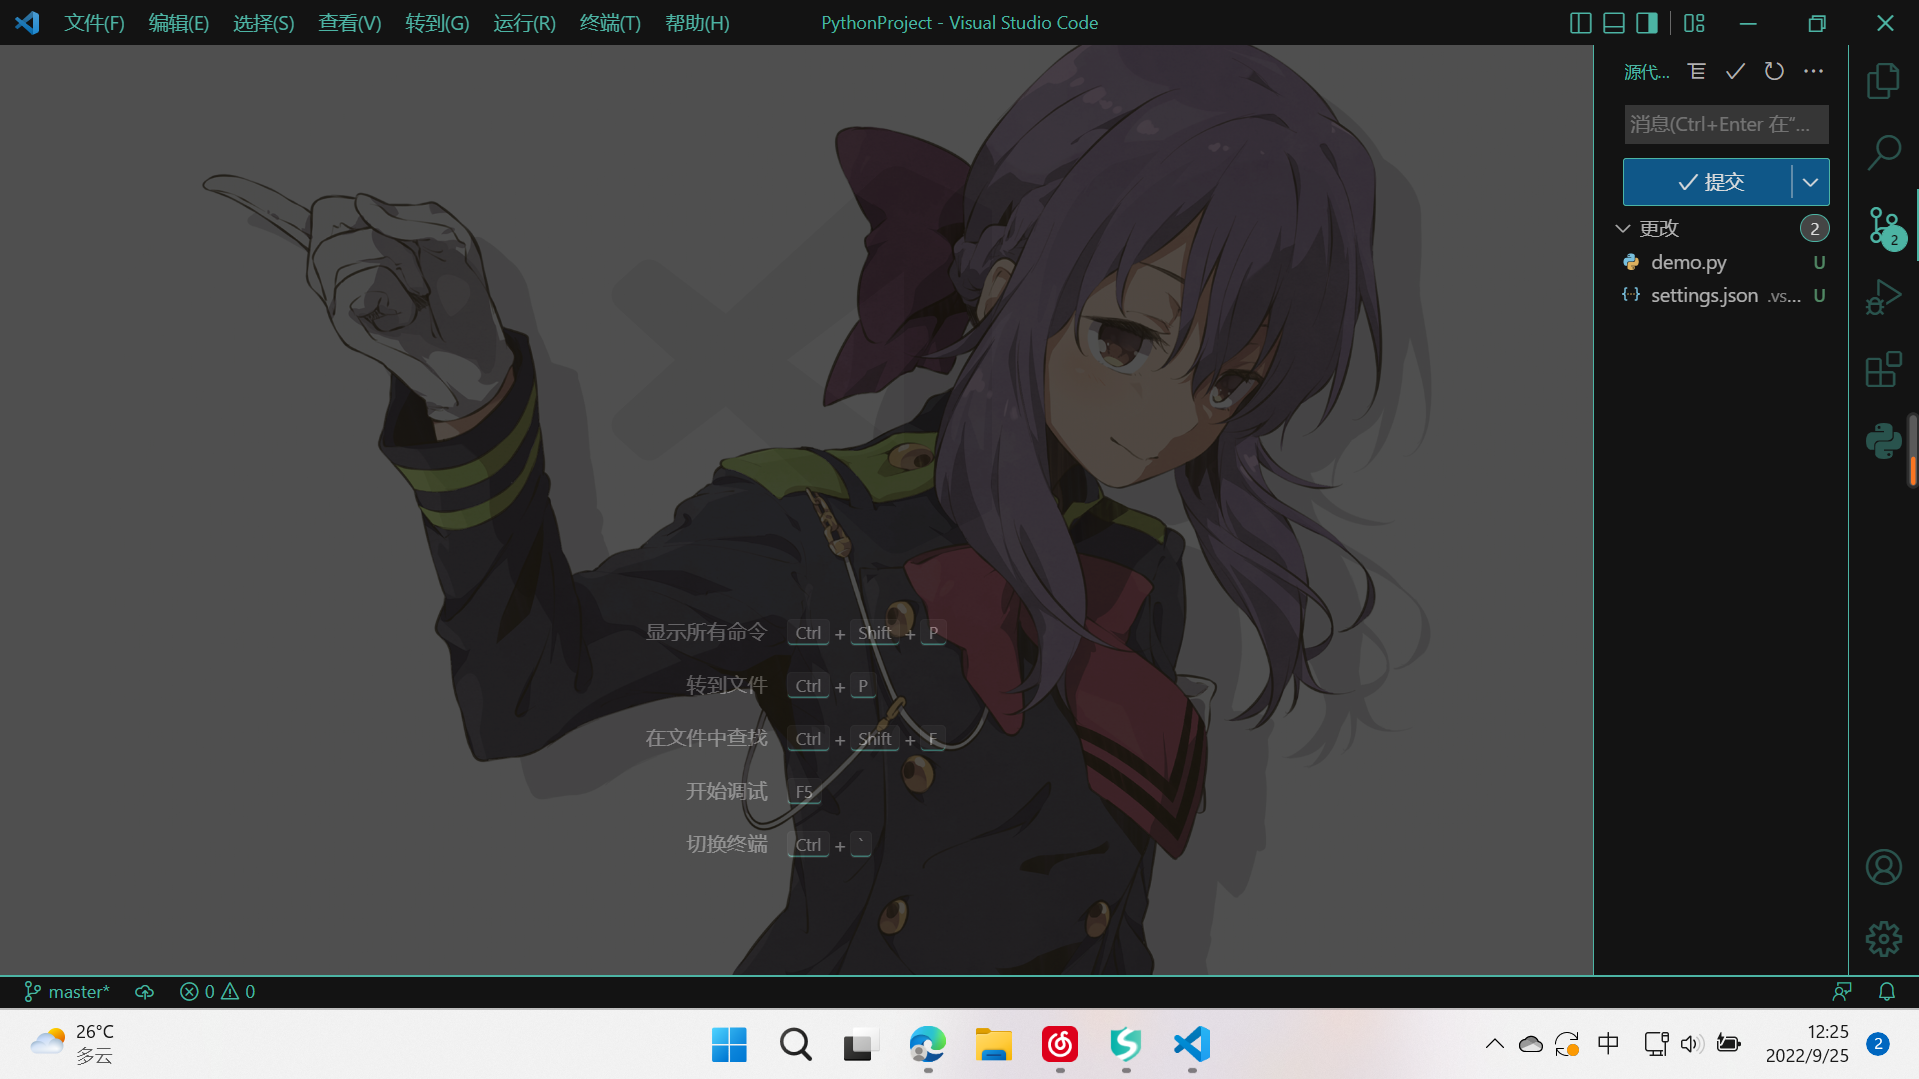
\includegraphics[width=5cm]{1 (4).png}
		\end{minipage}
	}
	\subfigure{
		\begin{minipage}{5cm}
			\centering
			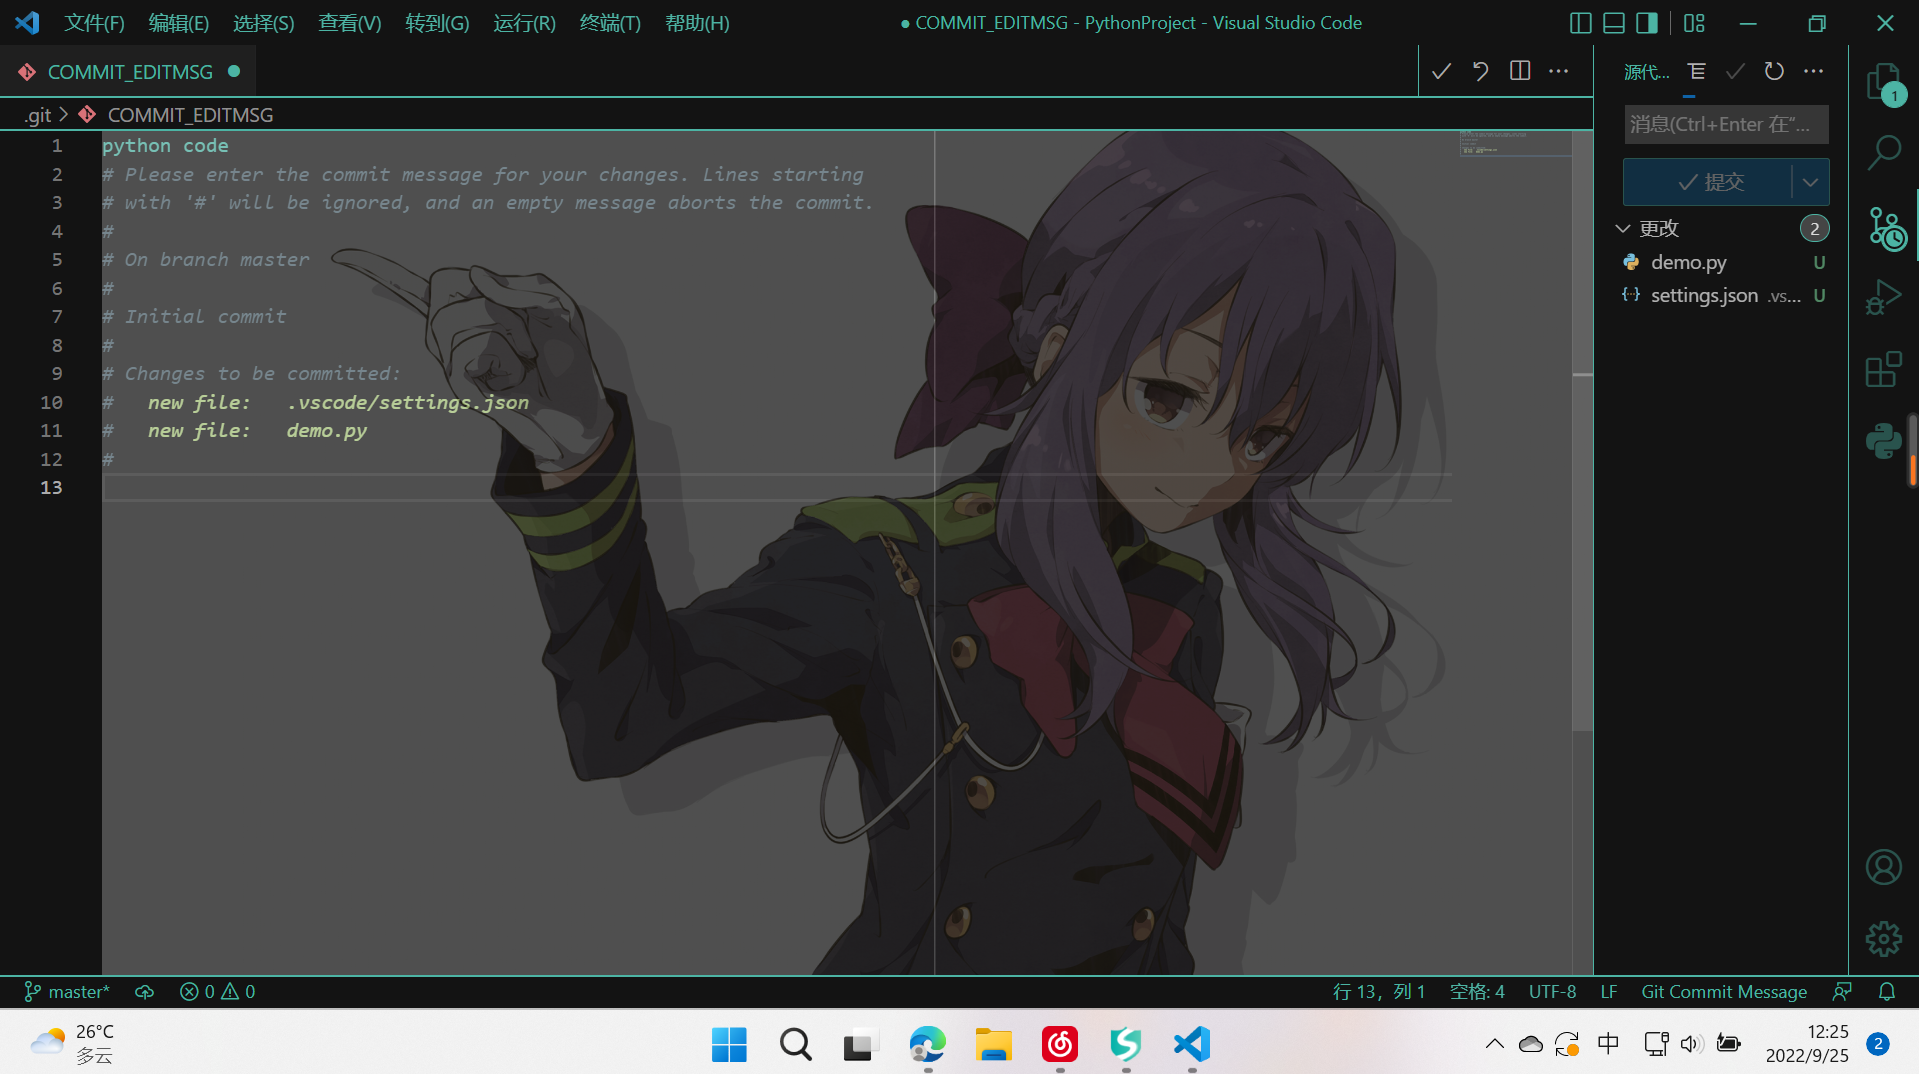
\includegraphics[width=5cm]{1 (5).png}
		\end{minipage}
	}
	\subfigure{
		\begin{minipage}{5cm}
			\centering
			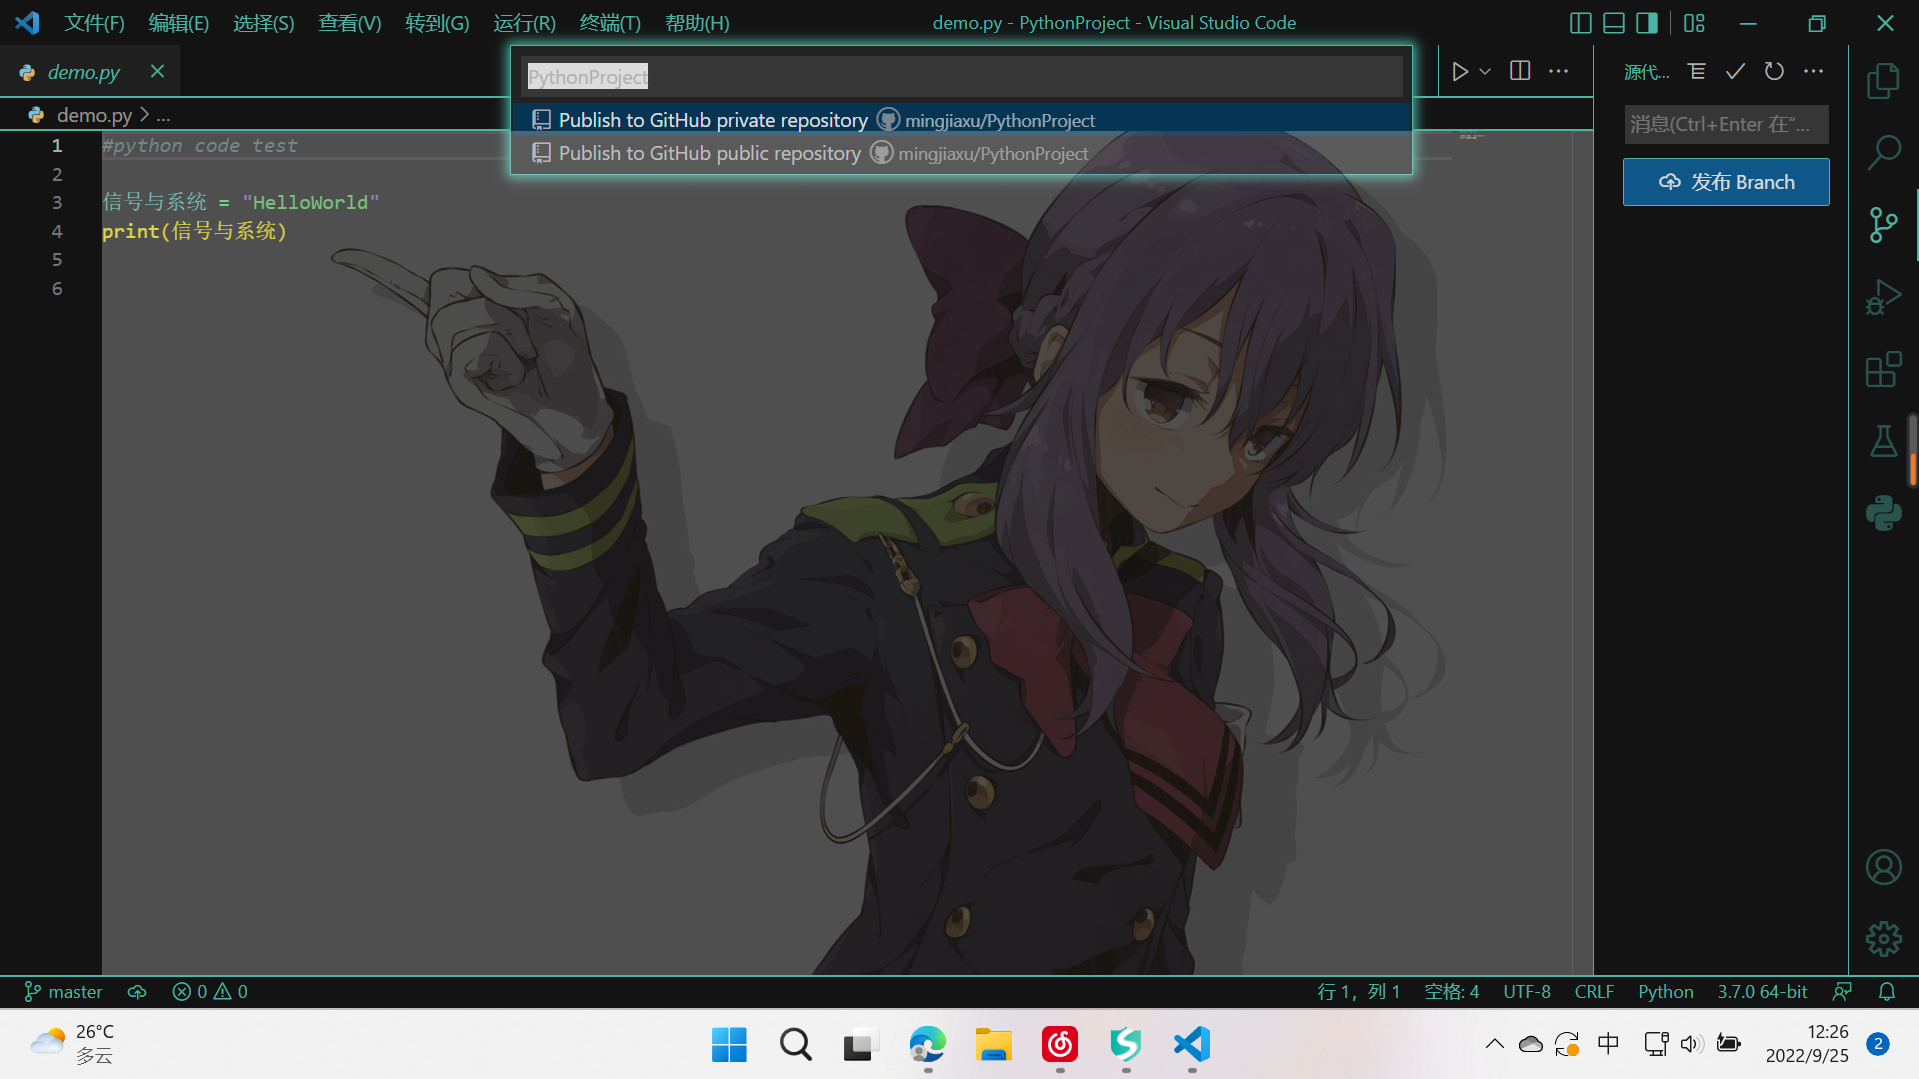
\includegraphics[width=5cm]{1 (6).png}
		\end{minipage}
	}
\end{figure}
\end{document}
